%======================================================================
%  Seccion 6.3 - Prototipo funcional de la Base de Datos
%
%  Para Ferney: este archivo REEMPLAZA toda la subseccion "Prototipo
%  funcional de la Base de Datos" del capitulo 6 (desde su \subsection
%  hasta el final del capitulo). La subseccion 6.3.1 es copia de la
%  existente, con su ultimo parrafo cambiado. Las demas (6.3.2 a 6.3.10)
%  son nuevas. Las cifras y resultados salen de docs/evidence/; junto a
%  cada tabla de resultados un comentario indica el archivo de origen.
%
%  Figuras: las 4 de UML y las 10 capturas estan en la carpeta figures/
%  (junto a este archivo); el texto las incluye como figures/<nombre>.png.
%  Si el proyecto las guarda en otra carpeta, ajuste esas rutas o use
%  \graphicspath. Regenerar: docs/report/figures/generate-figures.sh.
%
%  Usa los paquetes del capitulo 6: longtable, booktabs, array con el tipo
%  de columna L{ancho}, setspace, enumitem, adjustbox, amsmath, listings con
%  el estilo sqlpro (se usa tambien con language=Java), graphicx e
%  hyperref.
%
%  Etiquetas de otros capitulos que usa (deben existir): sec:algebra,
%  sec:almacenamiento, tab:aplicaciones, tab:consultas6, tab:transacciones,
%  tab:informes, tab:reglasnegocio, tab:vistas, tab:transiciones,
%  tab:indices, tab:disparadores, tab:roles, tab:volumen y q:C1 a q:C10.
%
%  Orden: 6.3.1 arquitectura, 6.3.2 base de datos, 6.3.3 datos de prueba,
%  6.3.4 consultas, 6.3.5 transacciones, 6.3.6 informes, 6.3.7 aplicacion,
%  6.3.8 extensiones, 6.3.9 concurrencia, 6.3.10 despliegue.
%======================================================================

\subsection{Prototipo funcional de la Base de Datos}
\label{sec:prototipo}

\subsubsection{Arquitectura del prototipo}
\label{sec:arquitectura}

El prototipo se organiza como una arquitectura en cuatro capas lógicas.
Cada capa tiene una sola responsabilidad y solo usa la capa que está
debajo de ella:

\begin{enumerate}[itemsep=2pt]
  \item \textbf{Presentación.} Las aplicaciones de la
        tabla~\ref{tab:aplicaciones}: muestran formularios, planillas e
        informes, capturan los datos y validan solo su formato. No
        deciden reglas del negocio.
  \item \textbf{Casos de uso.} Un servicio por cada grupo de casos de
        uso del módulo (recolección, centro, ruta, servicio al cliente,
        indicadores y administración). Cada operación verifica el rol
        del usuario, abre la transacción, pide al dominio que aplique las
        reglas, manda guardar y confirma o deshace todo
        (tabla~\ref{tab:transacciones}).
  \item \textbf{Modelo de dominio.} Las entidades del modelo conceptual
        convertidas en clases con comportamiento, agrupadas alrededor
        del envío (con sus eventos, destinatario, prueba y novedades) y
        del despacho (con sus asignaciones). Aquí se aplican las reglas
        de negocio de la tabla~\ref{tab:reglasnegocio}, como las
        transiciones de estado (tabla~\ref{tab:transiciones}) o el
        máximo de intentos, antes de tocar la base de datos.
  \item \textbf{Datos.} Los repositorios que leen y guardan las entidades
        mediante JDBC, con las consultas de la sección~\ref{sec:algebra}
        y las vistas de usuario, y la base de datos Oracle con las
        restricciones, disparadores, índices y roles del capítulo 5.
\end{enumerate}

La presentación se ejecuta en los equipos de los usuarios; las capas de
casos de uso, dominio y acceso a datos, en el servidor de aplicaciones;
y la base de datos, en su propio servidor (sección~\ref{sec:almacenamiento}).
Las reglas de negocio se verifican dos veces: en el dominio, para
explicar al usuario qué falló antes de intentar guardar, y en la base de
datos, como garantía final aunque alguien llegue a ella por otro camino.

\textbf{Por qué no Oracle REST Data Services.} Oracle ofrece una
herramienta, Oracle REST Data Services (ORDS), que publica directamente
las tablas, vistas y procedimientos de la base de datos como servicios
web, sin escribir un servidor de aplicaciones. Se descartó como base del
prototipo porque las aplicaciones hablarían directamente con la base de
datos y se saltarían las capas de casos de uso y de dominio, lo que trae
estos problemas:

\begin{itemize}[itemsep=2pt]
  \item \textbf{Transacciones incompletas.} Operaciones como registrar
        una entrega insertan la prueba, actualizan la asignación e
        insertan el evento. Sin una capa que las agrupe, la aplicación
        tendría que hacer varias llamadas independientes; si la conexión
        del mensajero se cae en medio, la operación queda a medias.
  \item \textbf{Reglas repartidas.} Para dar mensajes claros, cada
        aplicación (web, móvil y portal) tendría que repetir las reglas
        de negocio por su cuenta, con el riesgo de que difieran entre sí
        y de la base de datos.
  \item \textbf{Aplicaciones atadas a las tablas.} Los servicios
        reflejarían la estructura de las tablas, así que cualquier cambio
        del esquema, como las columnas que se agregarán al integrar el
        módulo de facturación, obligaría a cambiar todas las
        aplicaciones.
  \item \textbf{Control de acceso más pobre.} Los permisos quedarían a
        nivel de tabla y no de caso de uso: es difícil expresar, por
        ejemplo, que un mensajero solo puede registrar resultados en sus
        propios despachos, y quedaría expuesta a internet una superficie
        mayor de la base de datos.
\end{itemize}

ORDS podría usarse más adelante para publicar consultas de solo lectura,
como el seguimiento del portal, sin afectar esta arquitectura.

Las subsecciones siguientes construyen el prototipo con esta
arquitectura. La subsección~\ref{sec:proto-bd} crea la base de datos del
módulo en el gestor, con los objetos físicos del capítulo~5, y comprueba
que coincide con el diseño; la~\ref{sec:proto-datos} carga los datos de
prueba. Después se ejecutan las consultas de la
sección~\ref{sec:algebra} (subsección~\ref{sec:proto-consultas}), las
transacciones de la tabla~\ref{tab:transacciones} con sus reglas de
negocio (\ref{sec:proto-transacciones}) y los informes de la
tabla~\ref{tab:informes} (\ref{sec:proto-informes}), y se muestran sus
resultados. Por último se presentan la aplicación que demuestra el flujo
principal (\ref{sec:proto-aplicacion}), las extensiones fuera del módulo
(\ref{sec:proto-extensiones}), el comportamiento con accesos
simultáneos (\ref{sec:proto-concurrencia}) y el despliegue
(\ref{sec:proto-despliegue}).

%-----------------------------------------------------------------------
\subsubsection{Implementación de la base de datos y verificación de cifras}
\label{sec:proto-bd}

\textbf{Entorno.} La base de datos es Oracle Database 23c, edición Free,
que corre en un contenedor Docker definido con docker compose. La base
conectable de trabajo es FREEPDB1 y el contenedor y la aplicación usan
la zona horaria America/Bogota. La versión instalada se identifica como
Oracle AI Database 26ai Free (versión 23.26.4): es la misma línea 23 que
Oracle renombró primero 23ai y después 26ai, de modo que coincide con la
del capítulo~5. El juego de caracteres es AL32UTF8 y las longitudes de
texto se cuentan en caracteres, como se definió en ese capítulo.

\textbf{Scripts.} La base se construye con scripts SQL y PL/SQL
numerados en la carpeta \texttt{database/}; la tabla~\ref{tab:proto-scripts}
resume qué contiene cada carpeta y con qué cuenta se ejecuta. Un solo
comando, \texttt{database/install.sh}, reinstala todo desde cero: limpia el
esquema, ejecuta las carpetas en orden y termina con la verificación de
cifras de esta subsección. Con los datos fijos tarda unos 5 segundos y
con los datos de volumen, unos 49. El comando
\texttt{database/generate-evidence.sh} repite en cadena la instalación, las
pruebas, las consultas, las transacciones, los informes y los planes de
ejecución, y guarda sus resultados en \texttt{docs/evidence/}; la
corrida completa (17 pasos, todos OK) tardó 81 segundos
(\texttt{docs/evidence/00\_generar\_evidencias.txt}).

{\singlespacing\small
\begin{longtable}{L{3.3cm} L{2.4cm} L{8.7cm}}
\caption{Carpetas de scripts de la base de datos.}
\label{tab:proto-scripts}\\
\toprule
\textbf{Carpeta} & \textbf{Cuenta} & \textbf{Contenido} \\
\midrule
\endfirsthead
\toprule
\textbf{Carpeta} & \textbf{Cuenta} & \textbf{Contenido} \\
\midrule
\endhead
\bottomrule
\endfoot
\texttt{admin} & SYSTEM & Limpieza, los 2 espacios de tablas, el esquema propietario BD\_ENLACE\_EXPRESS, los 5 roles, las 5 cuentas de servicio y los privilegios que usan las extensiones. \\
\texttt{schema} & Propietario & Las 19 tablas, los 59 índices y las 7 vistas. \\
\texttt{plsql} & Propietario & Los paquetes de errores y de calendario, el procedimiento de registro del envío y los 6 disparadores. \\
\texttt{grants} & Propietario & Privilegios de cada rol sobre tablas y vistas, sin DELETE (RN16). \\
\texttt{seed} & Propietario & Catálogos, datos de referencia, operación de noviembre de 2026 y ajuste de las columnas de identidad; en la carpeta \texttt{volumen}, el conjunto de volumen. \\
\texttt{queries} & Cuenta de servicio de cada usuario & Las consultas C1 a C10 y el comando que las ejecuta. \\
\texttt{transactions} & Cuenta de servicio de cada usuario & Las 12 transacciones y la prueba de concurrencia. \\
\texttt{reports} & Cuenta de servicio de cada usuario & Los 7 informes y los planes de ejecución (\texttt{explain}). \\
\texttt{extensions} & Propietario & Extensiones fuera del módulo (subsección~\ref{sec:proto-extensiones}). \\
\texttt{tests} & SYSTEM y propietario & Verificación de cifras y pruebas de reglas, de permisos y de las extensiones. \\
\end{longtable}
\par}

\textbf{Qué se completó respecto al modelo.} El DDL se exportó de
Oracle SQL Developer Data Modeler, donde se construyó el modelo del
capítulo~4. Esa exportación trae las tablas, las columnas, las
restricciones NOT NULL, DEFAULT, PRIMARY KEY, UNIQUE, FOREIGN KEY y CHECK
y los comentarios, y coincide con el documento. Los scripts de
\texttt{database/} le agregan lo que el capítulo~5 define y el modelo lógico no
tiene:

\begin{itemize}[itemsep=2pt]
  \item la semántica de caracteres (longitudes en caracteres) y las
        14 columnas de identidad de las tablas con clave generada;
  \item los espacios de tablas: las tablas en TS\_ENLACE\_DATOS y los
        índices, incluidos los de las claves primarias y únicas, en
        TS\_ENLACE\_INDICES;
  \item los 27 índices adicionales de la tabla~\ref{tab:indices}: 22
        sobre claves foráneas y 5 sobre columnas de consulta frecuente;
  \item las 7 vistas de la tabla~\ref{tab:vistas};
  \item el paquete \texttt{pkg\_errores}, el procedimiento de registro del
        envío y los 6 disparadores de la tabla~\ref{tab:proto-objetos};
  \item los 5 roles, sus permisos (tabla~\ref{tab:roles}) y las 5 cuentas
        de servicio, una por rol.
\end{itemize}

\textbf{Disparadores y procedimiento.} La tabla~\ref{tab:proto-objetos}
da el nombre real de cada objeto, su tipo y las reglas que verifica;
complementa la tabla~\ref{tab:disparadores} del capítulo~5. Los errores
de negocio los lanza el paquete \texttt{pkg\_errores}, con un código por
regla: \texttt{-20000} menos el número de la regla (RN07 es
\texttt{-20007}, que Oracle muestra como ORA-20007). Todo mensaje empieza
con el código de la regla, por ejemplo ``RN07: \ldots'', y la aplicación
lo muestra tal cual al usuario.

{\singlespacing\small
\begin{longtable}{L{3.7cm} L{2.3cm} L{3.5cm} L{1.6cm} L{2.4cm}}
\caption{Disparadores y procedimiento creados en la base de datos.}
\label{tab:proto-objetos}\\
\toprule
\textbf{Objeto} & \textbf{Tipo} & \textbf{Tabla} & \textbf{Reglas} & \textbf{Código de error} \\
\midrule
\endfirsthead
\toprule
\textbf{Objeto} & \textbf{Tipo} & \textbf{Tabla} & \textbf{Reglas} & \textbf{Código de error} \\
\midrule
\endhead
\bottomrule
\endfoot
trg\_\allowbreak{}solicitud\_\allowbreak{}cliente\_\allowbreak{}activo & Fila & SOLICITUD\_\allowbreak{}RECOLECCION & RN15 & ORA-20015 \\
trg\_\allowbreak{}despacho\_\allowbreak{}vehiculo\_\allowbreak{}mensajero & Fila & DESPACHO & RN10, RN11 & ORA-20010, ORA-20011 \\
trg\_\allowbreak{}asignacion\_\allowbreak{}intento & Compuesto & ASIGNACION\_\allowbreak{}DESPACHO (al insertar) & RN05, RN07, RN08 & ORA-20005, ORA-20007, ORA-20008 \\
trg\_\allowbreak{}asignacion\_\allowbreak{}resultado & Fila & ASIGNACION\_\allowbreak{}DESPACHO (al cambiar el resultado) & RN05, RN07, RN08 & ORA-20005, ORA-20007, ORA-20008 \\
trg\_\allowbreak{}prueba\_\allowbreak{}documento & Fila & PRUEBA\_\allowbreak{}ENTREGA & RN06 & ORA-20006 \\
trg\_\allowbreak{}evento\_\allowbreak{}transicion & Compuesto & EVENTO\_\allowbreak{}ENVIO & RN05, RN12 & ORA-20005, ORA-20012 \\
pr\_\allowbreak{}registrar\_\allowbreak{}envio & Procedimiento & ENVIO, DESTINATARIO, EVENTO\_\allowbreak{}ENVIO & RN02, RN04, RN12 & ORA-20002 \\
\end{longtable}
\par}

Dos disparadores son compuestos. Un disparador de fila no puede
consultar la tabla que está modificando (error ORA-04091, tabla
mutante), y las reglas RN07 y RN12 necesitan mirar los demás intentos y
eventos del mismo envío. Además, una sola sentencia INSERT \ldots{}
SELECT puede crear varias filas de una misma guía, y solo es válida
vista como conjunto. Por eso los disparadores compuestos guardan las
filas nuevas durante la sentencia y las validan cuando esta termina. El
siguiente extracto es la función que decide si una transición de estado
está permitida en \texttt{trg\_evento\_transicion}; es la
tabla~\ref{tab:transiciones} del capítulo~5 escrita en PL/SQL.

% Los renglones del extracto se acomodaron para que quepan en la pagina.
\begin{lstlisting}[style=sqlpro]
FUNCTION permitida(p_anterior IN VARCHAR2, p_nuevo IN VARCHAR2)
    RETURN BOOLEAN IS
BEGIN
    RETURN CASE
        WHEN p_anterior IS NULL
            THEN p_nuevo = 'REGISTRADO'
        WHEN p_anterior = 'REGISTRADO'
            THEN p_nuevo IN ('RECOLECTADO', 'ANULADO')
        WHEN p_anterior = 'RECOLECTADO'
            THEN p_nuevo IN ('EN_CENTRO', 'ANULADO')
        WHEN p_anterior = 'EN_CENTRO'
            THEN p_nuevo IN ('CLASIFICADO', 'ANULADO')
        WHEN p_anterior = 'CLASIFICADO'
            THEN p_nuevo IN ('EN_RUTA', 'ANULADO')
        WHEN p_anterior = 'EN_RUTA'
            THEN p_nuevo IN ('ENTREGADO', 'CON_NOVEDAD', 'DEVUELTO')
        WHEN p_anterior = 'CON_NOVEDAD'
            THEN p_nuevo = 'EN_RUTA'
        ELSE FALSE
    END;
END permitida;
\end{lstlisting}

\textbf{Verificación de cifras.} El script
\texttt{database/tests/verificar\_cifras.sql} cuenta en el catálogo de
Oracle cada cifra que el documento afirma y la compara con el valor
esperado; \texttt{database/install.sh} lo ejecuta al terminar. La
tabla~\ref{tab:proto-cifras} muestra el resultado. Los NOT NULL, que
Oracle guarda como restricciones de tipo CHECK, no se cuentan entre los
33 CHECK, y las columnas de identidad, que Oracle guarda con un valor por
defecto, no se cuentan entre las 12 columnas con DEFAULT. Las filas de las
extensiones se explican en la subsección~\ref{sec:proto-extensiones}.

% Fuente: docs/evidence/01_verificacion_cifras.txt
{\singlespacing\small
\begin{longtable}{L{8.2cm} >{\raggedleft\arraybackslash}p{1.9cm} >{\raggedleft\arraybackslash}p{1.9cm} L{2.0cm}}
\caption{Cifras del documento frente al catálogo de Oracle.}
\label{tab:proto-cifras}\\
\toprule
\textbf{Cifra} & \textbf{Esperado} & \textbf{Obtenido} & \textbf{Resultado} \\
\midrule
\endfirsthead
\toprule
\textbf{Cifra} & \textbf{Esperado} & \textbf{Obtenido} & \textbf{Resultado} \\
\midrule
\endhead
\bottomrule
\endfoot
Tablas & 19 & 19 & OK \\
Columnas & 130 & 130 & OK \\
Columnas NOT NULL & 110 & 110 & OK \\
Claves primarias & 19 & 19 & OK \\
Restricciones UNIQUE & 13 & 13 & OK \\
Claves foráneas & 27 & 27 & OK \\
Restricciones CHECK (sin NOT NULL) & 33 & 33 & OK \\
Columnas con DEFAULT (sin identidad) & 12 & 12 & OK \\
Índices & 59 & 59 & OK \\
Vistas & 7 & 7 & OK \\
Disparadores & 6 & 6 & OK \\
Procedimientos & 1 & 1 & OK \\
Roles & 5 & 5 & OK \\
Espacios de tablas & 2 & 2 & OK \\
\midrule
Apoyo: columnas de identidad & 14 & 14 & OK \\
Apoyo: tablas en TS\_ENLACE\_DATOS & 19 & 19 & OK \\
Apoyo: índices en TS\_ENLACE\_INDICES & 59 & 59 & OK \\
Apoyo: columnas VARCHAR2 y CHAR en caracteres & 65 & 65 & OK \\
Apoyo: comentarios de tabla & 19 & 19 & OK \\
Apoyo: comentarios de columna & 130 & 130 & OK \\
Apoyo: privilegios DELETE de los roles (RN16) & 0 & 0 & OK \\
\end{longtable}
\par}

\begin{sloppypar}
\textbf{Pruebas de las reglas de negocio.} El script
\texttt{database/tests/\allowbreak 02\_pruebas\_reglas.sql} ejecuta, con los datos
fijos cargados, 65 casos contra la base de datos: para cada regla que
verifican el procedimiento o los disparadores, casos válidos que deben
pasar y casos que deben ser rechazados con el código esperado. Todos
dan el resultado previsto (65 OK, 0 FALLA) y la prueba termina con
ROLLBACK, así que no deja datos. La tabla~\ref{tab:proto-reglas} resume
los casos por regla. El caso válido de RN11 es el mismo despacho válido
de RN10, que cumple las dos reglas. Los casos de RN08 incluyen el
rechazo por restricción UNIQUE (ORA-00001) de una segunda prueba o
novedad en el mismo intento. Las reglas que son restricciones del modelo
(RN01, RN03, RN09, RN13 y RN14) las cubren las cifras de la
tabla~\ref{tab:proto-cifras}; en las transacciones de la
subsección~\ref{sec:proto-transacciones} se cumplen en los casos válidos
y, en RN03 y RN14, también se rechazan casos que las incumplen.
\end{sloppypar}

% Fuente: docs/evidence/02_pruebas_reglas.txt
{\singlespacing\small
\begin{longtable}{L{1.2cm} L{4.8cm} >{\raggedleft\arraybackslash}p{1.2cm} >{\raggedleft\arraybackslash}p{1.5cm} >{\raggedleft\arraybackslash}p{2.1cm} L{2.5cm}}
\caption{Casos de prueba de las reglas de negocio en la base de datos.}
\label{tab:proto-reglas}\\
\toprule
\textbf{Regla} & \textbf{Qué se prueba} & \textbf{Casos} & \textbf{Válidos} & \textbf{Rechazados} & \textbf{Código} \\
\midrule
\endfirsthead
\toprule
\textbf{Regla} & \textbf{Qué se prueba} & \textbf{Casos} & \textbf{Válidos} & \textbf{Rechazados} & \textbf{Código} \\
\midrule
\endhead
\bottomrule
\endfoot
RN02 & Datos obligatorios del envío y fecha de compromiso en días hábiles (lunes a sábado) & 12 & 9 & 3 & ORA-20002 \\
RN04 & Destinatario único: se crea una vez y se reutiliza & 2 & 2 & 0 & -- \\
RN05 & Entrega y devolución con prueba de entrega & 7 & 3 & 4 & ORA-20005 \\
RN06 & Frágil o de alto valor: el documento de quien recibe es el del destinatario & 4 & 2 & 2 & ORA-20006 \\
RN07 & Intentos de entrega: máximo dos, tercero solo devolución & 12 & 4 & 8 & ORA-20007 \\
RN08 & Una prueba o una novedad por intento & 5 & 1 & 4 & ORA-20008, ORA-00001 \\
RN10 & Despacho: vehículo DISPONIBLE y mensajero ACTIVO & 4 & 1 & 3 & ORA-20010 \\
RN11 & Despacho: vehículo del tipo que conduce el mensajero & 2 & 0 & 2 & ORA-20011 \\
RN12 & Ciclo de vida del envío y estados finales & 15 & 8 & 7 & ORA-20012 \\
RN15 & Solicitud solo de clientes activos & 2 & 1 & 1 & ORA-20015 \\
\midrule
\textbf{Total} & & \textbf{65} & \textbf{31} & \textbf{34} & \\
\end{longtable}
\par}

\textbf{Pruebas de permisos.} El script
\texttt{database/tests/test-grants.sh} se conecta con cada una de
las cinco cuentas de servicio y prueba lo que debe poder hacer y lo que no
(tabla~\ref{tab:proto-permisos}): 43 casos, todos con el resultado
previsto. Intentar borrar una fila se rechazó con las cinco cuentas
(RN16): cuatro de ellas reciben \texttt{ORA-41900: missing DELETE
privilege} sobre la tabla, porque la ven pero no pueden borrar, y
\texttt{svc\_cliente}, que ni siquiera ve la tabla ENVIO, recibe
ORA-00942. La consulta de las cifras confirma además que ningún rol tiene
el privilegio DELETE sobre ninguna tabla (tabla~\ref{tab:proto-cifras}).
Los casos rechazados incluyen también intentos de escribir o de leer
objetos que el rol no tiene en la tabla~\ref{tab:roles}.

% Fuente: docs/evidence/03_prueba_permisos.txt
{\singlespacing\small
\begin{longtable}{L{3.6cm} >{\raggedleft\arraybackslash}p{2.0cm} >{\raggedleft\arraybackslash}p{2.4cm} >{\raggedleft\arraybackslash}p{2.4cm}}
\caption{Casos de prueba de permisos por cuenta de servicio.}
\label{tab:proto-permisos}\\
\toprule
\textbf{Cuenta} & \textbf{Casos} & \textbf{Permitidos} & \textbf{Rechazados} \\
\midrule
\endfirsthead
\toprule
\textbf{Cuenta} & \textbf{Casos} & \textbf{Permitidos} & \textbf{Rechazados} \\
\midrule
\endhead
\bottomrule
\endfoot
svc\_gerencia & 12 & 8 & 4 \\
svc\_centro & 8 & 5 & 3 \\
svc\_mesa & 9 & 6 & 3 \\
svc\_mensajero & 7 & 3 & 4 \\
svc\_cliente & 7 & 2 & 5 \\
\midrule
\textbf{Total} & \textbf{43} & \textbf{24} & \textbf{19} \\
\end{longtable}
\par}

Las pruebas de las transacciones completas, con sus casos válidos y
rechazados, están en la subsección~\ref{sec:proto-transacciones}.

%-----------------------------------------------------------------------
\subsubsection{Datos de prueba}
\label{sec:proto-datos}

Se usan dos conjuntos de datos, que se cargan con los disparadores
activos: no se desactivan para cargar, de modo que los datos cumplen las
reglas de negocio igual que los que registrará la aplicación.

\textbf{Conjunto fijo.} Son los datos de \texttt{database/seed}, con
claves fijas para que las consultas y las pruebas den siempre el mismo
resultado. Tiene tres partes: los catálogos (9 estados del envío, 3
modalidades y 3 tipos de vehículo); los datos de referencia (2 centros de
distribución, 5 zonas, 4 clientes con 7 sedes, 9 vehículos y 12 empleados,
de los cuales 7 son mensajeros); y la operación del 3 al 20 de noviembre
de 2026, con 29 envíos con su historia completa, 26 despachos (10 de
recolección y 16 de entrega), 27 asignaciones, 19 pruebas de entrega, 6
novedades y 7 reclamaciones. La tabla~\ref{tab:proto-filas} da el
conteo por tabla. El plazo de cada modalidad cuenta el día del registro
como el primero, porque la restricción MODALIDAD\_PLAZO\_CK exige un
plazo mayor que cero: MISMO\_DIA tiene plazo 1, DIA\_SIGUIENTE 2 y
ESTANDAR 3, es decir, dos días hábiles después del registro, como ofrece
la empresa. La fecha de compromiso se calcula contando días hábiles de
lunes a sábado.

Se eligió para que cada consulta del capítulo tenga respuesta y cada
regla tenga un caso en que se aplique. Hay un envío en cada uno de los 9
estados (tabla~\ref{tab:proto-estados}); un envío entregado de recorrido
completo, el de la guía EE0000000000003 (consultas C1 y C2); el
despacho 15 del mensajero 7, con 5 envíos (planilla de C3 e informe I1);
envíos clasificados que todavía no están en un despacho; un cliente
inactivo (RN15), un empleado retirado y dos vehículos que no están
disponibles, uno en mantenimiento y otro fuera de servicio (RN10); y un
cliente que usa las tres modalidades (C8). Las consultas por periodo (C5
y C6) toman noviembre de 2026.

\textbf{Conjunto de volumen.} Es la operación de tres meses, de agosto a
octubre de 2026, que genera el script
\texttt{database/seed/volume/generar\_volumen.sql} con PL/SQL, sobre los
datos fijos, y se carga con \texttt{database/install.sh --volumen}. Sirve para
los informes con volumen y los planes de ejecución. Reproduce los supuestos
del capítulo~5: 900 envíos por día hábil, en 73 lotes diarios (de lunes a
sábado, del 1 de agosto al 24 de octubre), lo que da 65.700 envíos más los
29 fijos. El resultado de cada envío sigue un escenario fijo: 88\,\%
entregado en el primer intento, 8\,\% con una novedad y entregado en el
segundo, 1,5\,\% con dos novedades y devuelto en el tercero, 1,5\,\%
anulado y 1\,\% con una novedad abierta. La carga tardó 35,3 segundos y
al terminar se recogen las estadísticas del optimizador. La
tabla~\ref{tab:proto-filas} muestra las filas por tabla y la
tabla~\ref{tab:proto-estados}, los envíos por estado actual.

% Fuente: docs/evidence/04_datos_conteo.txt y docs/evidence/07_volumen/conteo.txt
{\singlespacing\small
\begin{longtable}{L{5.0cm} >{\raggedleft\arraybackslash}p{3.0cm} >{\raggedleft\arraybackslash}p{3.4cm}}
\caption{Filas por tabla en los dos conjuntos de datos.}
\label{tab:proto-filas}\\
\toprule
\textbf{Tabla} & \textbf{Conjunto fijo} & \textbf{Conjunto de volumen} \\
\midrule
\endfirsthead
\toprule
\textbf{Tabla} & \textbf{Conjunto fijo} & \textbf{Conjunto de volumen} \\
\midrule
\endhead
\bottomrule
\endfoot
asignacion\_despacho & 27 & 71.962 \\
centro\_distribucion & 2 & 2 \\
cliente & 4 & 34 \\
despacho & 26 & 3.238 \\
destinatario & 14 & 39.444 \\
empleado & 12 & 37 \\
envio & 29 & 65.729 \\
estado\_envio & 9 & 9 \\
evento\_envio & 160 & 404.862 \\
mensajero & 7 & 32 \\
modalidad & 3 & 3 \\
novedad & 6 & 7.879 \\
prueba\_entrega & 19 & 64.081 \\
reclamacion & 7 & 664 \\
sede\_cliente & 7 & 67 \\
solicitud\_recoleccion & 13 & 10.963 \\
tipo\_vehiculo & 3 & 3 \\
vehiculo & 9 & 34 \\
zona & 5 & 5 \\
\end{longtable}
\par}

% Fuente: docs/evidence/04_datos_conteo.txt y docs/evidence/07_volumen/conteo.txt
{\singlespacing\small
\begin{longtable}{L{5.0cm} >{\raggedleft\arraybackslash}p{3.0cm} >{\raggedleft\arraybackslash}p{3.4cm}}
\caption{Envíos por estado actual en los dos conjuntos de datos.}
\label{tab:proto-estados}\\
\toprule
\textbf{Estado actual} & \textbf{Conjunto fijo} & \textbf{Conjunto de volumen} \\
\midrule
\endfirsthead
\toprule
\textbf{Estado actual} & \textbf{Conjunto fijo} & \textbf{Conjunto de volumen} \\
\midrule
\endhead
\bottomrule
\endfoot
REGISTRADO & 1 & 1 \\
RECOLECTADO & 1 & 1 \\
EN\_CENTRO & 1 & 1 \\
CLASIFICADO & 2 & 2 \\
EN\_RUTA & 2 & 2 \\
ENTREGADO & 18 & 63.096 \\
CON\_NOVEDAD & 2 & 656 \\
DEVUELTO & 1 & 985 \\
ANULADO & 1 & 985 \\
\midrule
\textbf{Total} & \textbf{29} & \textbf{65.729} \\
\end{longtable}
\par}

\textbf{Proporciones frente al supuesto.} Para que el conjunto de
volumen sirva de prueba del dimensionamiento del capítulo~5, se compararon
las proporciones por envío obtenidas con las que ese capítulo supuso
(tabla~\ref{tab:proto-proporciones}). Todas quedan a menos de 0,05 del
supuesto, salvo los despachos por día hábil: la carga genera 44 (36 de entrega y 8
de recolección) y no los 50 del supuesto (25 mensajeros con dos salidas).

% Fuente: docs/evidence/07_volumen/conteo.txt
{\singlespacing\small
\begin{longtable}{L{7.0cm} >{\raggedleft\arraybackslash}p{3.2cm} >{\raggedleft\arraybackslash}p{3.2cm}}
\caption{Proporciones del conjunto de volumen frente al supuesto del capítulo 5.}
\label{tab:proto-proporciones}\\
\toprule
\textbf{Concepto} & \textbf{Supuesto} & \textbf{Obtenido} \\
\midrule
\endfirsthead
\toprule
\textbf{Concepto} & \textbf{Supuesto} & \textbf{Obtenido} \\
\midrule
\endhead
\bottomrule
\endfoot
Eventos por envío & 6,2 & 6,16 \\
Asignaciones por envío & 1,12 & 1,09 \\
Novedades por envío & 0,12 & 0,12 \\
Pruebas de entrega por envío & 1 & 0,98 \\
Envíos por solicitud & 6 & 6,00 \\
Destinatarios nuevos por envío & 0,60 & 0,60 \\
Despachos por día hábil & 50 & 44,0 \\
\end{longtable}
\par}

\textbf{Espacio ocupado frente a la estimación.} La
tabla~\ref{tab:volumen} del capítulo~5 estima el tamaño a tres años de
operación, con 1.029.375 envíos; el conjunto de volumen tiene 65.729. Para
compararlos se escaló la estimación de cada tabla por la razón entre las
filas cargadas y las filas estimadas a tres años (MB estimados $\times$
filas cargadas $/$ filas a tres años). Es una comparación proporcional,
no un cálculo de bytes. El espacio ocupado es el de los segmentos que
Oracle reserva para cada tabla y sus índices (\texttt{USER\_SEGMENTS}),
que crece por extensiones y no byte a byte.

% Fuente: docs/evidence/07_volumen/conteo.txt (ocupado) y tabla volumen del capitulo 5 (estimado)
{\singlespacing\small
\begin{longtable}{L{4.6cm} >{\raggedleft\arraybackslash}p{2.6cm} >{\raggedleft\arraybackslash}p{3.4cm} >{\raggedleft\arraybackslash}p{2.6cm}}
\caption{Espacio ocupado por el conjunto de volumen frente a la estimación escalada.}
\label{tab:proto-tamano}\\
\toprule
\textbf{Tabla} & \textbf{Filas cargadas} & \textbf{Estimado a escala (MB)} & \textbf{Ocupado (MB)} \\
\midrule
\endfirsthead
\toprule
\textbf{Tabla} & \textbf{Filas cargadas} & \textbf{Estimado a escala (MB)} & \textbf{Ocupado (MB)} \\
\midrule
\endhead
\bottomrule
\endfoot
evento\_envio & 404.862 & 62,6 & 29,0 \\
envio & 65.729 & 16,5 & 8,0 \\
prueba\_entrega & 64.081 & 13,6 & 6,0 \\
asignacion\_despacho & 71.962 & 4,2 & 5,0 \\
destinatario & 39.444 & 5,8 & 3,0 \\
novedad & 7.879 & 2,9 & 2,0 \\
\midrule
\textbf{Datos, 19 tablas} & & \textbf{107,0} & \textbf{54,6} \\
\textbf{Índices, 59 índices} & & \textbf{67,1} & \textbf{84,6} \\
\end{longtable}
\par}

Las seis tablas de la lista son las que más espacio ocupan; los totales
de datos suman las 19 tablas, incluidas las que no aparecen en las filas,
y los de índices suman los 59 índices. El estimado de los datos es la
suma de las nueve tablas de la tabla~\ref{tab:volumen}, escaladas igual.

Las tablas ocupan cerca de la mitad de lo estimado (54,6 MB frente a
107,0), lo que es coherente con que la estimación del capítulo~5 sea
conservadora: supone los textos llenos a la mitad y un 10\,\% de espacio
libre en cada bloque. No se midió el tamaño real de las filas, así que
esta explicación es probable pero no comprobada. Los índices ocupan un
26\,\% más (84,6 MB frente a 67,1). En total, los datos de volumen
ocupan 139,2 MB, frente a 174,1 MB estimados. Al ritmo de la carga, un
año de operación (300 días hábiles) ocuparía unos 0,57 GB
(139,2 MB $\times$ 300 $/$ 73), por debajo de los 0,7 GB que el
capítulo~5 estima para el primer año y muy lejos del límite de 12 GB de la
edición gratuita.


%-----------------------------------------------------------------------
\subsubsection{Resultados de las consultas}
\label{sec:proto-consultas}

Las diez consultas de la sección~\ref{sec:algebra} se ejecutaron sobre
el conjunto de datos fijo (subsección~\ref{sec:proto-datos}). El SQL de
cada una es el de esa sección, sin cambios: el script
\texttt{database/tests/\allowbreak compare-queries.sh} lo compara carácter por
carácter con los diez listados del documento y da 10 iguales. Cada
consulta se ejecuta con la cuenta de servicio del usuario que la usa según la
tabla~\ref{tab:consultas6}, con el script
\texttt{database/queries/\allowbreak run-queries.sh}, que guarda cada salida en
\texttt{docs/evidence/\allowbreak queries/}. La tabla~\ref{tab:proto-consultas}
resume qué se ejecutó y cuántas filas devolvió.

Ejecutar las consultas con la cuenta de cada usuario, y no con el
propietario, mostró que tres consultas necesitaban un permiso de lectura
que la tabla de roles del capítulo~5 no tenía previsto: la mesa de servicio
necesita leer EMPLEADO (C2 muestra el empleado responsable de cada evento)
y ASIGNACION\_DESPACHO (C7 une las novedades con sus envíos por la
asignación), y el centro de distribución necesita leer DESTINATARIO (C3
muestra el nombre del destinatario en la planilla). Se concedieron esos
tres privilegios SELECT en \texttt{database/grants}. Es un hallazgo del
prototipo: el diseño de permisos se había hecho por tabla de roles y solo
al ejecutar cada consulta con su cuenta se vio la dependencia.

% Fuente: docs/evidence/05_consultas/resumen.txt y los encabezados de C01.txt a C10.txt
{\singlespacing\small
\begin{longtable}{L{1.0cm} L{3.6cm} L{6.2cm} >{\raggedleft\arraybackslash}p{1.4cm}}
\caption{Consultas ejecutadas, con su cuenta, sus datos de entrada y las filas devueltas.}
\label{tab:proto-consultas}\\
\toprule
\textbf{Id} & \textbf{Usuario y cuenta} & \textbf{Datos de entrada} & \textbf{Filas} \\
\midrule
\endfirsthead
\toprule
\textbf{Id} & \textbf{Usuario y cuenta} & \textbf{Datos de entrada} & \textbf{Filas} \\
\midrule
\endhead
\bottomrule
\endfoot
C1 & U3, svc\_mesa & Guía EE0000000000003 & 1 \\
C2 & U3, svc\_mesa & Guía EE0000000000003 & 8 \\
C3 & U2, svc\_centro & Despacho 15 & 5 \\
C4 & U2, svc\_centro & Ninguno & 2 \\
C5 & U1, svc\_gerencia & Del 1 al 30 de noviembre de 2026 & 10 \\
C6 & U1, svc\_gerencia & Del 1 al 30 de noviembre de 2026 & 2 \\
C7 & U3, svc\_mesa & Ninguno & 4 \\
C8 & U1, svc\_gerencia & Ninguno & 1 \\
C9 & U2, svc\_centro & Mensajero 7 & 4 \\
C10 & U1, svc\_gerencia & Ninguno & 29 \\
\end{longtable}
\par}

\textbf{C1. Datos de un envío} (\ref{q:C1}). Devuelve los datos de la
guía EE0000000000003: registrada el 3 de noviembre, con compromiso el 5, peso real de 3,10 kg y
sin manejo especial.

% Fuente: docs/evidence/05_consultas/C01.txt
{\singlespacing\small
\begin{longtable}{L{3.2cm} L{2.4cm} L{2.6cm} L{1.6cm} L{1.4cm} L{1.9cm}}
\caption{Resultado de C1.}
\label{tab:proto-c1}\\
\toprule
\textbf{Guía} & \textbf{Registro} & \textbf{Compromiso} & \textbf{Peso real (kg)} & \textbf{Frágil} & \textbf{Alto valor} \\
\midrule
\endfirsthead
\toprule
\textbf{Guía} & \textbf{Registro} & \textbf{Compromiso} & \textbf{Peso real (kg)} & \textbf{Frágil} & \textbf{Alto valor} \\
\midrule
\endhead
\bottomrule
\endfoot
EE0000000000003 & 03/11/2026 & 05/11/2026 & 3,10 & N & N \\
\end{longtable}
\par}

\textbf{C2. Recorrido de un envío} (\ref{q:C2}). Los ocho eventos de la
misma guía, en orden. Cuenta la historia de dos intentos: el 4 de noviembre
sale en el despacho 11 y queda con novedad por destinatario ausente; el 5, el día de su compromiso,
sale de nuevo en el despacho 12 (intento 2) y se entrega.

% Fuente: docs/evidence/05_consultas/C02.txt
{\singlespacing\small
\begin{longtable}{L{2.9cm} L{2.9cm} L{2.3cm} L{5.3cm}}
\caption{Resultado de C2.}
\label{tab:proto-c2}\\
\toprule
\textbf{Fecha y hora} & \textbf{Estado} & \textbf{Responsable} & \textbf{Observación} \\
\midrule
\endfirsthead
\toprule
\textbf{Fecha y hora} & \textbf{Estado} & \textbf{Responsable} & \textbf{Observación} \\
\midrule
\endhead
\bottomrule
\endfoot
03/11/2026 08:33 & REGISTRADO & Natalia & Envío registrado en la mesa de servicio \\
03/11/2026 10:33 & RECOLECTADO & Carlos & Recogido en la sede del cliente \\
03/11/2026 14:03 & EN\_CENTRO & Diego & Recibido y pesado en el centro de distribución \\
03/11/2026 16:03 & CLASIFICADO & Diego & Clasificado por zona de destino \\
04/11/2026 08:43 & EN\_RUTA & Carlos & Sale en el despacho 11 (intento 1) \\
04/11/2026 11:11 & CON\_NOVEDAD & Carlos & Novedad: DESTINATARIO\_AUSENTE \\
05/11/2026 08:43 & EN\_RUTA & Julián & Sale en el despacho 12 (intento 2) \\
05/11/2026 10:11 & ENTREGADO & Julián & Entregado a Recepción del edificio \\
\end{longtable}
\par}

\textbf{C3. Planilla de un despacho} (\ref{q:C3}). El despacho 15, del
mensajero 7, tiene cinco envíos en su orden de visita: dos ya
entregados, uno con novedad y dos pendientes.

% Fuente: docs/evidence/05_consultas/C03.txt
{\singlespacing\footnotesize
\begin{longtable}{L{1.1cm} L{2.7cm} L{2.8cm} L{2.7cm} L{1.8cm} L{2.2cm}}
\caption{Resultado de C3.}
\label{tab:proto-c3}\\
\toprule
\textbf{Orden} & \textbf{Guía} & \textbf{Destinatario} & \textbf{Dirección} & \textbf{Zona} & \textbf{Resultado} \\
\midrule
\endfirsthead
\toprule
\textbf{Orden} & \textbf{Guía} & \textbf{Destinatario} & \textbf{Dirección} & \textbf{Zona} & \textbf{Resultado} \\
\midrule
\endhead
\bottomrule
\endfoot
1 & EE0000000000020 & Clínica Santa Teresa S.A. & Calle 70 \# 25-40 & Norte & ENTREGADO \\
2 & EE0000000000021 & Daniela Martínez & Calle 73 \# 26-41 & Occidente & ENTREGADO \\
3 & EE0000000000022 & Beatriz Elena Cruz & Calle 76 \# 27-42 & Sur & NOVEDAD \\
4 & EE0000000000023 & Santiago Vargas & Calle 79 \# 28-43 & Centro & PENDIENTE \\
5 & EE0000000000024 & Emily Johnson & Calle 82 \# 29-44 & Suroriente & PENDIENTE \\
\end{longtable}
\par}

\textbf{C4. Envíos clasificados sin asignar} (\ref{q:C4}). Dos
envíos están clasificados y todavía no están en un despacho; son los dos
envíos en estado CLASIFICADO de la tabla~\ref{tab:proto-estados} y los que
el centro tiene que despachar.

% Fuente: docs/evidence/05_consultas/C04.txt
{\singlespacing\small
\begin{longtable}{L{3.6cm}}
\caption{Resultado de C4.}
\label{tab:proto-c4}\\
\toprule
\textbf{Guía} \\
\midrule
\endfirsthead
\toprule
\textbf{Guía} \\
\midrule
\endhead
\bottomrule
\endfoot
EE0000000000025 \\
EE0000000000026 \\
\end{longtable}
\par}

\textbf{C5. Envíos por zona y modalidad} (\ref{q:C5}). Cuenta los
29 envíos registrados en noviembre. Predomina la modalidad ESTANDAR (20
envíos), seguida de DIA\_SIGUIENTE (6) y MISMO\_DIA (3). La zona
Occidente solo tiene envíos estándar.

% Fuente: docs/evidence/05_consultas/C05.txt
{\singlespacing\small
\begin{longtable}{L{3.0cm} L{3.4cm} >{\raggedleft\arraybackslash}p{1.6cm}}
\caption{Resultado de C5.}
\label{tab:proto-c5}\\
\toprule
\textbf{Zona} & \textbf{Modalidad} & \textbf{Envíos} \\
\midrule
\endfirsthead
\toprule
\textbf{Zona} & \textbf{Modalidad} & \textbf{Envíos} \\
\midrule
\endhead
\bottomrule
\endfoot
Centro & DIA\_SIGUIENTE & 1 \\
Centro & ESTANDAR & 4 \\
Centro & MISMO\_DIA & 1 \\
Norte & DIA\_SIGUIENTE & 3 \\
Norte & ESTANDAR & 3 \\
Occidente & ESTANDAR & 5 \\
Sur & ESTANDAR & 4 \\
Sur & MISMO\_DIA & 2 \\
Suroriente & DIA\_SIGUIENTE & 2 \\
Suroriente & ESTANDAR & 4 \\
\end{longtable}
\par}

% Fuente de la frase sobre Andrea Salazar: docs/evidence/05_consultas/complementos.txt (A)
\textbf{C6. Mensajeros con varias novedades} (\ref{q:C6}). Carlos Peña
tiene 3 novedades en noviembre y Julián Cárdenas, 2. Un mensajero con una sola
novedad en el periodo, como Andrea Salazar, no aparece por la condición
\texttt{HAVING}, que pide dos o más.

% Fuente: docs/evidence/05_consultas/C06.txt
{\singlespacing\small
\begin{longtable}{L{3.0cm} L{3.4cm} >{\raggedleft\arraybackslash}p{2.0cm}}
\caption{Resultado de C6.}
\label{tab:proto-c6}\\
\toprule
\textbf{Nombres} & \textbf{Apellidos} & \textbf{Novedades} \\
\midrule
\endfirsthead
\toprule
\textbf{Nombres} & \textbf{Apellidos} & \textbf{Novedades} \\
\midrule
\endhead
\bottomrule
\endfoot
Carlos & Peña Morales & 3 \\
Julián & Cárdenas Vega & 2 \\
\end{longtable}
\par}

% Fuente de las guías con novedad o reclamación abierta y de la reclamación sin guía: docs/evidence/05_consultas/complementos.txt (B)
\textbf{C7. Envíos que requieren gestión} (\ref{q:C7}). Reúne los
envíos con una novedad abierta o con una reclamación abierta. La guía
EE0000000000014 tiene las dos cosas y aparece una sola vez, porque la
unión elimina los repetidos; la EE0000000000022 tiene una novedad abierta
y la EE0000000000011 y la EE0000000000015, una reclamación abierta. Una
reclamación abierta que no indica la guía no aparece, por la condición
\texttt{numero\_guia IS NOT NULL}.

% Fuente: docs/evidence/05_consultas/C07.txt
{\singlespacing\small
\begin{longtable}{L{3.6cm}}
\caption{Resultado de C7.}
\label{tab:proto-c7}\\
\toprule
\textbf{Guía} \\
\midrule
\endfirsthead
\toprule
\textbf{Guía} \\
\midrule
\endhead
\bottomrule
\endfoot
EE0000000000014 \\
EE0000000000022 \\
EE0000000000011 \\
EE0000000000015 \\
\end{longtable}
\par}

% Fuente de las modalidades de los otros clientes: docs/evidence/05_consultas/complementos.txt (C)
\textbf{C8. Clientes que usan todas las modalidades} (\ref{q:C8}). Solo
TiendaOnline Colombia S.A.S. ha usado las tres modalidades de envío; los
otros dos clientes con envíos usan dos. Es la división del álgebra
relacional.

% Fuente: docs/evidence/05_consultas/C08.txt
{\singlespacing\small
\begin{longtable}{L{6.0cm}}
\caption{Resultado de C8.}
\label{tab:proto-c8}\\
\toprule
\textbf{Razón social} \\
\midrule
\endfirsthead
\toprule
\textbf{Razón social} \\
\midrule
\endhead
\bottomrule
\endfoot
TiendaOnline Colombia S.A.S. \\
\end{longtable}
\par}

% Fuente de los vehículos no disponibles del mismo tipo: docs/evidence/05_consultas/complementos.txt (D)
\textbf{C9. Vehículos disponibles para un mensajero} (\ref{q:C9}). El
mensajero 7 conduce motocicleta, y la consulta devuelve las cuatro
motocicletas disponibles. No aparecen las dos del mismo tipo que no están
disponibles, una en mantenimiento y otra fuera de servicio.

% Fuente: docs/evidence/05_consultas/C09.txt
{\singlespacing\small
\begin{longtable}{>{\raggedleft\arraybackslash}p{2.0cm} L{2.4cm} L{2.4cm} L{2.8cm}}
\caption{Resultado de C9.}
\label{tab:proto-c9}\\
\toprule
\textbf{Vehículo} & \textbf{Placa} & \textbf{Marca} & \textbf{Modelo} \\
\midrule
\endfirsthead
\toprule
\textbf{Vehículo} & \textbf{Placa} & \textbf{Marca} & \textbf{Modelo} \\
\midrule
\endhead
\bottomrule
\endfoot
1 & ABC12D & Honda & CB 125F \\
2 & DEF34G & Yamaha & FZ 150 \\
4 & JKL78M & Honda & XR 150L \\
9 & WXY12Z & Honda & CB 125F \\
\end{longtable}
\par}

\textbf{C10. Estado actual de cada envío} (\ref{q:C10}). Devuelve los 29
envíos con su estado actual. La tabla muestra los diez primeros; el
conteo por estado de los 29 coincide con la columna del conjunto fijo de la
tabla~\ref{tab:proto-estados}.

% Fuente: docs/evidence/05_consultas/C10.txt (primeras 10 de 29 filas)
{\singlespacing\small
\begin{longtable}{L{3.6cm} L{3.2cm}}
\caption{Resultado de C10 (primeras 10 de 29 filas).}
\label{tab:proto-c10}\\
\toprule
\textbf{Guía} & \textbf{Estado actual} \\
\midrule
\endfirsthead
\toprule
\textbf{Guía} & \textbf{Estado actual} \\
\midrule
\endhead
\bottomrule
\endfoot
EE0000000000001 & ENTREGADO \\
EE0000000000002 & ENTREGADO \\
EE0000000000003 & ENTREGADO \\
EE0000000000004 & ANULADO \\
EE0000000000005 & ENTREGADO \\
EE0000000000006 & ENTREGADO \\
EE0000000000007 & ENTREGADO \\
EE0000000000008 & ENTREGADO \\
EE0000000000009 & DEVUELTO \\
EE0000000000010 & ENTREGADO \\
\end{longtable}
\par}


%-----------------------------------------------------------------------
\subsubsection{Transacciones y reglas de negocio}
\label{sec:proto-transacciones}

Las 12 transacciones de la tabla~\ref{tab:transacciones} se implementaron
como bloques PL/SQL, un archivo por transacción en la carpeta
\texttt{database/}\allowbreak\texttt{transactions}, y se ejecutan con la cuenta de servicio del usuario que la
realiza (tabla~\ref{tab:proto-transacciones}). Cada archivo tiene casos
válidos, que deben confirmar, y casos rechazados, que deben fallar con
el código esperado y dejar la base como estaba.

\textbf{Cómo se implementa cada transacción.} Todas siguen el mismo
molde:

\begin{enumerate}[itemsep=2pt]
  \item Bloquean con \texttt{SELECT \ldots{} FOR UPDATE} la fila cuyo
        estado va a cambiar: el envío, la asignación o el despacho
        (sección~\ref{sec:proto-concurrencia}).
  \item Ejecutan las operaciones en el orden de la
        tabla~\ref{tab:transacciones}. Cuando insertan varios eventos del
        mismo envío, cada uno lleva un instante distinto, posterior al
        último evento de la guía, porque la combinación de guía y
        fecha y hora es única.
  \item Terminan con un solo \texttt{COMMIT}.
  \item Ante cualquier error, \texttt{ROLLBACK}: se deshace todo lo hecho
        desde el bloqueo, incluidas las operaciones que sí habían pasado.
\end{enumerate}

El siguiente extracto es el núcleo de la transacción de entrega (T6): una
prueba de entrega, el resultado de la asignación y el evento ENTREGADO
se confirman juntos o no se confirma ninguno.

% Los renglones del extracto se acomodaron para que quepan en la pagina.
\begin{lstlisting}[style=sqlpro]
BEGIN
    SELECT id_asignacion INTO v_x FROM asignacion_despacho
    WHERE  id_asignacion = v_a FOR UPDATE;
    INSERT INTO prueba_entrega (id_asignacion, fecha_hora,
           nombre_receptor, documento_receptor, tipo_prueba)
    VALUES (v_a, LOCALTIMESTAMP, 'Recepcion del edificio',
            'TX-REC-1', 'DOCUMENTO');
    UPDATE asignacion_despacho
    SET    resultado = 'ENTREGADO', hora_visita = LOCALTIMESTAMP
    WHERE  id_asignacion = v_a;
    v_t := instante(v_g(1));
    INSERT INTO evento_envio (numero_guia, id_estado, id_empleado,
           fecha_hora, observacion)
    VALUES (v_g(1), 6, v_mens, v_t, 'Entregado a la recepcion');
    COMMIT;
EXCEPTION
    WHEN OTHERS THEN
        v_cod := SQLCODE;
        v_msg := SUBSTR(SQLERRM, 1, 300);
        ROLLBACK;
END;
\end{lstlisting}

\textbf{Cómo se demuestra la atomicidad.} En cada caso se toma una
medida antes y después de la transacción: la cuenta de las filas de las
tablas que toca (por ejemplo, en T6, las pruebas de entrega, las
asignaciones entregadas, los eventos ENTREGADO y las visitas
registradas). En un caso válido la medida crece en el número de
operaciones, como en T6, que suma 3. En un caso rechazado la falla ocurre
después de que alguna operación ya se ejecutó, y la medida debe ser la
misma antes y después. Por ejemplo, en el caso de T6 del envío frágil con
un documento ajeno, la transacción primero actualiza la hora de visita y
solo después intenta insertar la prueba, que el disparador de la
regla RN06 rechaza; al terminar, la hora de visita también se deshizo y la
medida quedó en 84 antes y después.

\textbf{Encadenamiento.} Las 12 transacciones se ejecutan una tras otra
sobre una base recién instalada y siguen la vida de envíos nuevos: T1
registra la solicitud; T2 registra tres envíos (A, B frágil y C, este
último con un destinatario que ya existe); T3 los recolecta; T4 los
recibe y clasifica; T5 arma el despacho de entrega; T6 entrega A y B; T7
registra una novedad en C; T8 lo devuelve en el tercer intento; T9 cierra
el despacho de A; T10 gestiona la novedad de C; T11 radica y responde una
reclamación del envío A; y T12 anula un envío que todavía no salió a
ruta. Para registrar la devolución (T8), el envío C debe llegar al
tercer intento: necesita una segunda novedad y dos despachos más, el del
intento 2 y el del intento 3. Armar despachos es el trabajo de T5 y
registrar una novedad el de T7, no el de T8, así que antes de T8 el
propietario de la base prepara esos pasos con un bloque aparte
(\texttt{T08\_preparacion.sql}): arma el segundo despacho con el intento
2, registra su novedad y arma el tercer despacho con el intento 3
pendiente, todo con los disparadores activos
(\texttt{docs/evidence/06\_transacciones/T08\_preparacion.txt}).

\textbf{Resultados.} Los 41 casos dan el resultado previsto: 15 válidos,
que confirman, y 26 rechazados, que fallan con el código esperado y se
deshacen. La tabla~\ref{tab:proto-transacciones} los resume por
transacción y la tabla~\ref{tab:proto-casos} los da uno por uno.

% Fuente: docs/evidence/06_transacciones/resumen.txt y los encabezados de T01.txt a T12.txt
{\singlespacing\small
\begin{longtable}{L{1.0cm} L{4.4cm} L{3.2cm} >{\raggedleft\arraybackslash}p{1.5cm} >{\raggedleft\arraybackslash}p{2.1cm}}
\caption{Casos de prueba por transacción.}
\label{tab:proto-transacciones}\\
\toprule
\textbf{Id} & \textbf{Transacción} & \textbf{Usuario y cuenta} & \textbf{Válidos} & \textbf{Rechazados} \\
\midrule
\endfirsthead
\toprule
\textbf{Id} & \textbf{Transacción} & \textbf{Usuario y cuenta} & \textbf{Válidos} & \textbf{Rechazados} \\
\midrule
\endhead
\bottomrule
\endfoot
T1 & Registrar solicitud de recolección & U3, svc\_mesa & 1 & 1 \\
T2 & Registrar envío & U3, svc\_mesa & 3 & 2 \\
T3 & Recolectar & U4, svc\_mensajero & 1 & 1 \\
T4 & Recibir y clasificar & U2, svc\_centro & 1 & 2 \\
T5 & Armar el despacho de entrega & U2, svc\_centro & 1 & 5 \\
T6 & Registrar una entrega & U4, svc\_mensajero & 2 & 4 \\
T7 & Registrar una novedad & U4, svc\_mensajero & 1 & 3 \\
T8 & Registrar una devolución & U4, svc\_mensajero & 1 & 2 \\
T9 & Cerrar el despacho & U2, svc\_centro & 1 & 1 \\
T10 & Gestionar una novedad & U3, svc\_mesa & 1 & 1 \\
T11 & Registrar y responder una reclamación & U3, svc\_mesa & 1 & 1 \\
T12 & Anular un envío & U3, svc\_mesa & 1 & 3 \\
\midrule
\textbf{Total} & & & \textbf{15} & \textbf{26} \\
\end{longtable}
\par}

En la tabla~\ref{tab:proto-casos}, la última columna da el resultado
obtenido: \texttt{COMMIT} y el cambio de la medida en los casos válidos,
y el código de error y la medida antes y después en los rechazados. El
código es el de Oracle: ORA-20005 a ORA-20015 son las reglas del paquete
\texttt{pkg\_errores}, ORA-02290 es una restricción CHECK, ORA-00001 una
restricción UNIQUE y ORA-41900 la falta del privilegio DELETE.

% Fuente: docs/evidence/06_transacciones/resumen.txt
{\singlespacing\footnotesize
\begin{longtable}{L{0.9cm} L{1.5cm} L{7.0cm} L{4.4cm}}
\caption{Los 41 casos de prueba de las transacciones.}
\label{tab:proto-casos}\\
\toprule
\textbf{Id} & \textbf{Caso} & \textbf{Descripción} & \textbf{Resultado obtenido} \\
\midrule
\endfirsthead
\toprule
\textbf{Id} & \textbf{Caso} & \textbf{Descripción} & \textbf{Resultado obtenido} \\
\midrule
\endhead
\bottomrule
\endfoot
T1 & Válido & Solicitud de recolección de un cliente ACTIVO. & COMMIT; medida +1 \\
T1 & Rechazado & Segunda solicitud, de un cliente INACTIVO, tras una válida. & ORA-20015 (RN15); medida 14 a 14 \\
T2 & Válido & Registro del envío A (destinatario nuevo). & COMMIT; medida +3 \\
T2 & Válido & Registro del envío B, frágil (destinatario nuevo). & COMMIT; medida +3 \\
T2 & Válido & Registro del envío C (destinatario reutilizado, RN04). & COMMIT; medida +2 \\
T2 & Rechazado & Fecha de compromiso anterior a la de registro, tras crear el destinatario. & ORA-02290 (RN03, ENVIO\_COMPROMISO\_CK); medida 211 a 211 \\
T2 & Rechazado & Registro sin peso (dato obligatorio). & ORA-20002 (RN02); medida 211 a 211 \\
T3 & Válido & Recolectar la solicitud: ATENDIDA y evento RECOLECTADO de sus 3 envíos. & COMMIT; medida +4 \\
T3 & Rechazado & Recolectar un envío que ya fue entregado (la solicitud vuelve a ATENDIDA y se deshace). & ORA-20012 (RN12); medida 41 a 41 \\
T4 & Válido & Recibir y clasificar los 3 envíos: EN\_CENTRO, CLASIFICADO, peso real y flete. & COMMIT; medida +6 \\
T4 & Rechazado & Peso real negativo tras registrar EN\_CENTRO y CLASIFICADO. & ORA-02290 (RN03, ENVIO\_PESOS\_CK); medida 57 a 57 \\
T4 & Rechazado & EN\_CENTRO sobre un envío aún REGISTRADO. & ORA-20012 (RN12); medida 57 a 57 \\
T5 & Válido & Armar el despacho de entrega con los 3 envíos clasificados. & COMMIT; medida +7 \\
T5 & Rechazado & Vehículo EN\_MANTENIMIENTO. & ORA-20010 (RN10); medida 87 a 87 \\
T5 & Rechazado & Mensajero RETIRADO. & ORA-20010 (RN10); medida 87 a 87 \\
T5 & Rechazado & Vehículo de otro tipo que el del mensajero (furgoneta con motociclista). & ORA-20011 (RN11); medida 87 a 87 \\
T5 & Rechazado & Intento 2 de un envío cuyo intento 1 sigue PENDIENTE, tras armar el despacho. & ORA-20007 (RN07); medida 87 a 87 \\
T5 & Rechazado & EN\_RUTA sobre un envío REGISTRADO (no clasificado), tras crear despacho y asignación. & ORA-20012 (RN12); medida 87 a 87 \\
T6 & Válido & Entrega del envío A: prueba, resultado ENTREGADO y evento. & COMMIT; medida +3 \\
T6 & Rechazado & Envío B, frágil, con documento distinto al del destinatario. & ORA-20006 (RN06); medida 84 a 84 \\
T6 & Válido & Entrega del envío B, frágil, al propio destinatario. & COMMIT; medida +3 \\
T6 & Rechazado & Segunda prueba de entrega para el mismo intento. & ORA-00001 (RN08, PRUEBA\_ASIGNACION\_UK); medida 88 a 88 \\
T6 & Rechazado & ENTREGADO sin prueba de entrega. & ORA-20005 (RN05); medida 88 a 88 \\
T6 & Rechazado & Evento ENTREGADO sobre un envío CON\_NOVEDAD (prueba y resultado ya registrados). & ORA-20012 (RN12); medida 61 a 61 \\
T7 & Válido & Novedad del envío C: DESTINATARIO\_AUSENTE, resultado NOVEDAD y evento. & COMMIT; medida +3 \\
T7 & Rechazado & Segunda novedad para el mismo intento. & ORA-00001 (RN08, NOVEDAD\_ASIGNACION\_UK); medida 49 a 49 \\
T7 & Rechazado & Resultado NOVEDAD sin la novedad registrada. & ORA-20008 (RN08); medida 49 a 49 \\
T7 & Rechazado & Evento CON\_NOVEDAD sobre un envío ya ENTREGADO (novedad y resultado ya registrados). & ORA-20012 (RN12); medida 21 a 21 \\
T8 & Rechazado & DEVUELTO sin prueba de entrega en el tercer intento. & ORA-20005 (RN05); medida 52 a 52 \\
T8 & Rechazado & Devolución en el intento 1 (solo el tercer intento puede ser devolución). & ORA-20007 (RN07); medida 23 a 23 \\
T8 & Válido & Devolución del envío C en el tercer intento (tras dos novedades). & COMMIT; medida +3 \\
T9 & Válido & Cerrar el despacho del envío A (todos sus envíos con resultado). & COMMIT; medida +1 \\
T9 & Rechazado & Hora de cierre anterior a la de salida (el estado CERRADO ya se había actualizado). & ORA-02290 (DESPACHO\_HORAS\_CK); medida 25 a 25 \\
T10 & Válido & Gestionar la novedad del envío C: acción, solución y estado CERRADA. & COMMIT; medida $-$1 \\
T10 & Rechazado & Acción no permitida tras actualizar la solución. & ORA-02290 (NOVEDAD\_ACCION\_CK); medida 8 a 8 \\
T11 & Válido & Radicar la reclamación del envío A y responderla a las 3 horas. & COMMIT; medida +2 \\
T11 & Rechazado & Respuesta con fecha anterior a la radicación. & ORA-02290 (RN14, RECLAMACION\_RESP\_CK); medida 11 a 11 \\
T12 & Válido & Anular el envío 29 (REGISTRADO, antes de salir a ruta). & COMMIT; medida +1 \\
T12 & Rechazado & Anular un envío que ya está EN\_RUTA. & ORA-20012 (RN12); medida 34 a 34 \\
T12 & Rechazado & DELETE FROM evento\_envio (no se eliminan registros). & ORA-41900 (RN16); medida 217 a 217 \\
T12 & Rechazado & DELETE FROM envio. & ORA-41900 (RN16); medida 34 a 34 \\
\midrule
\multicolumn{4}{l}{\textbf{Total: 41 casos, 15 válidos y 26 rechazados; 41 OK, 0 FALLA.}} \\
\end{longtable}
\par}

\textbf{Reglas verificadas.} La tabla~\ref{tab:proto-cobertura} recorre la
columna ``Reglas verificadas'' de la tabla~\ref{tab:transacciones} y
muestra en qué caso se rechaza cada regla. Dos reglas, RN01 y RN09, son
restricciones de clave que ninguna transacción puede incumplir sin
cambiar el modelo, porque la guía la genera la base de datos y todo
despacho se crea con su mensajero; se cumplen en todos los casos válidos
y las cifras de la tabla~\ref{tab:proto-cifras} comprueban sus
restricciones. La unicidad del destinatario (RN04) se demuestra con el
caso válido de T2 que reutiliza uno existente. Las demás tienen al menos
un rechazo.

% Fuente: docs/evidence/06_transacciones/resumen.txt
{\singlespacing\small
\begin{longtable}{L{1.4cm} L{3.4cm} L{9.2cm}}
\caption{Cobertura de las reglas de la tabla de transacciones.}
\label{tab:proto-cobertura}\\
\toprule
\textbf{Regla} & \textbf{Transacciones} & \textbf{Cómo se demuestra} \\
\midrule
\endfirsthead
\toprule
\textbf{Regla} & \textbf{Transacciones} & \textbf{Cómo se demuestra} \\
\midrule
\endhead
\bottomrule
\endfoot
RN01 & T2 & Restricción de clave primaria: la guía la genera la base de datos; sin caso de rechazo. \\
RN02 & T2 & Registro sin peso: ORA-20002. \\
RN03 & T2, T4 & Fecha de compromiso anterior a la de registro y peso real negativo: ORA-02290. \\
RN04 & T2 & Caso válido: el destinatario se reutiliza (el registro suma 2 filas y no 3). \\
RN05 & T6, T8 & ENTREGADO y DEVUELTO sin prueba de entrega: ORA-20005. \\
RN06 & T6 & Envío frágil con documento ajeno: ORA-20006. \\
RN07 & T5, T8 & Intento 2 con el 1 pendiente y devolución en el intento 1: ORA-20007. \\
RN08 & T6, T7 & Segunda prueba o segunda novedad del mismo intento (ORA-00001) y resultado NOVEDAD sin novedad (ORA-20008). \\
RN09 & T5 & Restricción de clave foránea: el despacho se crea con su mensajero; sin caso de rechazo. \\
RN10 & T5 & Vehículo en mantenimiento y mensajero retirado: ORA-20010. \\
RN11 & T5 & Vehículo de otro tipo que el del mensajero: ORA-20011. \\
RN12 & T3 a T7, T12 & Eventos que no siguen el ciclo de vida: ORA-20012. \\
RN14 & T11 & Respuesta anterior a la radicación: ORA-02290. \\
RN15 & T1 & Solicitud de un cliente INACTIVO: ORA-20015. \\
RN16 & T12 & DELETE sobre EVENTO\_ENVIO y ENVIO: ORA-41900. \\
\end{longtable}
\par}


%-----------------------------------------------------------------------
\subsubsection{Informes}
\label{sec:proto-informes}

Los siete informes de la tabla~\ref{tab:informes} se implementaron como
consultas sobre su vista de origen, con el filtro y el orden que define esa
tabla, en \texttt{database/reports}. Cada uno se ejecuta con la cuenta de
servicio de su usuario principal y recibe sus parámetros (un despacho, una
guía, un centro) del script \texttt{run-reports.sh}, que lo corre
sobre los dos conjuntos de datos y guarda las salidas en
\texttt{docs/evidence/07\_informes/}. Con los datos fijos usa el despacho 15,
la guía EE0000000000003 y el centro 1; con los de volumen toma sus
parámetros de los datos generados y recorta los listados largos a las
primeras 20 filas más el total. La tabla~\ref{tab:proto-informes} resume
lo que se ejecutó.

% Fuente: docs/evidence/07_informes/fijos/resumen.txt y volumen/resumen.txt
{\singlespacing\footnotesize
\begin{longtable}{L{0.8cm} L{2.5cm} L{3.3cm} L{3.1cm} >{\raggedleft\arraybackslash}p{1.1cm} >{\raggedleft\arraybackslash}p{1.3cm}}
\caption{Informes ejecutados, con su cuenta, su vista, sus parámetros y las filas devueltas.}
\label{tab:proto-informes}\\
\toprule
\textbf{Id} & \textbf{Usuario y cuenta} & \textbf{Vista} & \textbf{Parámetros} & \textbf{Filas fijos} & \textbf{Filas volumen} \\
\midrule
\endfirsthead
\toprule
\textbf{Id} & \textbf{Usuario y cuenta} & \textbf{Vista} & \textbf{Parámetros} & \textbf{Filas fijos} & \textbf{Filas volumen} \\
\midrule
\endhead
\bottomrule
\endfoot
I1 & U4, svc\_\allowbreak{}mensajero & v\_\allowbreak{}planilla\_\allowbreak{}despacho & Despacho 15 (fijos) o 1669 (volumen) & 5 & 100 \\
I2 & U9, svc\_cliente & v\_\allowbreak{}seguimiento\_\allowbreak{}envio & Guía y cliente: EE0000000000003 y 1 (fijos); EE0000000000165 y 26 (volumen) & 8 & 10 \\
I2b & U9, svc\_cliente & v\_\allowbreak{}seguimiento\_\allowbreak{}envio & La misma guía con otro cliente (2 y 27) & 0 & 0 \\
I3 & U1, svc\_\allowbreak{}gerencia & v\_\allowbreak{}estado\_\allowbreak{}actual\_\allowbreak{}envio & Centro 1, todas las zonas & 2 & 5 \\
I4 & U1, svc\_\allowbreak{}gerencia & v\_\allowbreak{}cumplimiento\_\allowbreak{}entregas & Centro 1 & 2 & 2 \\
I5 & U2, svc\_centro & v\_\allowbreak{}envios\_\allowbreak{}por\_\allowbreak{}despachar & Centro 1 & 2 & 269 \\
I6 & U3, svc\_mesa & v\_\allowbreak{}novedades\_\allowbreak{}abiertas & Ninguno & 2 & 656 \\
I7 & U1, svc\_\allowbreak{}gerencia & v\_\allowbreak{}reclamaciones\_\allowbreak{}pendientes & Ninguno & 4 & 69 \\
\end{longtable}
\par}

El informe I2 muestra que el portal de clientes ve solo lo de su empresa:
con la cuenta \texttt{svc\_\allowbreak cliente}, la guía pedida con el cliente que la
registró devuelve su recorrido (8 filas con los datos fijos, 10 con los
de volumen), y la misma guía pedida con el identificador de otro cliente
no devuelve ninguna fila.

A continuación se muestra una muestra de cada informe, del conjunto que
mejor lo ilustra. La aplicación presenta estos mismos informes en
pantalla (subsección~\ref{sec:proto-aplicacion}).

\textbf{I1. Planilla de ruta.} Planilla del despacho 1669 del conjunto de
volumen, que tiene 100 envíos en su orden de visita; se ven los marcados
como frágil o de alto valor (S) que el mensajero debe entregar solo al
destinatario. La muestra omite la dirección y el teléfono por espacio.

% Fuente: docs/evidence/07_informes/volumen/I01.txt (primeras 6 de 100 filas)
{\singlespacing\footnotesize
\begin{longtable}{L{1.1cm} L{2.6cm} L{2.6cm} L{1.8cm} L{1.0cm} L{1.3cm} L{2.2cm}}
\caption{Muestra del informe I1 (primeras 6 de 100 filas).}
\label{tab:proto-i1}\\
\toprule
\textbf{Orden} & \textbf{Guía} & \textbf{Destinatario} & \textbf{Zona} & \textbf{Frágil} & \textbf{Alto valor} & \textbf{Resultado} \\
\midrule
\endfirsthead
\toprule
\textbf{Orden} & \textbf{Guía} & \textbf{Destinatario} & \textbf{Zona} & \textbf{Frágil} & \textbf{Alto valor} & \textbf{Resultado} \\
\midrule
\endhead
\bottomrule
\endfoot
1 & EE0000000033335 & Destinatario 19999 & Occidente & S & N & ENTREGADO \\
2 & EE0000000033347 & Destinatario 10833 & Norte & S & N & ENTREGADO \\
3 & EE0000000033353 & Destinatario 18756 & Centro & N & N & ENTREGADO \\
4 & EE0000000033359 & Destinatario 20013 & Suroriente & N & N & ENTREGADO \\
5 & EE0000000033365 & Destinatario 20017 & Norte & N & N & ENTREGADO \\
6 & EE0000000033371 & Destinatario 20021 & Suroriente & N & N & ENTREGADO \\
\end{longtable}
\par}

\textbf{I2. Seguimiento del envío.} Recorrido de la guía
EE0000000000165 del conjunto de volumen: dos novedades, en los intentos 1 y
2, y la devolución a la sede del cliente en el tercero, en tres despachos
distintos.

% Fuente: docs/evidence/07_informes/volumen/I02.txt
{\singlespacing\footnotesize
\begin{longtable}{L{2.7cm} L{2.7cm} L{4.2cm} L{3.4cm}}
\caption{Informe I2 para la guía EE0000000000165 (10 filas).}
\label{tab:proto-i2}\\
\toprule
\textbf{Fecha y hora} & \textbf{Estado} & \textbf{Observación} & \textbf{Responsable} \\
\midrule
\endfirsthead
\toprule
\textbf{Fecha y hora} & \textbf{Estado} & \textbf{Observación} & \textbf{Responsable} \\
\midrule
\endhead
\bottomrule
\endfoot
01/08/2026 11:52 & REGISTRADO & Envio registrado & Natalia Quintero Rojas \\
01/08/2026 12:52 & RECOLECTADO & Recogido en la sede del cliente & Mensajero12 De volumen \\
01/08/2026 15:52 & EN\_CENTRO & Recibido en el centro & Diego Ramírez Torres \\
01/08/2026 16:52 & CLASIFICADO & Clasificado por zona & Diego Ramírez Torres \\
05/08/2026 08:42 & EN\_RUTA & Sale en el despacho 57 & Mensajero12 De volumen \\
05/08/2026 10:04 & CON\_NOVEDAD & Novedad en el intento 1 & Mensajero12 De volumen \\
06/08/2026 08:42 & EN\_RUTA & Sale en el despacho 63 & Mensajero17 De volumen \\
06/08/2026 10:04 & CON\_NOVEDAD & Novedad en el intento 2 & Mensajero17 De volumen \\
07/08/2026 08:42 & EN\_RUTA & Sale en el despacho 69 & Mensajero22 De volumen \\
07/08/2026 10:04 & DEVUELTO & Devuelto a la sede del cliente & Mensajero22 De volumen \\
\end{longtable}
\par}

\textbf{I3. Envíos por estado.} Con los datos de volumen, los envíos del
centro 1 por estado actual: la gran mayoría ya está entregada, y el resto
son los dos clasificados, los que tienen una novedad abierta, los
devueltos y los anulados.

% Fuente: docs/evidence/07_informes/volumen/I03.txt
{\singlespacing\small
\begin{longtable}{L{3.6cm} >{\raggedleft\arraybackslash}p{2.0cm}}
\caption{Informe I3 para el centro 1 con los datos de volumen.}
\label{tab:proto-i3}\\
\toprule
\textbf{Estado actual} & \textbf{Envíos} \\
\midrule
\endfirsthead
\toprule
\textbf{Estado actual} & \textbf{Envíos} \\
\midrule
\endhead
\bottomrule
\endfoot
CLASIFICADO & 2 \\
ENTREGADO & 25.147 \\
CON\_NOVEDAD & 267 \\
DEVUELTO & 395 \\
ANULADO & 394 \\
\end{longtable}
\par}

\textbf{I4. Cumplimiento de entregas.} Con los datos fijos, el informe de
cumplimiento del centro 1 va de la zona con menor porcentaje a la de mayor, de
modo que las zonas que necesitan atención aparecen primero: Occidente
entregó a tiempo 3 de 4 envíos (75,0\,\%) y Norte, 4 de 5 (80,0\,\%). Con los
datos de volumen las dos zonas del centro quedan en 90,8\,\% (11.447 de
12.607 en Norte y 11.390 de 12.540 en Occidente).

% Fuente: docs/evidence/07_informes/fijos/I04.txt
{\singlespacing\small
\begin{longtable}{L{1.5cm} L{2.6cm} >{\raggedleft\arraybackslash}p{2.2cm} >{\raggedleft\arraybackslash}p{2.0cm} >{\raggedleft\arraybackslash}p{2.2cm}}
\caption{Informe I4 para el centro 1 con los datos fijos.}
\label{tab:proto-i4}\\
\toprule
\textbf{Centro} & \textbf{Zona} & \textbf{Entregados} & \textbf{A tiempo} & \textbf{\% a tiempo} \\
\midrule
\endfirsthead
\toprule
\textbf{Centro} & \textbf{Zona} & \textbf{Entregados} & \textbf{A tiempo} & \textbf{\% a tiempo} \\
\midrule
\endhead
\bottomrule
\endfoot
1 & Occidente & 4 & 3 & 75,0 \\
1 & Norte & 5 & 4 & 80,0 \\
\end{longtable}
\par}

\textbf{I5. Envíos por despachar.} Con los datos de volumen el centro 1
tiene 269 envíos listos para armar rutas, ordenados por fecha de
compromiso; con los datos fijos son los dos envíos clasificados que
también devuelve la consulta C4.

% Fuente: docs/evidence/07_informes/volumen/I05.txt (primeras 6 de 269 filas)
{\singlespacing\footnotesize
\begin{longtable}{L{2.6cm} L{1.9cm} L{2.4cm} L{2.2cm} >{\raggedleft\arraybackslash}p{1.1cm} L{1.1cm} L{1.4cm}}
\caption{Muestra del informe I5 (primeras 6 de 269 filas).}
\label{tab:proto-i5}\\
\toprule
\textbf{Guía} & \textbf{Zona} & \textbf{Modalidad} & \textbf{Compromiso} & \textbf{Peso (kg)} & \textbf{Frágil} & \textbf{Alto valor} \\
\midrule
\endfirsthead
\toprule
\textbf{Guía} & \textbf{Zona} & \textbf{Modalidad} & \textbf{Compromiso} & \textbf{Peso (kg)} & \textbf{Frágil} & \textbf{Alto valor} \\
\midrule
\endhead
\bottomrule
\endfoot
EE0000000000455 & Occidente & MISMO\_\allowbreak DIA & 01/08/2026 & 3,27 & N & N \\
EE0000000000598 & Occidente & MISMO\_\allowbreak DIA & 01/08/2026 & 11,09 & N & S \\
EE0000000000740 & Occidente & MISMO\_\allowbreak DIA & 01/08/2026 & 1,96 & N & N \\
EE0000000000741 & Norte & MISMO\_\allowbreak DIA & 01/08/2026 & 8,31 & S & N \\
EE0000000000312 & Norte & DIA\_\allowbreak SIGUIENTE & 03/08/2026 & 1,16 & N & N \\
EE0000000000883 & Norte & DIA\_\allowbreak SIGUIENTE & 03/08/2026 & 9,82 & N & N \\
\end{longtable}
\par}

\textbf{I6. Novedades abiertas.} Las dos novedades abiertas de los datos
fijos, con lo que la mesa necesita para llamar: el destinatario y el cliente
(los teléfonos de ambos están en el informe y se omiten en la muestra). Con
los datos de volumen son 656, tantas como envíos en estado CON\_NOVEDAD
en la tabla~\ref{tab:proto-estados}.

% Fuente: docs/evidence/07_informes/fijos/I06.txt
{\singlespacing\footnotesize
\begin{longtable}{L{2.6cm} L{0.7cm} L{2.7cm} L{2.8cm} L{2.3cm} L{2.1cm}}
\caption{Informe I6 con los datos fijos (sin los teléfonos).}
\label{tab:proto-i6}\\
\toprule
\textbf{Guía} & \textbf{Int.} & \textbf{Tipo} & \textbf{Descripción} & \textbf{Destinatario} & \textbf{Cliente} \\
\midrule
\endfirsthead
\toprule
\textbf{Guía} & \textbf{Int.} & \textbf{Tipo} & \textbf{Descripción} & \textbf{Destinatario} & \textbf{Cliente} \\
\midrule
\endhead
\bottomrule
\endfoot
EE0000000000014 & 1 & PAQUETE\_\allowbreak AVERIADO & El empaque llegó roto a la dirección de entrega & Jairo Enrique Mejía & Oficinas Andinas Ltda. \\
EE0000000000022 & 1 & DESTINA\-TARIO\_\allowbreak AUSENTE & Local cerrado en el horario de visita & Beatriz Elena Cruz & TiendaOnline Colombia S.A.S. \\
\end{longtable}
\par}

\textbf{I7. Reclamaciones pendientes.} Las cuatro reclamaciones abiertas
de los datos fijos, de la más antigua a la más reciente. La vista de
origen calcula además las horas transcurridas desde la radicación, que
sirven para medir la meta de respuesta en cuatro horas de la
regla RN14; el informe de la tabla~\ref{tab:informes} no las muestra, pero
el tablero de la aplicación sí (subsección~\ref{sec:proto-aplicacion}). La
reclamación de facturación no tiene guía.

% Fuente: docs/evidence/07_informes/fijos/I07.txt
{\singlespacing\footnotesize
\begin{longtable}{L{2.3cm} L{3.0cm} L{2.6cm} L{2.5cm} L{3.0cm}}
\caption{Informe I7 con los datos fijos.}
\label{tab:proto-i7}\\
\toprule
\textbf{Radicación} & \textbf{Cliente} & \textbf{Guía} & \textbf{Tipo} & \textbf{Descripción} \\
\midrule
\endfirsthead
\toprule
\textbf{Radicación} & \textbf{Cliente} & \textbf{Guía} & \textbf{Tipo} & \textbf{Descripción} \\
\midrule
\endhead
\bottomrule
\endfoot
17/11/2026 08:45 & Droguería Nueva Salud S.A.S. & EE0000000000015 & ENTREGA & El paquete se entregó fuera de la fecha de compromiso \\
18/11/2026 09:30 & Oficinas Andinas Ltda. & EE0000000000014 & DANO & El paquete llegó averiado a la dirección del destinatario \\
19/11/2026 09:15 & TiendaOnline Colombia S.A.S. & EE0000000000011 & OTRO & Solicitud de certificación de entrega para auditoría \\
19/11/2026 16:00 & TiendaOnline Colombia S.A.S. & -- & FACTURACION & La factura de octubre trae un cobro de recolección duplicado \\
\end{longtable}
\par}

\textbf{Planes de ejecución.} Los índices del capítulo~5
(tabla~\ref{tab:indices}) se justifican por las consultas que aceleran. Con
el conjunto de volumen y las estadísticas del optimizador recogidas, el
script \texttt{database/reports/explain/run-explain.sh} obtiene con
\texttt{EXPLAIN PLAN} el plan de siete consultas y comprueba que cada plan
usa el índice esperado. En los siete planes aparece
(tabla~\ref{tab:proto-planes}).

% Fuente: docs/evidence/08_explain/resumen.txt y E1.txt a E7.txt
{\singlespacing\footnotesize
\begin{longtable}{L{0.8cm} L{3.7cm} L{3.4cm} L{2.6cm} >{\raggedleft\arraybackslash}p{1.0cm} L{1.5cm}}
\caption{Planes de ejecución con el conjunto de volumen.}
\label{tab:proto-planes}\\
\toprule
\textbf{Id} & \textbf{Consulta} & \textbf{Índice esperado} & \textbf{Operación en el plan} & \textbf{Costo} & \textbf{Aparece} \\
\midrule
\endfirsthead
\toprule
\textbf{Id} & \textbf{Consulta} & \textbf{Índice esperado} & \textbf{Operación en el plan} & \textbf{Costo} & \textbf{Aparece} \\
\midrule
\endhead
\bottomrule
\endfoot
E1 & Recorrido de una guía (C2) & EVENTO\_\allowbreak GUIA\_\allowbreak FECHA\_UX & INDEX RANGE SCAN & 16 & Sí \\
E2 & Estado actual de una guía (C10 para una guía) & EVENTO\_\allowbreak GUIA\_\allowbreak FECHA\_UX & INDEX RANGE SCAN y INDEX RANGE SCAN (MIN/MAX) & 8 & Sí \\
E3 & Envíos por zona y modalidad de una semana (C5) & ENVIO\_\allowbreak FECHA\_\allowbreak REGISTRO\_IX & INDEX RANGE SCAN & 96 & Sí \\
E4 & Despachos de un día & DESPACHO\_\allowbreak FECHA\_IX & INDEX RANGE SCAN & 4 & Sí \\
E5 & Novedades abiertas (I6) & NOVEDAD\_\allowbreak ESTADO\_IX & INDEX RANGE SCAN & 602 & Sí \\
E6 & Reclamaciones pendientes (I7) & RECLAMACION\_\allowbreak ESTADO\_IX & INDEX RANGE SCAN & 9 & Sí \\
E7 & Planilla del despacho 15 (C3) & ASIGNACION\_\allowbreak DESPACHO\_\allowbreak FK\_IX & INDEX RANGE SCAN & 67 & Sí \\
\end{longtable}
\par}

El índice sobre el número de guía y la fecha y hora del evento
(EVENTO\_GUIA\_FECHA\_UX) es el que permite no guardar el estado actual
en la tabla ENVIO: el estado de un envío se obtiene del último evento,
y ese índice lo ubica sin recorrer la tabla. El siguiente extracto del plan
de E2 muestra la búsqueda del último evento de la guía por el índice
(\texttt{INDEX RANGE SCAN (MIN/MAX)}) y luego el acceso a la fila de ese
evento, también por el índice; es el plan de la consulta que sirve
de base a la vista de estado actual. Se muestran las columnas de operación,
nombre y costo del plan.

% Fuente: docs/evidence/08_explain/E2.txt (columnas Id, Operation, Name y Cost)
\begin{lstlisting}[style=sqlpro]
Id  Operation                           Name                  Cost
 0  SELECT STATEMENT                                             8
 1   NESTED LOOPS                                                5
 2    NESTED LOOPS                                               5
 3     TABLE ACCESS BY INDEX ROWID
       BATCHED                          EVENTO_ENVIO            4
 4      INDEX RANGE SCAN                EVENTO_GUIA_FECHA_UX    3
 5       SORT AGGREGATE
 6        FIRST ROW                                              3
 7         INDEX RANGE SCAN (MIN/MAX)   EVENTO_GUIA_FECHA_UX    3
 8     INDEX UNIQUE SCAN                ESTADO_ENVIO_PK         0
 9    TABLE ACCESS BY INDEX ROWID       ESTADO_ENVIO            1
\end{lstlisting}

\textbf{El caso de E3.} El informe de envíos por zona y modalidad (C5)
se probó con dos periodos. Con una semana (unos 5.400 de los 65.700
envíos, el 8\,\%) el plan usa el índice ENVIO\_FECHA\_REGISTRO\_IX
(\texttt{INDEX RANGE SCAN}) y tiene un costo de 96. Con el mes completo de
septiembre (unos 22.000 envíos, el 33\,\%) el optimizador elige recorrer toda
la tabla ENVIO (\texttt{TABLE ACCESS FULL}) y el costo del plan es 279, de
los que 273 son el recorrido de la tabla. No es un defecto: cuando una
consulta necesita un tercio de las filas, leerlas una por una a través del
índice cuesta más que un barrido de la tabla. Un índice sirve cuando
el filtro es selectivo, así que el del capítulo~5 acelera las consultas
de periodos cortos, como la semana, y no las de periodos que abarcan una
parte grande de la tabla.


%-----------------------------------------------------------------------
\subsubsection{Aplicación: flujo principal y diagramas UML}
\label{sec:proto-aplicacion}

El prototipo incluye una aplicación web mínima que demuestra los casos
de uso del módulo sobre la base de datos, como fija el alcance del
proyecto. Esta subsección presenta su arquitectura, los
casos de uso que implementa, cómo guarda los datos, cómo se protege y el
recorrido del flujo principal, con las pruebas que lo respaldan.

\textbf{Tecnología y capas.} El servidor está escrito en Java 21 con
Spring Boot 4.1, sin JPA ni Spring Data: el acceso a datos es JDBC
directo, con SQL escrito a mano. La interfaz es una sola aplicación en
TypeScript, construida con Vite, con Pico CSS para el estilo y Chart.js para
los gráficos del tablero, sin otros marcos de interfaz; tiene un menú
distinto para cada rol y el mismo servidor la sirve junto con la
API. Las cuatro capas lógicas de la subsección~\ref{sec:arquitectura} se
corresponden con los paquetes de la tabla~\ref{tab:proto-capas}, y la
figura~\ref{fig:proto-componentes} muestra el diagrama de componentes.

{\singlespacing\small
\begin{longtable}{L{2.6cm} L{4.2cm} L{7.0cm}}
\caption{Capas del prototipo y paquetes que las implementan.}
\label{tab:proto-capas}\\
\toprule
\textbf{Capa} & \textbf{Paquetes} & \textbf{Contenido} \\
\midrule
\endfirsthead
\toprule
\textbf{Capa} & \textbf{Paquetes} & \textbf{Contenido} \\
\midrule
\endhead
\bottomrule
\endfoot
Presentación & \texttt{frontend/} y \texttt{presentacion.\allowbreak api} & La aplicación web, los controladores de la API y el manejo de errores. \\
Casos de uso & \texttt{casosdeuso.\allowbreak *} & Un servicio por grupo: recolección, centro, ruta, servicio al cliente, indicadores, seguridad y administración. \\
Dominio & \texttt{dominio.\allowbreak *} & Envío, despacho, solicitud, reclamación y datos de referencia, con sus reglas, enumeraciones e interfaces de repositorio. \\
Datos & \texttt{datos.\allowbreak *} & Los mapeadores JDBC, los informes y la infraestructura de conexiones y transacciones. \\
\end{longtable}
\par}

\begin{figure}[p]
\centering
\rotatebox{90}{\adjustbox{max width=0.95\textheight, max height=0.98\linewidth}{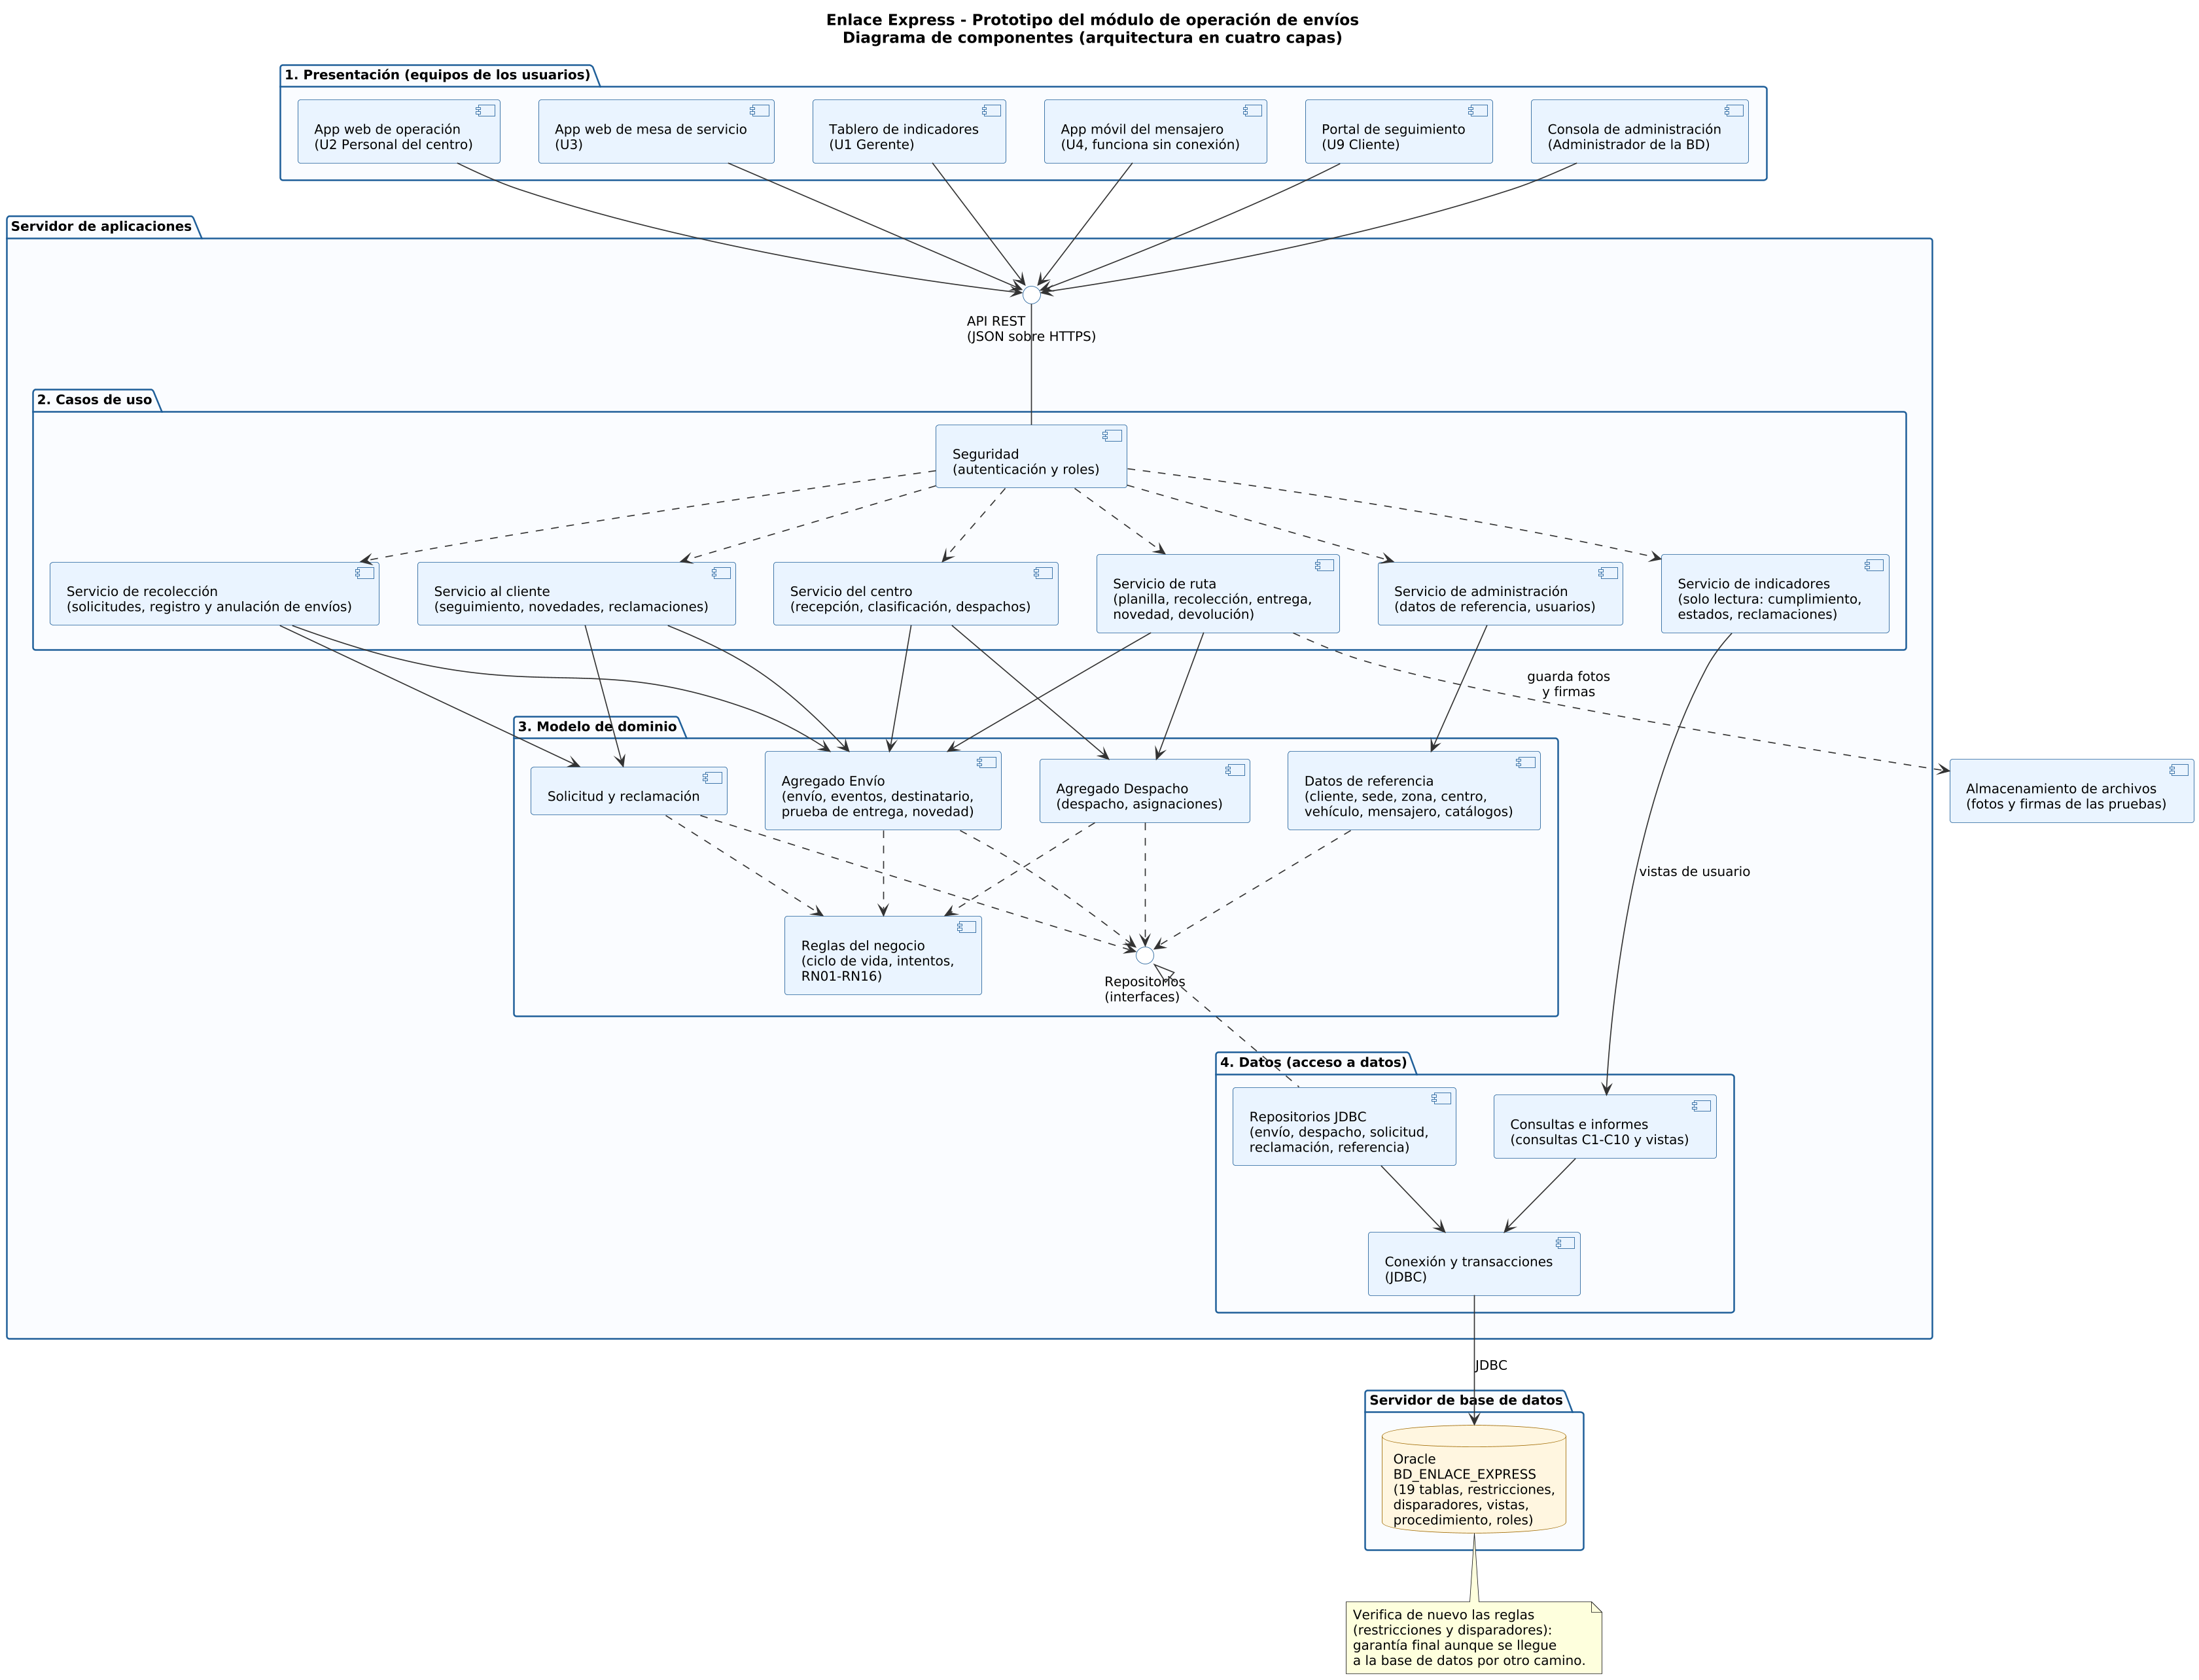
\includegraphics{figures/uml_componentes.png}}}
\caption{Diagrama de componentes del prototipo, en cuatro capas.}
\label{fig:proto-componentes}
\end{figure}

El diagrama de la figura~\ref{fig:proto-componentes} muestra la arquitectura
completa del diseño. El prototipo agrupa las aplicaciones de la capa de
presentación en una sola aplicación web con una sección por rol; no
implementa la aplicación móvil del mensajero con funcionamiento sin
conexión, la consola de administración ni el almacenamiento de fotos y
firmas, que están fuera del alcance (decisión A1).

\textbf{Casos de uso.} La figura~\ref{fig:proto-casos-uso-1} y la
figura~\ref{fig:proto-casos-uso-2} muestran el diagrama de casos de uso del
módulo, dividido en dos mitades para que se lea. La
tabla~\ref{tab:proto-cu} indica cuáles implementa el prototipo y cuál es
el servicio de la API de cada uno. Quedan fuera solo la gestión de datos de
referencia y de usuarios (CU27 y CU28), que la hace el administrador de la
base de datos con scripts, como dice el diseño, salvo el alta de cuentas de la
extensión E1. La gestión de novedades y de reclamaciones y la de centros y
zonas se probaron a nivel de base de datos en las transacciones T10 y T11
(subsección~\ref{sec:proto-transacciones}) y ahora también se hacen desde la
aplicación.

\begin{figure}[p]
\centering
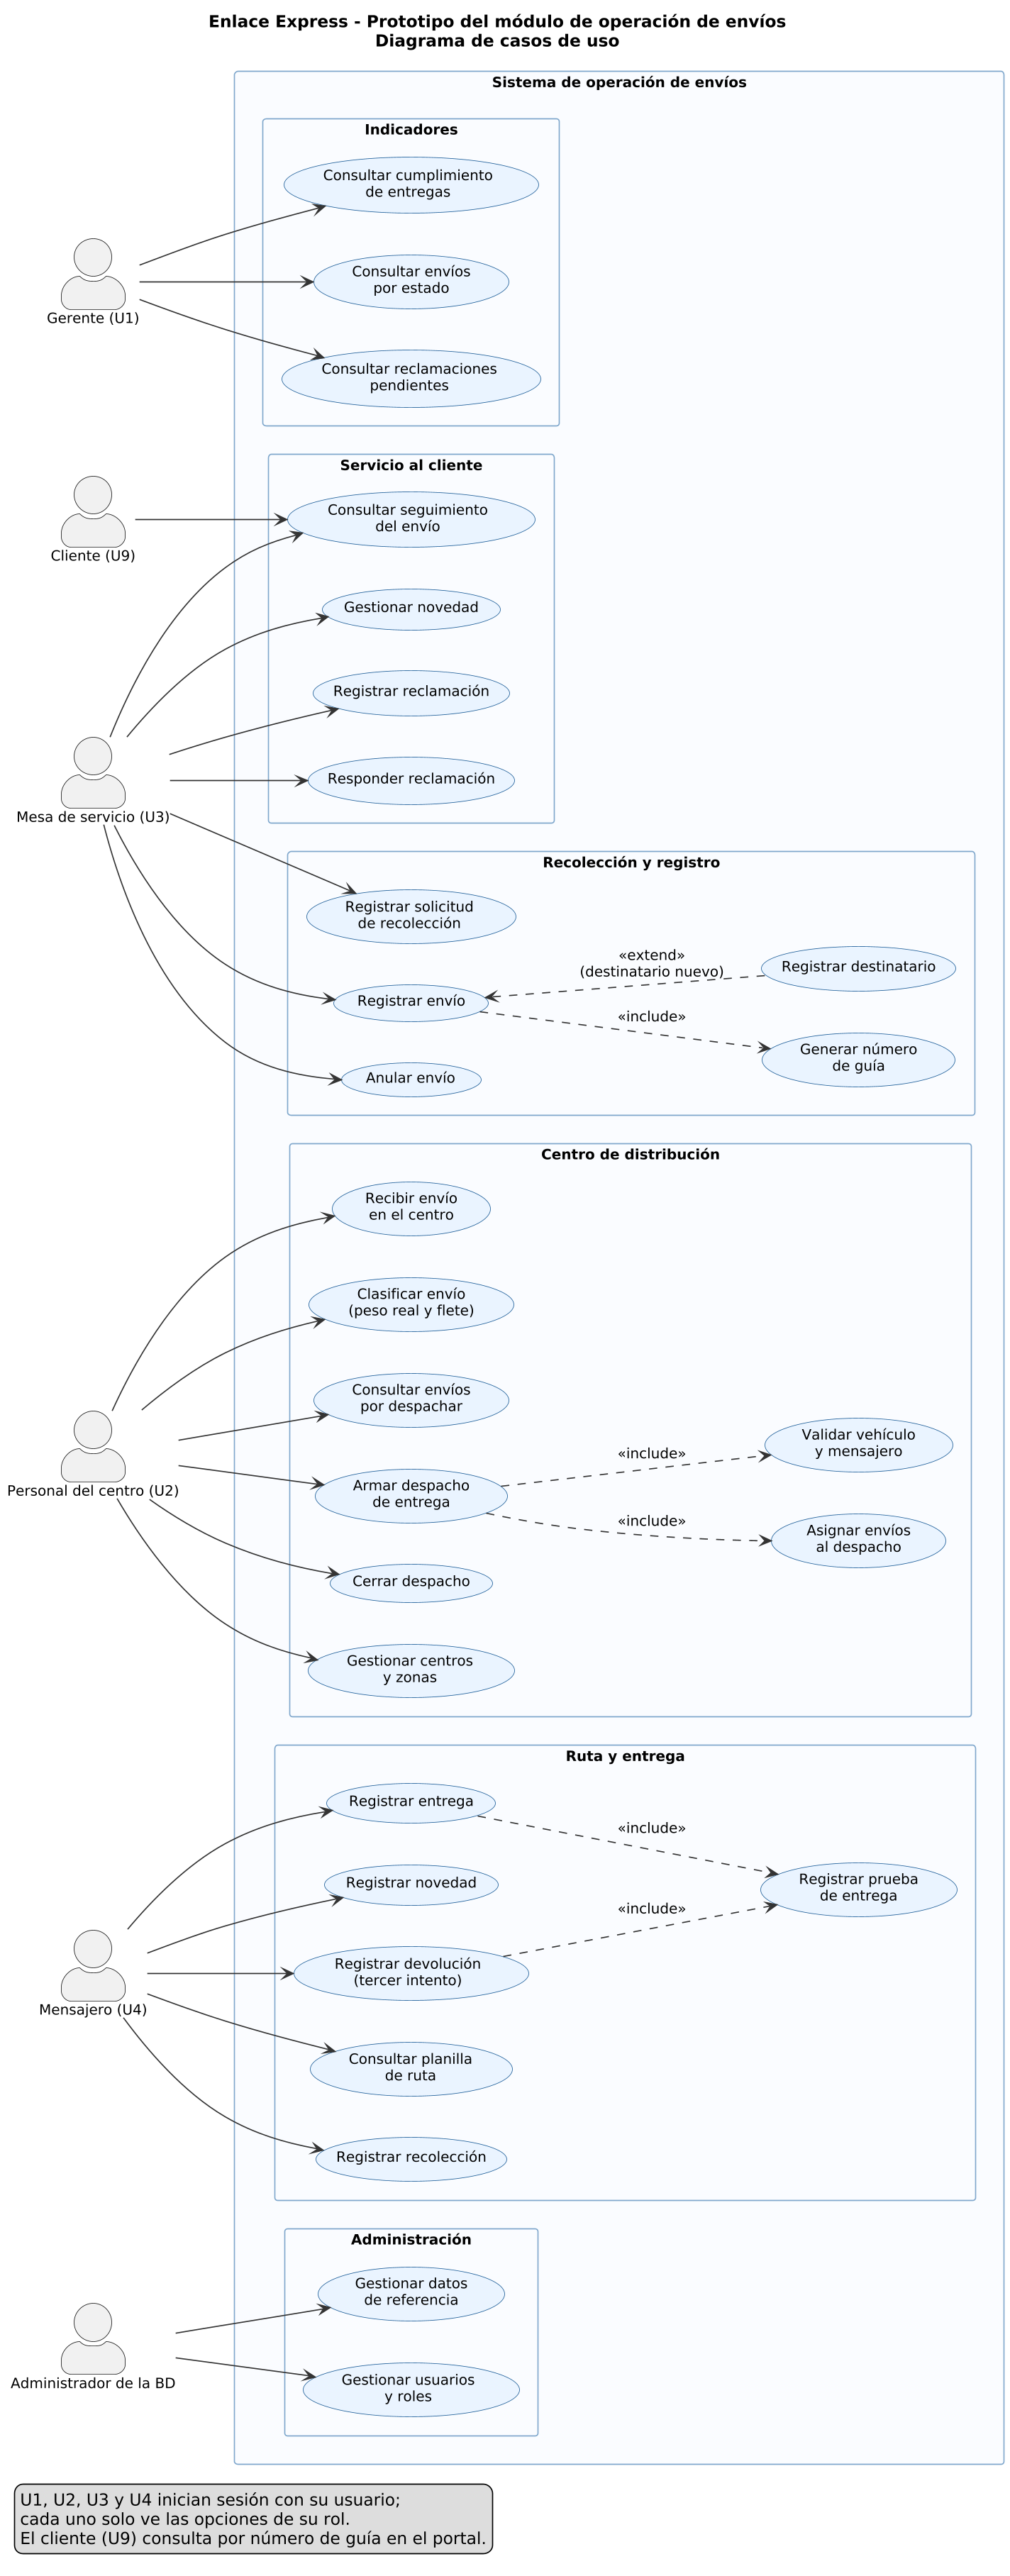
\includegraphics[trim=0 2023 0 0, clip, width=0.85\linewidth]{figures/uml_casos_uso.png}
\caption{Diagrama de casos de uso (primera parte): indicadores, servicio al cliente y recolección y registro.}
\label{fig:proto-casos-uso-1}
\end{figure}

\begin{figure}[p]
\centering
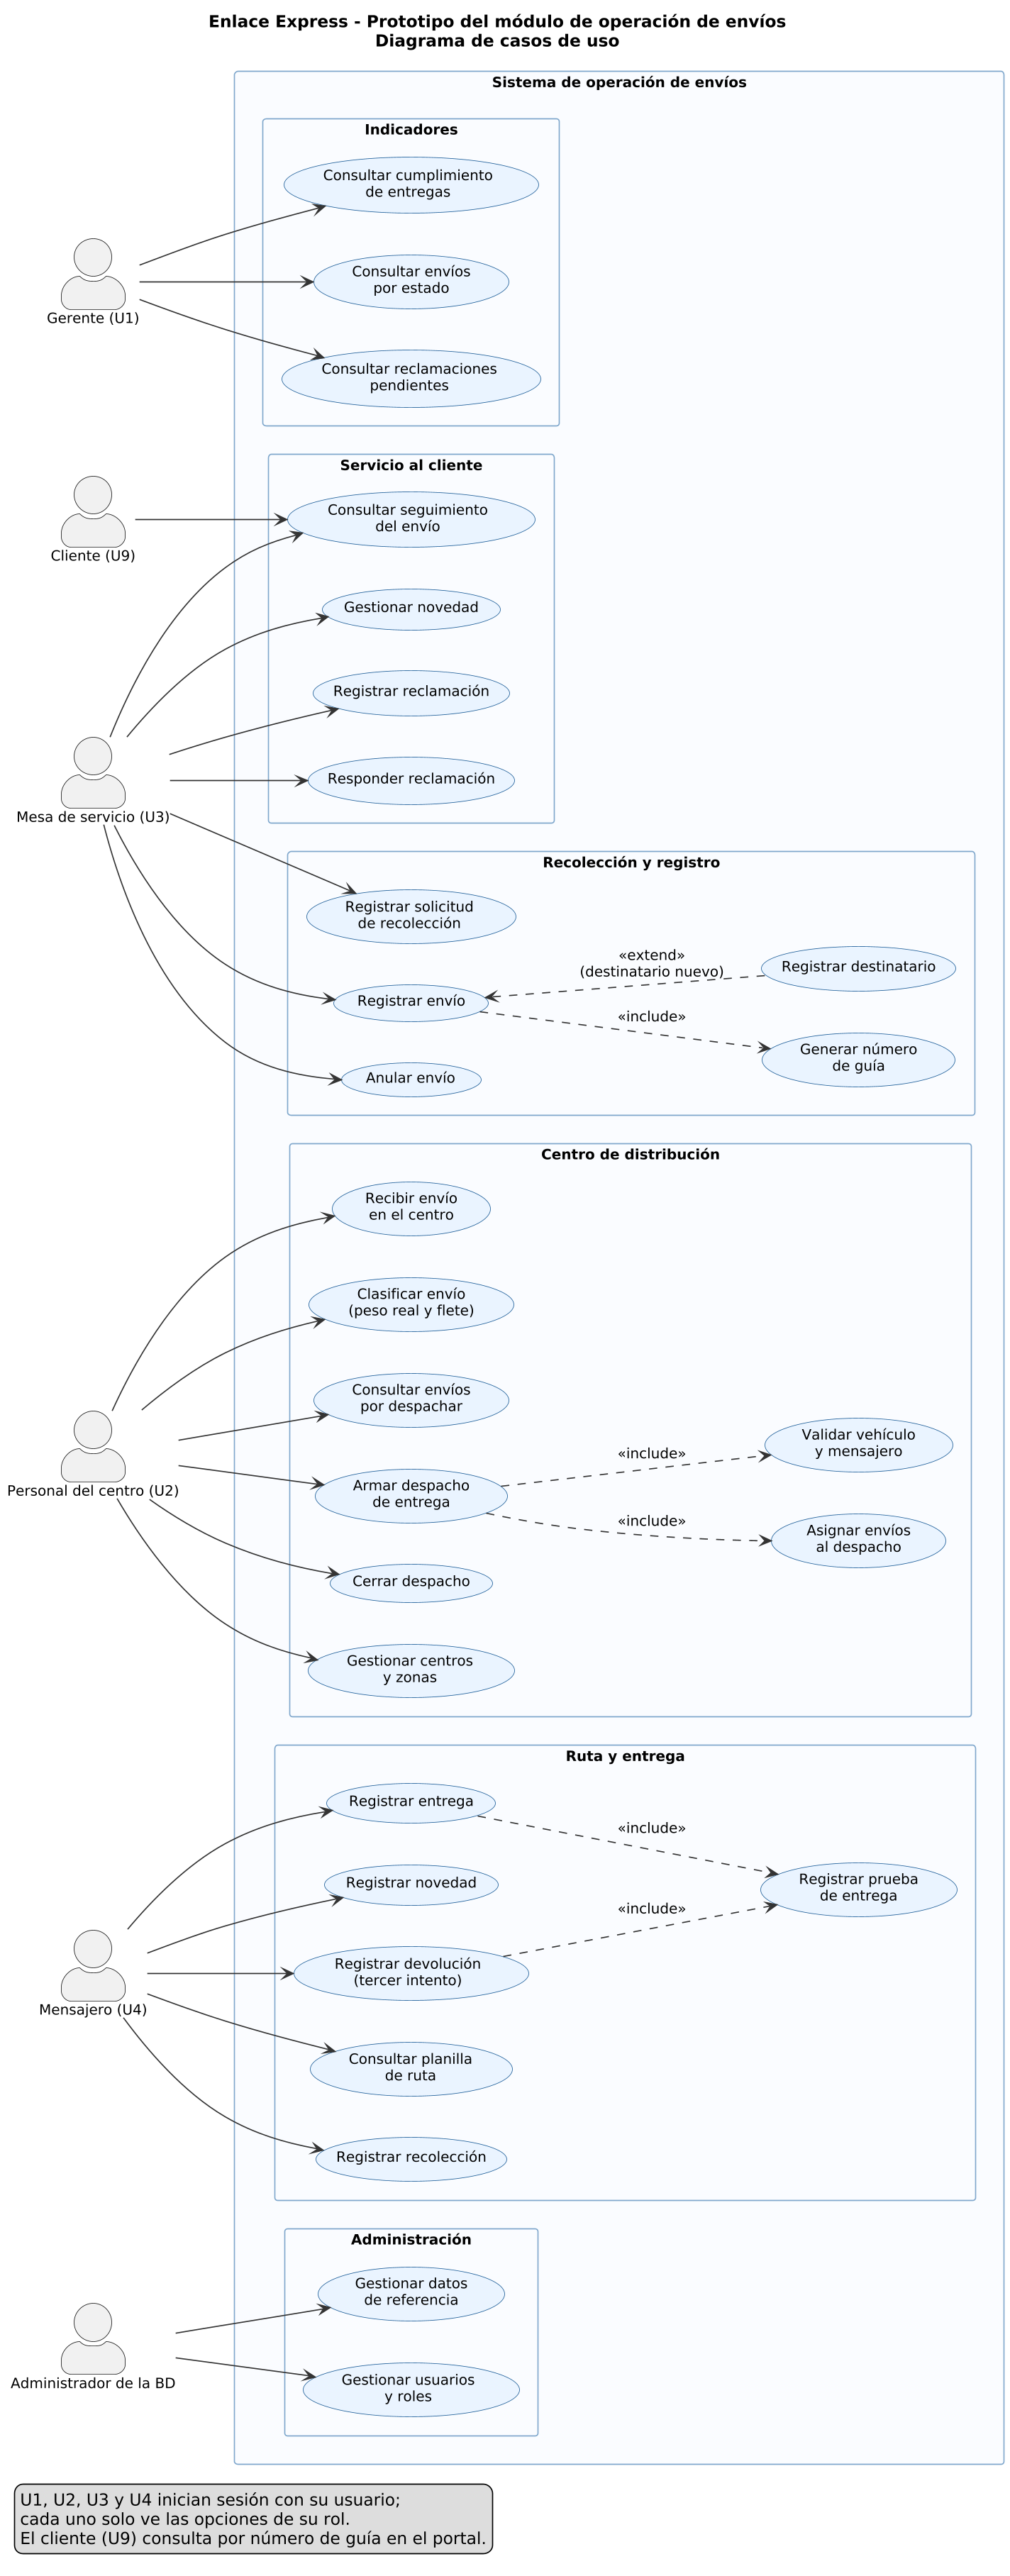
\includegraphics[trim=0 0 0 1609, clip, width=0.85\linewidth]{figures/uml_casos_uso.png}
\caption{Diagrama de casos de uso (segunda parte): centro de distribución, ruta y entrega, y administración.}
\label{fig:proto-casos-uso-2}
\end{figure}

{\singlespacing\footnotesize
\begin{longtable}{L{1.7cm} L{3.4cm} L{2.0cm} L{6.0cm}}
\caption{Casos de uso implementados por el prototipo y su servicio de la API.}
\label{tab:proto-cu}\\
\toprule
\textbf{Caso de uso} & \textbf{Nombre} & \textbf{Rol} & \textbf{Servicio de la API} \\
\midrule
\endfirsthead
\toprule
\textbf{Caso de uso} & \textbf{Nombre} & \textbf{Rol} & \textbf{Servicio de la API} \\
\midrule
\endhead
\bottomrule
\endfoot
CU01 & Registrar solicitud de recolección & Mesa & POST /api/\allowbreak{}mesa/\allowbreak{}solicitudes \\
CU02 a CU04 & Registrar envío (con número de guía y destinatario) & Mesa & POST /api/\allowbreak{}mesa/\allowbreak{}envios \\
CU05 & Anular envío & Mesa & POST /api/\allowbreak{}mesa/\allowbreak{}envios/\allowbreak{}\{guía\}/\allowbreak{}anular \\
CU06, CU07 & Recibir y clasificar envío & Centro & POST /api/\allowbreak{}centro/\allowbreak{}envios/\allowbreak{}\{guía\}/\allowbreak{}recepcion \\
CU08 & Consultar envíos por despachar & Centro & GET /api/\allowbreak{}centro/\allowbreak{}por-despachar \\
CU09 a CU11 & Armar despacho de entrega & Centro & POST /api/\allowbreak{}centro/\allowbreak{}despachos \\
CU12 & Cerrar despacho & Centro & POST /api/\allowbreak{}centro/\allowbreak{}despachos/\allowbreak{}\{id\}/\allowbreak{}cerrar \\
CU13 & Gestionar centros y zonas (sin borrar: el centro se inactiva) & Centro & GET y POST /api/\allowbreak{}centro/\allowbreak{}centros y /\allowbreak{}zonas; POST /api/\allowbreak{}centro/\allowbreak{}centros/\allowbreak{}\{id\}/\allowbreak{}modificar y /\allowbreak{}estado; POST /api/\allowbreak{}centro/\allowbreak{}zonas/\allowbreak{}\{id\}/\allowbreak{}modificar \\
CU14 & Consultar planilla de ruta & Mensajero, centro & GET /api/\allowbreak{}mensajero/\allowbreak{}planilla; GET /api/\allowbreak{}centro/\allowbreak{}despachos/\allowbreak{}\{id\}/\allowbreak{}planilla \\
CU15 & Registrar recolección & Mensajero & POST /api/\allowbreak{}mensajero/\allowbreak{}solicitudes/\allowbreak{}\{id\}/\allowbreak{}recolectar \\
CU16, CU19 & Registrar entrega con su prueba & Mensajero & POST /api/\allowbreak{}mensajero/\allowbreak{}asignaciones/\allowbreak{}\{id\}/\allowbreak{}entrega \\
CU17 & Registrar novedad & Mensajero & POST /api/\allowbreak{}mensajero/\allowbreak{}asignaciones/\allowbreak{}\{id\}/\allowbreak{}novedad \\
CU18 & Registrar devolución (tercer intento) & Mensajero & POST /api/\allowbreak{}mensajero/\allowbreak{}asignaciones/\allowbreak{}\{id\}/\allowbreak{}devolucion \\
CU20 & Consultar seguimiento del envío & Público, cliente, mesa & GET /api/\allowbreak{}publico/\allowbreak{}rastreo/\allowbreak{}\{guía\}; GET /api/\allowbreak{}cliente/\allowbreak{}envios/\allowbreak{}\{guía\}/\allowbreak{}seguimiento; GET /api/\allowbreak{}mesa/\allowbreak{}envios/\allowbreak{}\{guía\} \\
CU21 & Gestionar novedad (acción, solución y cierre) & Mesa & GET /api/\allowbreak{}mesa/\allowbreak{}novedades; POST /api/\allowbreak{}mesa/\allowbreak{}novedades/\allowbreak{}\{id\}/\allowbreak{}gestionar \\
CU22, CU23 & Registrar, responder y cerrar reclamaciones & Mesa & GET y POST /api/\allowbreak{}mesa/\allowbreak{}reclamaciones; POST /api/\allowbreak{}mesa/\allowbreak{}reclamaciones/\allowbreak{}\{id\}/\allowbreak{}responder y /\allowbreak{}cerrar \\
CU24 a CU26 & Consultar cumplimiento, envíos por estado y reclamaciones pendientes & Gerencia & GET /api/\allowbreak{}tablero/\allowbreak{}cumplimiento, /\allowbreak{}envios-por-estado y /\allowbreak{}reclamaciones-pendientes \\
\end{longtable}
\par}

La API está documentada con OpenAPI 3 y Swagger UI, que genera la
biblioteca springdoc a partir de los controladores: el documento se entrega
en \texttt{/v3/api-docs} y la interfaz en \texttt{/swagger-ui.html}, ambos sin
sesión y de solo lectura. Las rutas se agrupan por sección, cada una indica el
rol que exige, y el documento describe la sesión por cookie, el token CSRF y el
formato de los errores (Problem Details con la propiedad \texttt{codigo}). El
documento generado se guardó en \texttt{docs/evidence/13\_openapi.json} y una
captura de la interfaz en \texttt{docs/evidence/13\_swagger\_ui.png}.

\textbf{Dominio y acceso a datos.} Las figuras~\ref{fig:proto-clases-dominio}
y~\ref{fig:proto-clases-mapeadores} muestran las clases del modelo de dominio
y de los mapeadores. Los datos se leen y guardan con el patrón Data Mapper, sin
ORM: cada mapeador es una clase con el SQL de sus operaciones escrito como
constantes y ejecutado con \texttt{PreparedStatement} y variables de enlace.
Los valores nunca se concatenan en el SQL. El siguiente extracto de
\texttt{EnvioMapper} muestra el SQL que inserta un evento y el que bloquea la fila
de un envío, con el método que guarda el evento.

\begin{figure}[p]
\centering
\rotatebox{90}{\adjustbox{max width=0.95\textheight, max height=0.98\linewidth}{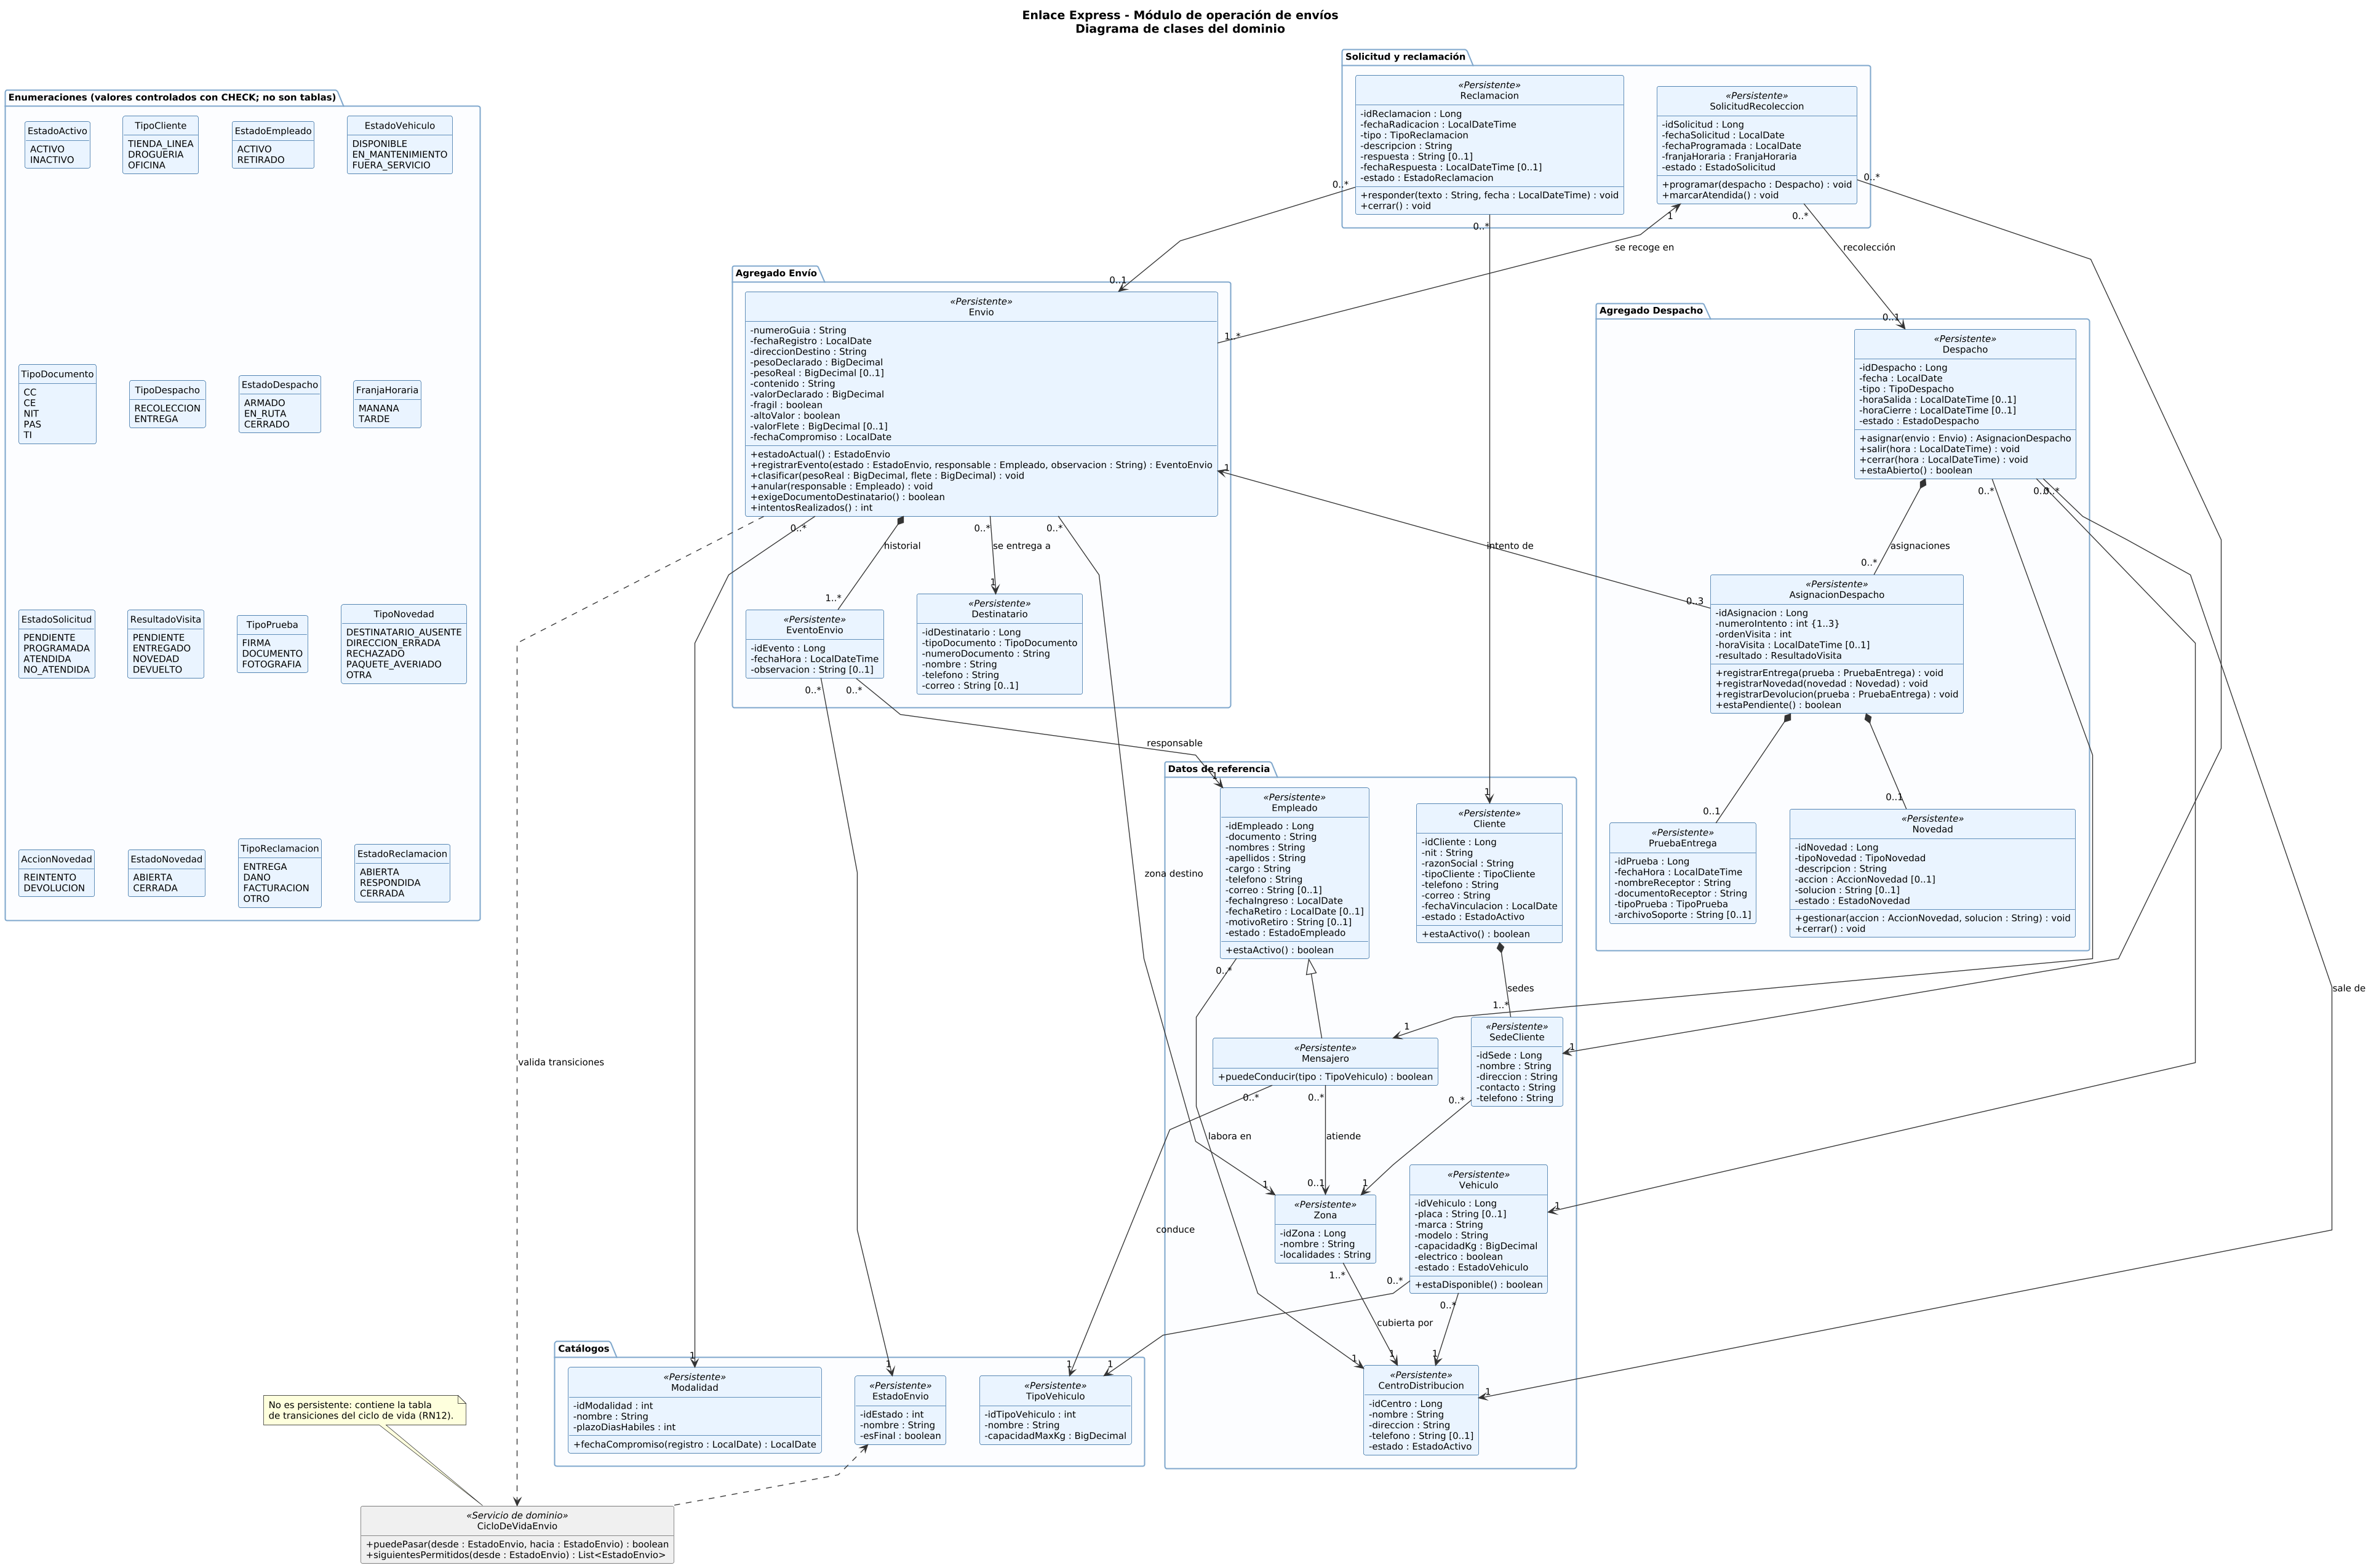
\includegraphics{figures/uml_clases_dominio.png}}}
\caption{Diagrama de clases del modelo de dominio.}
\label{fig:proto-clases-dominio}
\end{figure}

\begin{figure}[p]
\centering
\rotatebox{90}{\adjustbox{max width=0.95\textheight, max height=0.98\linewidth}{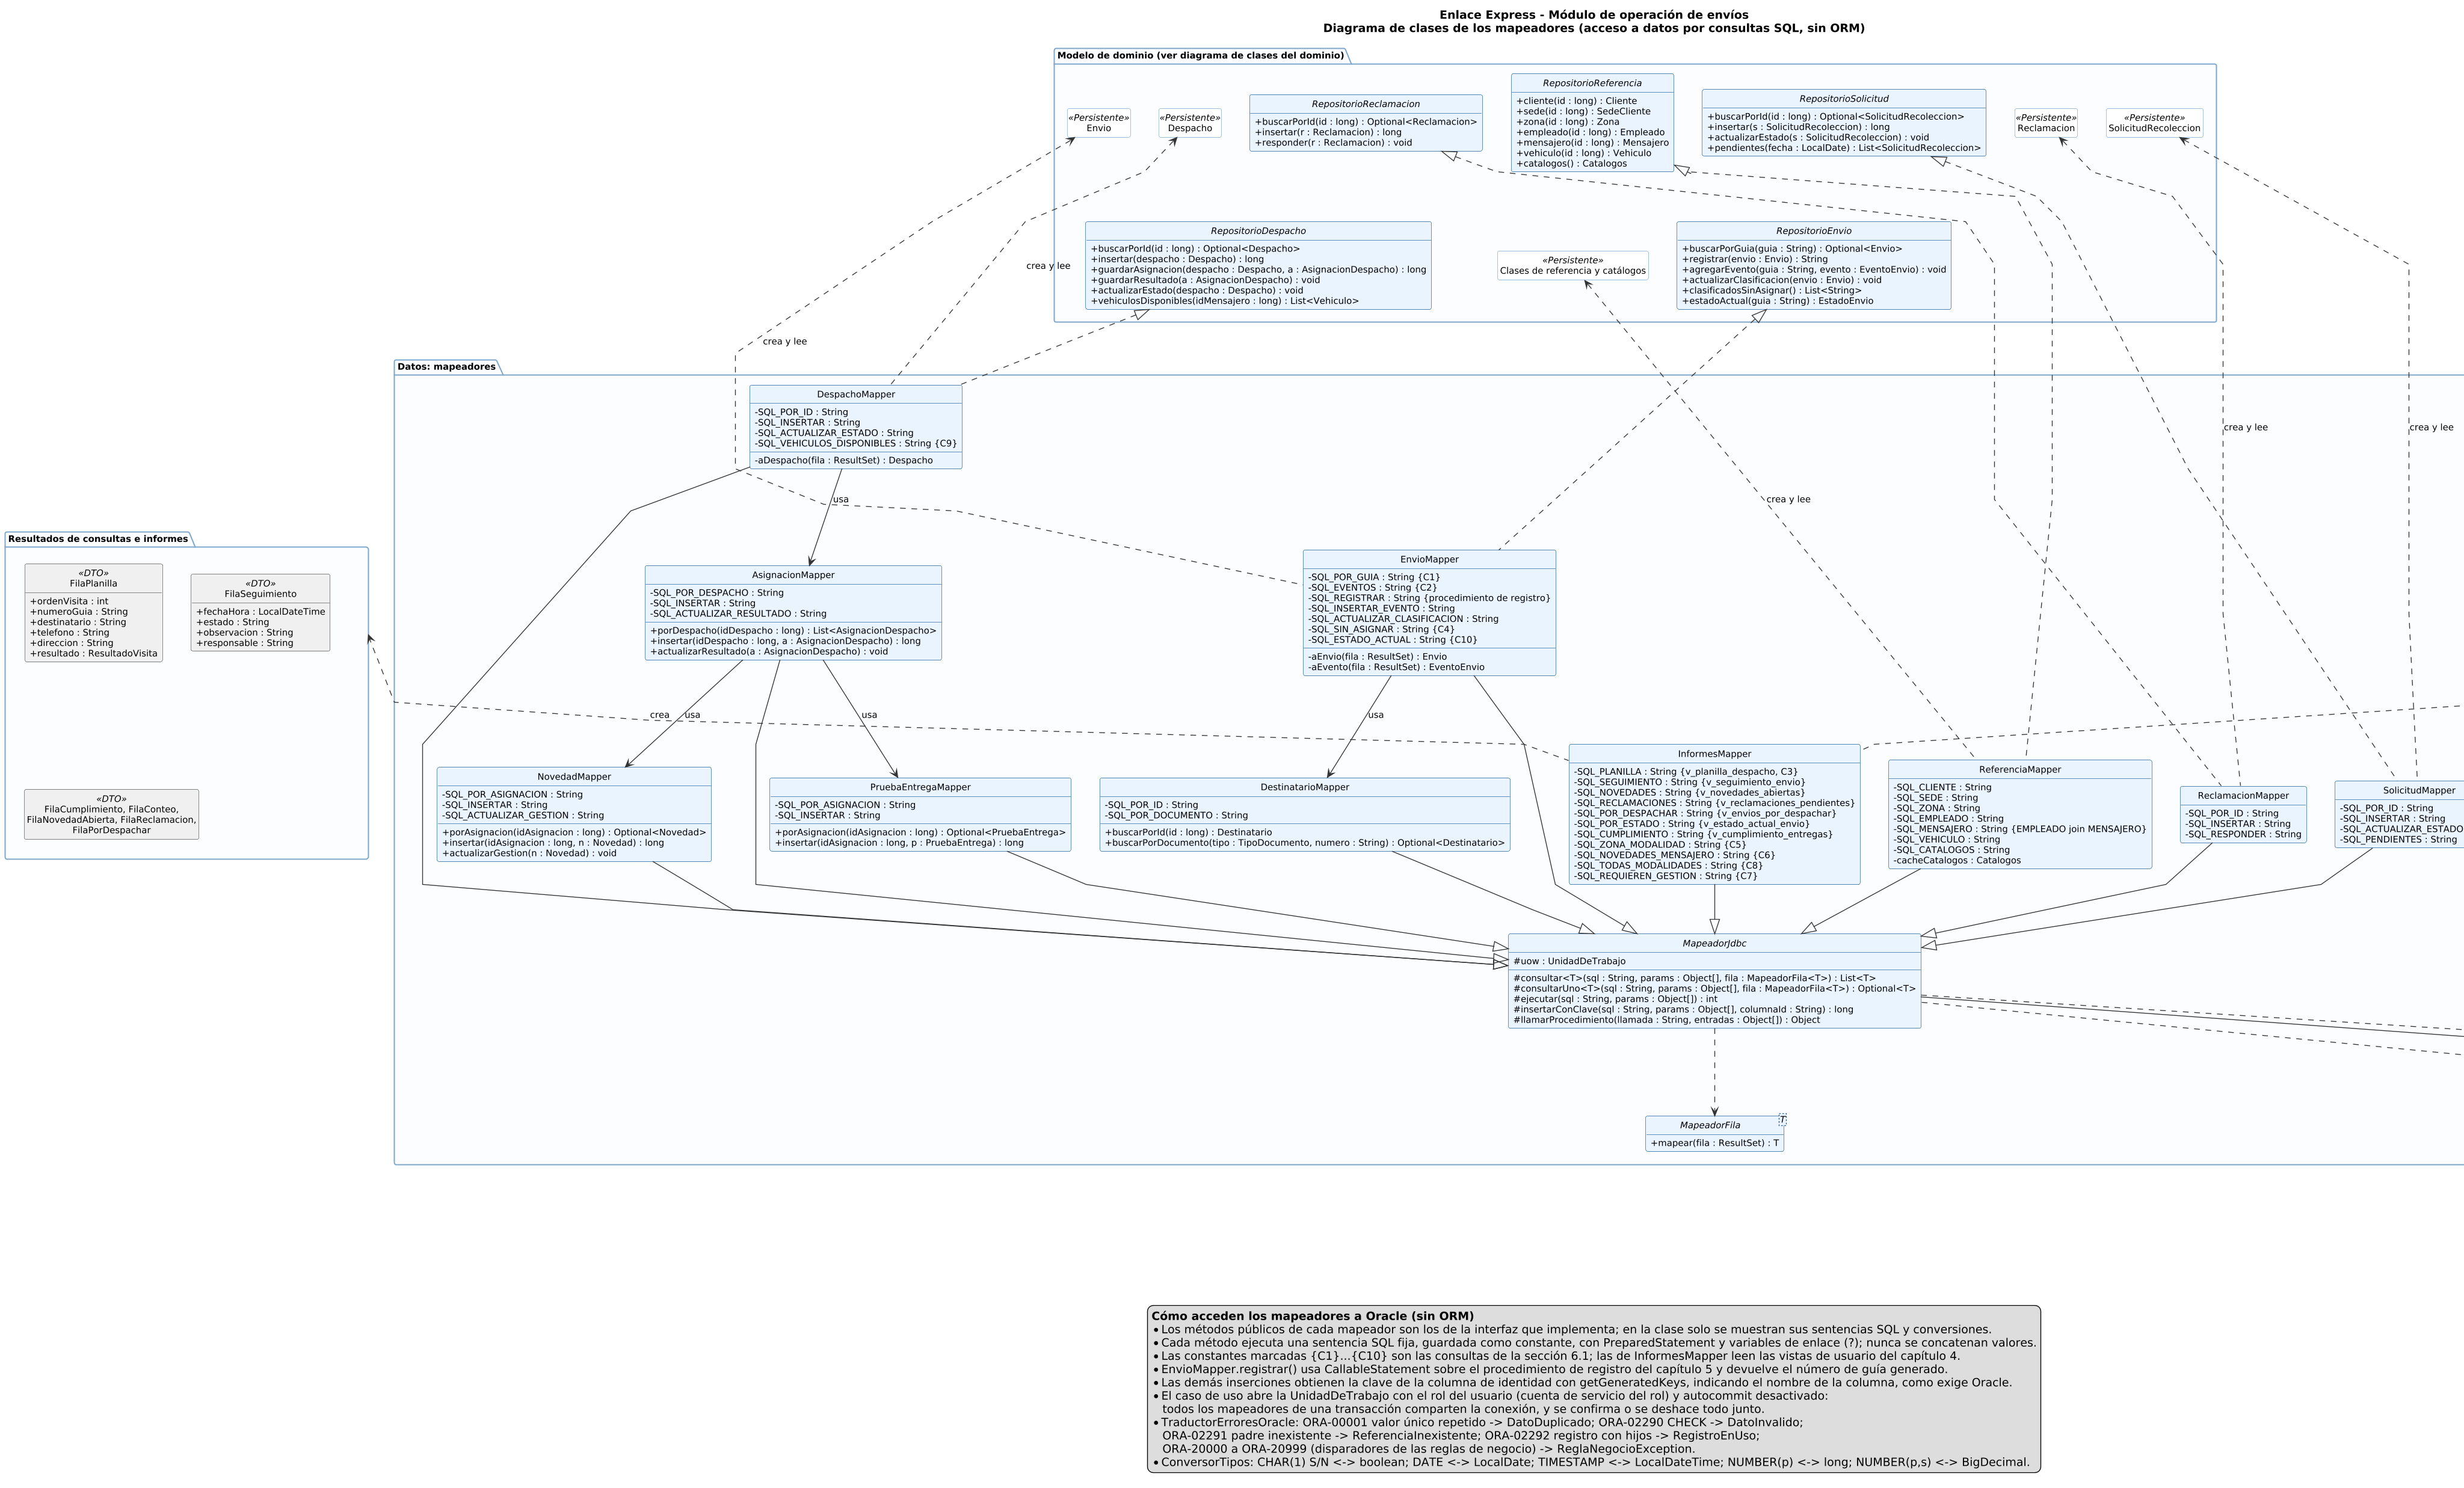
\includegraphics{figures/uml_clases_mapeadores.png}}}
\caption{Diagrama de clases de los mapeadores (Data Mapper sin ORM).}
\label{fig:proto-clases-mapeadores}
\end{figure}

% Los renglones del extracto se acomodaron para que quepan en la pagina.
\begin{lstlisting}[style=sqlpro,language=Java]
private static final String SQL_INSERTAR_EVENTO = """
    INSERT INTO evento_envio (numero_guia, id_estado,
           id_empleado, fecha_hora, observacion)
    VALUES (?, ?, ?, ?, ?)""";

private static final String SQL_BLOQUEAR =
    "SELECT numero_guia FROM envio WHERE numero_guia = ? FOR UPDATE";

public void agregarEvento(String numeroGuia, EventoEnvio evento) {
    long id = insertarConClave(SQL_INSERTAR_EVENTO,
        new Object[] {numeroGuia, evento.estado().idEstado(),
            evento.idEmpleado(), evento.fechaHora(),
            evento.observacion()}, "ID_EVENTO");
    evento.asignarId(id);
}
\end{lstlisting}

Tres clases de la infraestructura sostienen a los mapeadores:

\begin{itemize}[itemsep=2pt]
  \item \textbf{\texttt{UnidadDeTrabajo}} es una transacción: una conexión de
        la cuenta de servicio del rol, sin confirmación automática, que
        comparten todos los mapeadores de un caso de uso. Se confirma o se
        deshace todo junto, sin \texttt{@Transactional}: el caso de uso la
        abre al empezar, llama a \texttt{confirmar} al final y, si
        falla antes, al cerrarla se deshace sola.
  \item \textbf{\texttt{FabricaConexiones}} mantiene un pequeño grupo de
        conexiones por cuenta de servicio, una por rol. Cada conexión nueva
        fija el esquema BD\_ENLACE\_EXPRESS y la zona horaria America/Bogota,
        de modo que el SQL es el mismo de la sección~\ref{sec:algebra}.
  \item \textbf{\texttt{TraductorErroresOracle}} convierte los errores de
        Oracle en excepciones del dominio, que la API responde con un código HTTP
        y el formato de errores estándar Problem Details, con la propiedad
        \texttt{codigo}. La tabla~\ref{tab:proto-errores} resume la
        conversión.
\end{itemize}

{\singlespacing\small
\begin{longtable}{L{4.8cm} L{1.4cm} L{5.4cm}}
\caption{Conversión de errores de Oracle a respuestas de la API.}
\label{tab:proto-errores}\\
\toprule
\textbf{Error de Oracle} & \textbf{HTTP} & \textbf{Código de la respuesta} \\
\midrule
\endfirsthead
\toprule
\textbf{Error de Oracle} & \textbf{HTTP} & \textbf{Código de la respuesta} \\
\midrule
\endhead
\bottomrule
\endfoot
ORA-20000 a ORA-20999 (reglas de negocio y E1) & 422 & El de la regla: RN07, E1, etc. \\
ORA-02290, ORA-01400, ORA-12899 (CHECK, NOT NULL, longitud) & 400 & DATO\_INVALIDO \\
ORA-02291 (clave foránea inexistente) & 400 & REFERENCIA\_INEXISTENTE \\
ORA-00001 (UNIQUE) & 409 & DATO\_DUPLICADO \\
ORA-02292 (registro con dependientes) & 409 & REGISTRO\_EN\_USO \\
ORA-00054 (recurso ocupado) & 409 & RECURSO\_OCUPADO \\
ORA-00942, ORA-01031, ORA-41900 (privilegio) & 403 & ACCESO\_DENEGADO \\
Cualquier otro & 500 & ERROR\_INTERNO, sin detalles de la base \\
\end{longtable}
\par}

\textbf{Reglas en dos niveles.} Las reglas de negocio se verifican primero en el
dominio, con el mismo código y el mismo texto que usa Oracle, y la base de
datos las vuelve a verificar como garantía final. La regla RN12 muestra los
dos niveles. En el dominio, \texttt{CicloDeVidaEnvio} rechaza una
transición no permitida con el código RN12 y la prueba unitaria
\texttt{CicloDeVidaEnvioTest} lo comprueba. En la base de datos, el disparador
\texttt{trg\_evento\_transicion} rechaza la misma transición con ORA-20012,
que probaron las transacciones (T3 a T7 y T12,
tabla~\ref{tab:proto-casos}). Para el usuario, ambos dan el mensaje que
aparece en la figura~\ref{fig:proto-rn12}, que empieza por el código de la
regla.

\textbf{Seguridad.} El acceso sigue tres pasos: el rol de la aplicación del
usuario que inició sesión decide qué servicios puede llamar; el servidor elige
entonces la cuenta de servicio de ese rol; y la base de datos limita lo que esa
cuenta puede hacer con los permisos del capítulo~5.

\begin{itemize}[itemsep=2pt]
  \item \textbf{Sesión y contraseñas.} La sesión vive en el servidor y el
        navegador solo guarda una cookie, protegida contra el acceso desde
        scripts y con la restricción \texttt{SameSite}. Las contraseñas se
        guardan con BCrypt. Una contraseña débil o un dato faltante se
        rechazan, y un usuario o una contraseña incorrectos dan siempre el
        mismo mensaje.
  \item \textbf{CSRF.} Las operaciones que cambian datos exigen un
        token contra falsificación de peticiones (CSRF), que el navegador
        devuelve en un encabezado.
  \item \textbf{Registro con código (E1).} Un empleado o un cliente se
        registra con su documento o NIT y un código de activación de un solo
        uso, y el rol lo deriva la base de datos del cargo
        (subsección~\ref{sec:proto-extensiones}).
  \item \textbf{Identificador de cliente.} Cada transacción fija, con el
        nombre del usuario, el identificador de cliente de la sesión de Oracle
        (decisión A2). El script
        \texttt{test-client-identifier.sh} lo comprobó
        con la auditoría unificada de Oracle: \texttt{demo\_mesa} registró una
        solicitud y un envío por la API, y la auditoría guardó su nombre como
        identificador de cliente aunque la conexión es de la cuenta
        \texttt{svc\_mesa} (tabla~\ref{tab:proto-auditoria}).
  \item \textbf{Rastreo público (E2).} Cualquiera consulta un envío por su
        número de guía, sin cuenta, y ve solo fecha, estado y zona de cada
        evento. La aplicación limita las consultas por dirección IP, y la
        prueba de integración \texttt{SeguridadIT} comprueba que la consulta
        número 31 dentro de un minuto recibe el estado 429.
\end{itemize}

% Fuente: docs/evidence/11_identificador_cliente.txt
{\singlespacing\small
\begin{longtable}{L{2.8cm} L{2.2cm} L{2.8cm} L{2.2cm} L{3.6cm}}
\caption{Auditoría de Oracle de una operación hecha por la aplicación con el usuario demo\_mesa.}
\label{tab:proto-auditoria}\\
\toprule
\textbf{Hora} & \textbf{Cuenta de la base} & \textbf{Identificador de cliente} & \textbf{Acción} & \textbf{Objeto} \\
\midrule
\endfirsthead
\toprule
\textbf{Hora} & \textbf{Cuenta de la base} & \textbf{Identificador de cliente} & \textbf{Acción} & \textbf{Objeto} \\
\midrule
\endhead
\bottomrule
\endfoot
21/11/2026 16:55:31 & SVC\_MESA & demo\_mesa & INSERT & SOLICITUD\_\allowbreak RECOLECCION \\
21/11/2026 16:55:31 & SVC\_MESA & demo\_mesa & EXECUTE & PR\_REGISTRAR\_\allowbreak ENVIO \\
\end{longtable}
\par}

\textbf{Flujo principal.} El flujo principal definido para el prototipo es: registrar
el envío, recolectarlo, recibirlo y clasificarlo, armar el despacho,
entregar con prueba y consultar el seguimiento público; después, un caso
de rechazo con la devolución en el tercer intento y una transición bloqueada.
La prueba de punta a punta, que se describe al final de esta subsección,
lo recorre en el navegador con los usuarios de demostración y guardó una
captura de cada paso; las que siguen son las principales. Los envíos del
recorrido son EE0000000000030, el frágil, y EE0000000000031, el que termina
devuelto.

El rastreo público (figura~\ref{fig:proto-rastreo}) es la pantalla de inicio y
no pide sesión: muestra el estado actual y la línea de tiempo del envío.

\begin{figure}[htbp]
\centering
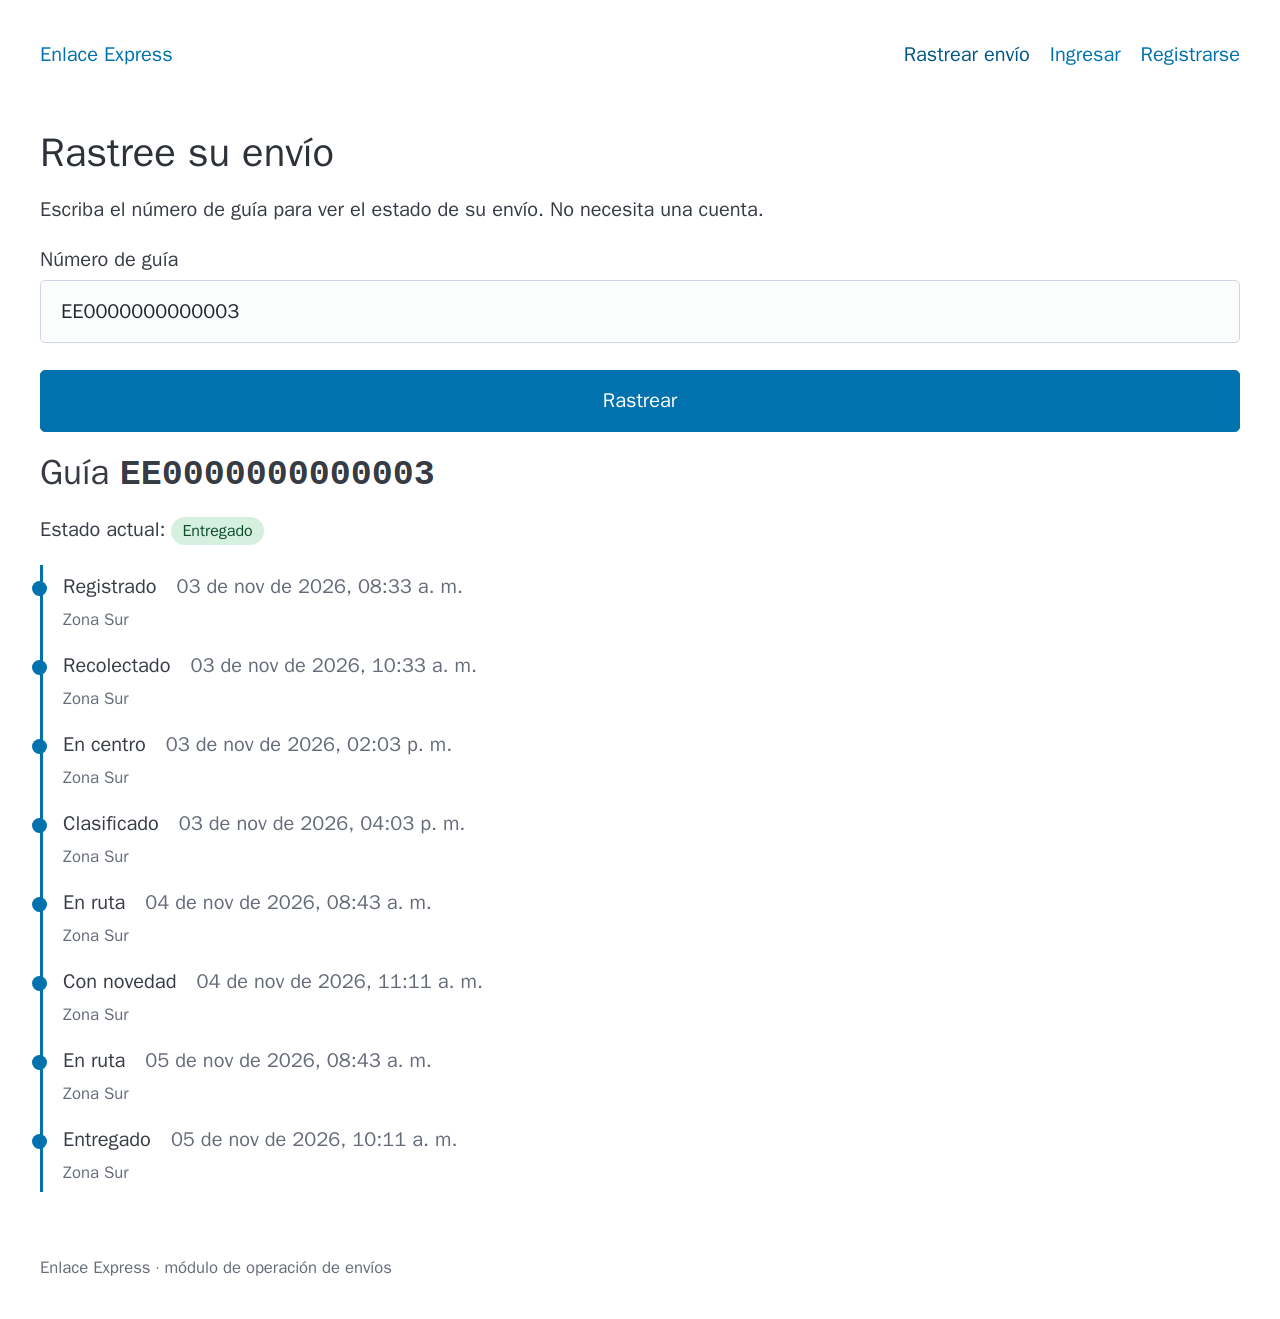
\includegraphics[width=0.6\linewidth]{figures/01_rastreo_publico.png}
\caption{Rastreo público de la guía EE0000000000003: estado actual y recorrido con fecha, estado y zona, sin datos personales.}
\label{fig:proto-rastreo}
\end{figure}

La mesa de servicio, después de iniciar sesión, registra la solicitud de
recolección del cliente y luego los envíos, uno frágil y uno normal. Al
registrar un envío, la aplicación muestra el número de guía que genera
la base de datos y la fecha de compromiso que calcula con la modalidad
(figura~\ref{fig:proto-registro}).

\begin{figure}[htbp]
\centering
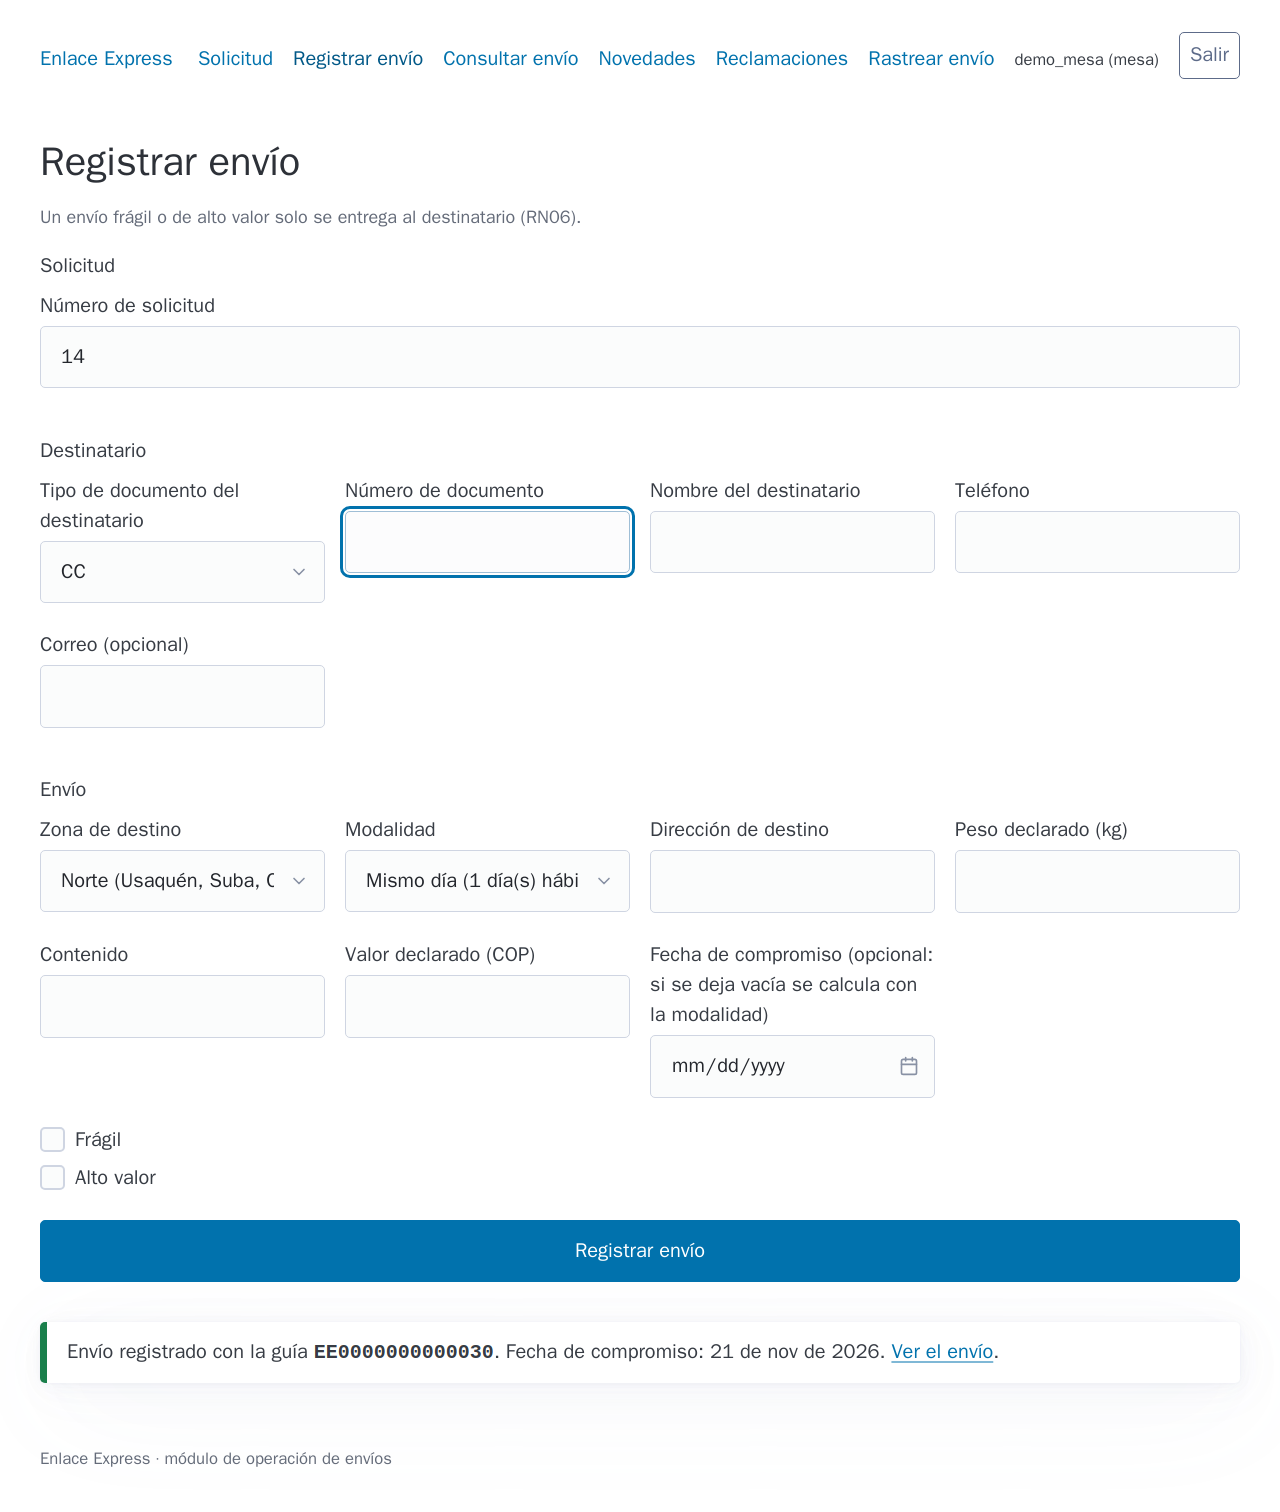
\includegraphics[trim=0 70 0 0, clip, width=0.6\linewidth]{figures/04_mesa_registro_envio.png}
\caption{Registro de un envío por la mesa de servicio: el mensaje de éxito muestra la guía y la fecha de compromiso.}
\label{fig:proto-registro}
\end{figure}

El mensajero recolecta la solicitud, y el centro recibe cada envío con su peso
real y su flete (figura~\ref{fig:proto-recepcion}), que quedan clasificados. Luego
el centro arma el despacho de entrega: elige los envíos clasificados, un
mensajero y uno de los vehículos disponibles de su tipo, y la aplicación
informa el número de despacho (figura~\ref{fig:proto-despacho}).

\begin{figure}[htbp]
\centering
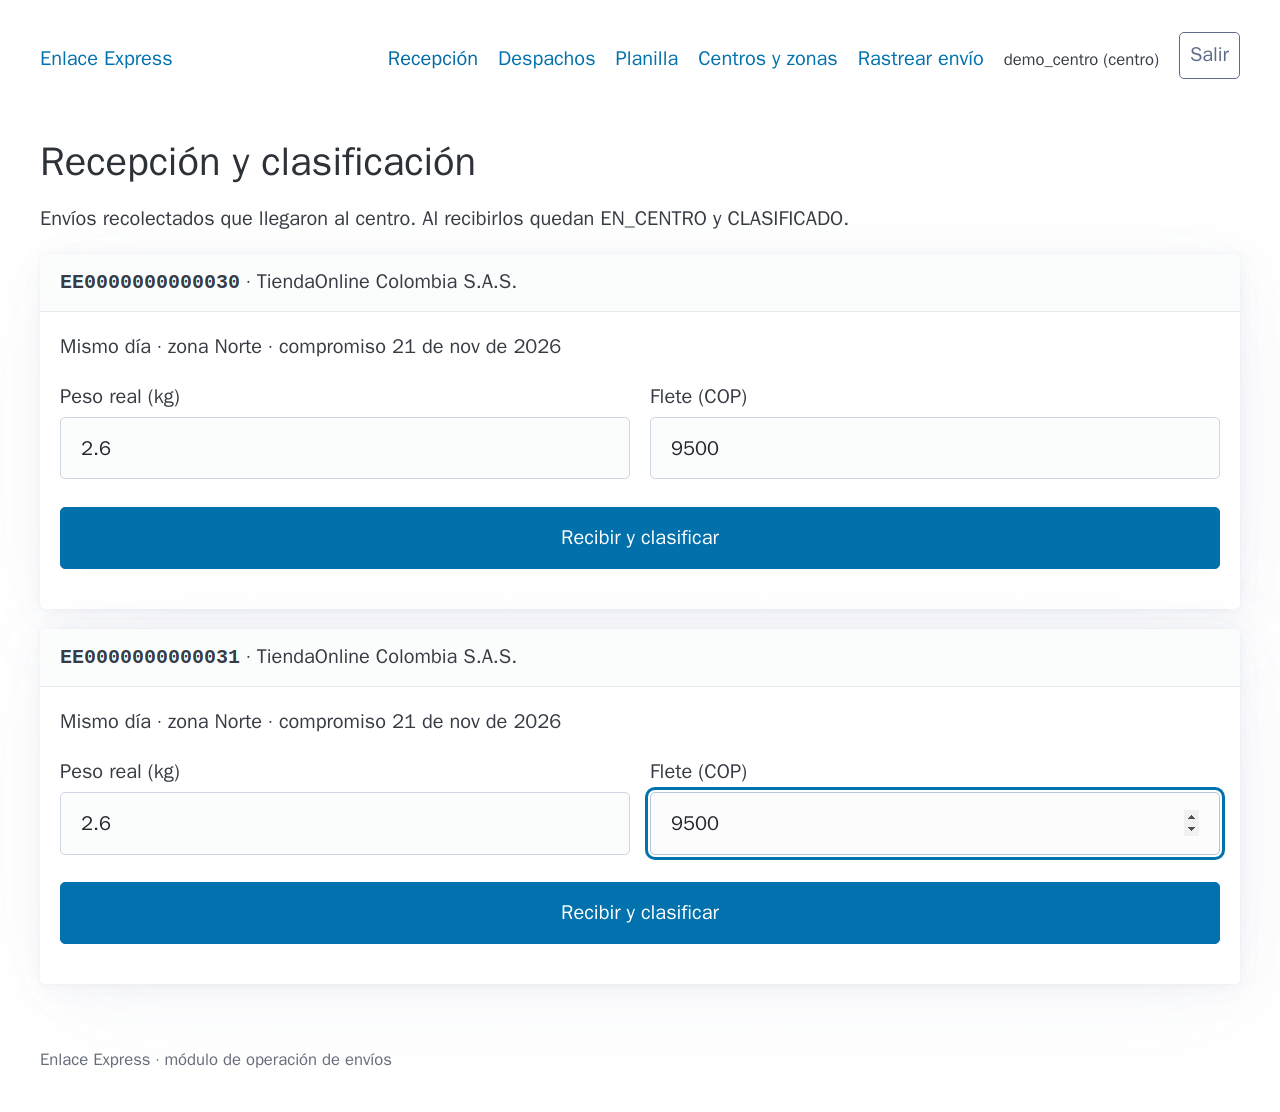
\includegraphics[width=0.75\linewidth]{figures/06_centro_recepcion.png}
\caption{Recepción y clasificación en el centro: peso real y flete de cada envío recolectado.}
\label{fig:proto-recepcion}
\end{figure}

\begin{figure}[htbp]
\centering
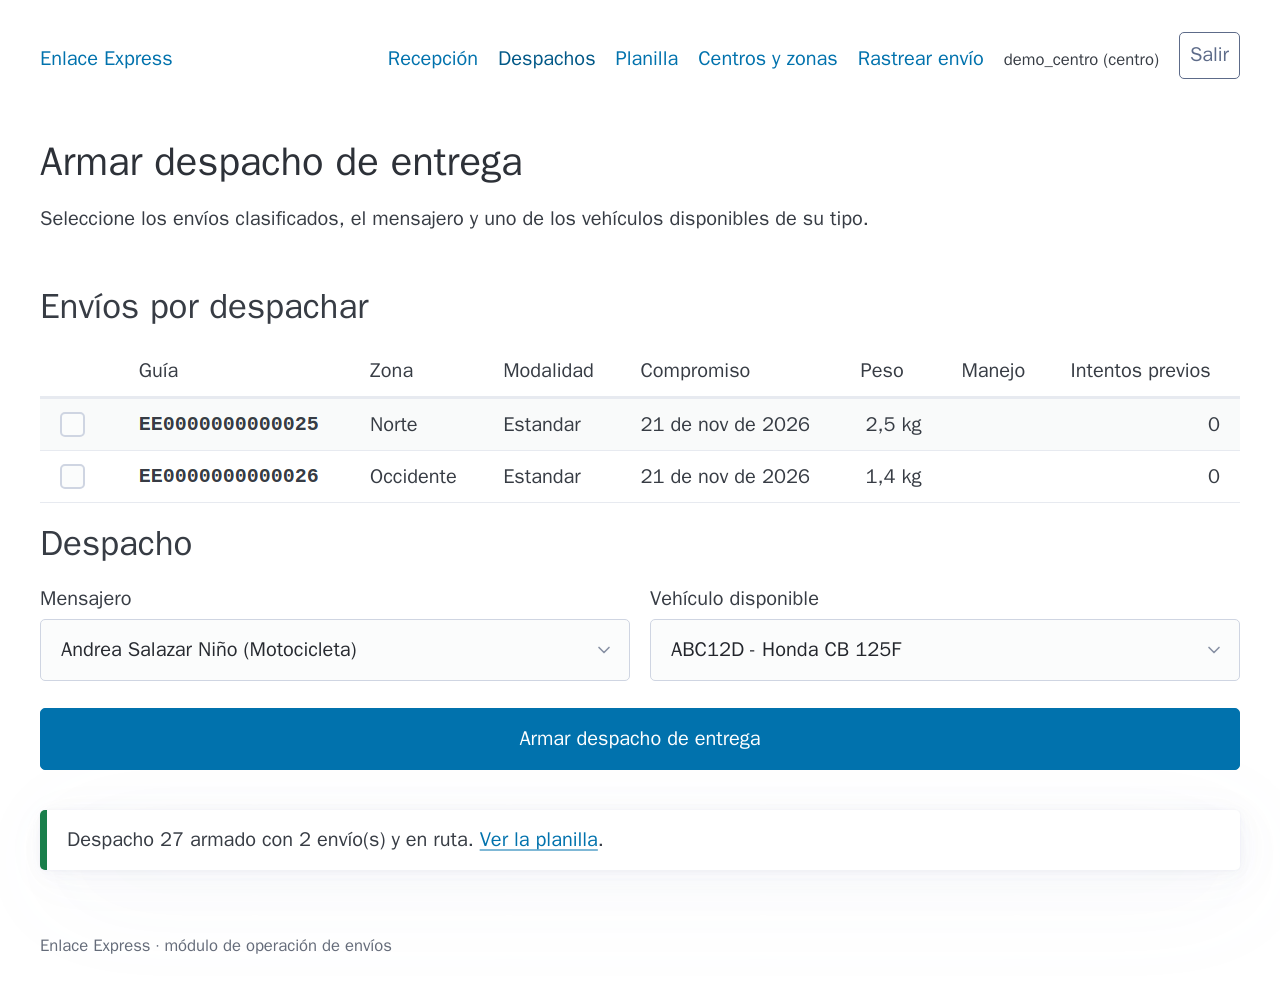
\includegraphics[width=0.75\linewidth]{figures/07_centro_despacho_armado.png}
\caption{Despacho armado por el centro, con el aviso del número de despacho.}
\label{fig:proto-despacho}
\end{figure}

La planilla del mensajero se diseñó para el teléfono: una columna, botones
grandes y el envío frágil resaltado, con la indicación de que solo se
entrega al destinatario. En la figura~\ref{fig:proto-movil} el mensajero intenta
entregar el envío frágil con el documento de otra persona y el sistema rechaza la
entrega con el mensaje de la regla RN06; con el documento del destinatario
la entrega se acepta.

\begin{figure}[htbp]
\centering
\begin{minipage}[t]{0.40\linewidth}
\centering
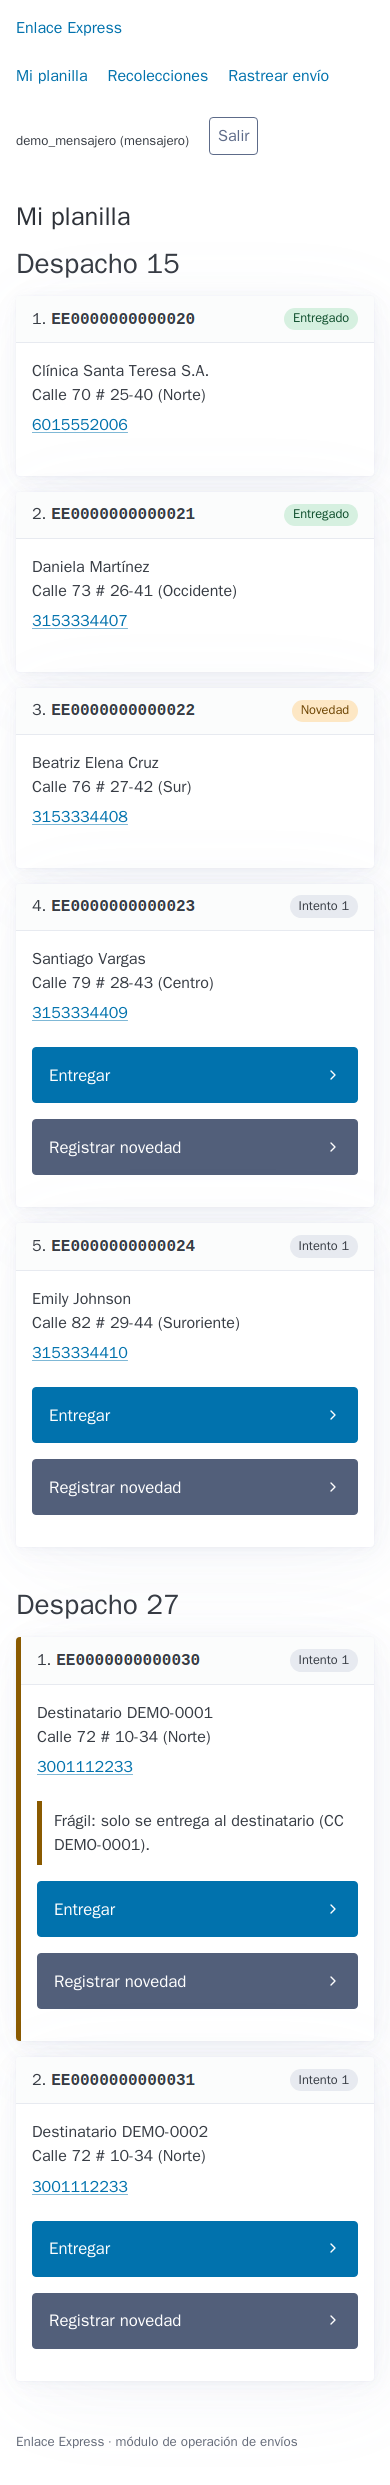
\includegraphics[trim=0 385 0 1560, clip, width=\linewidth]{figures/09_mensajero_planilla_movil.png}
\end{minipage}\hfill
\begin{minipage}[t]{0.40\linewidth}
\centering
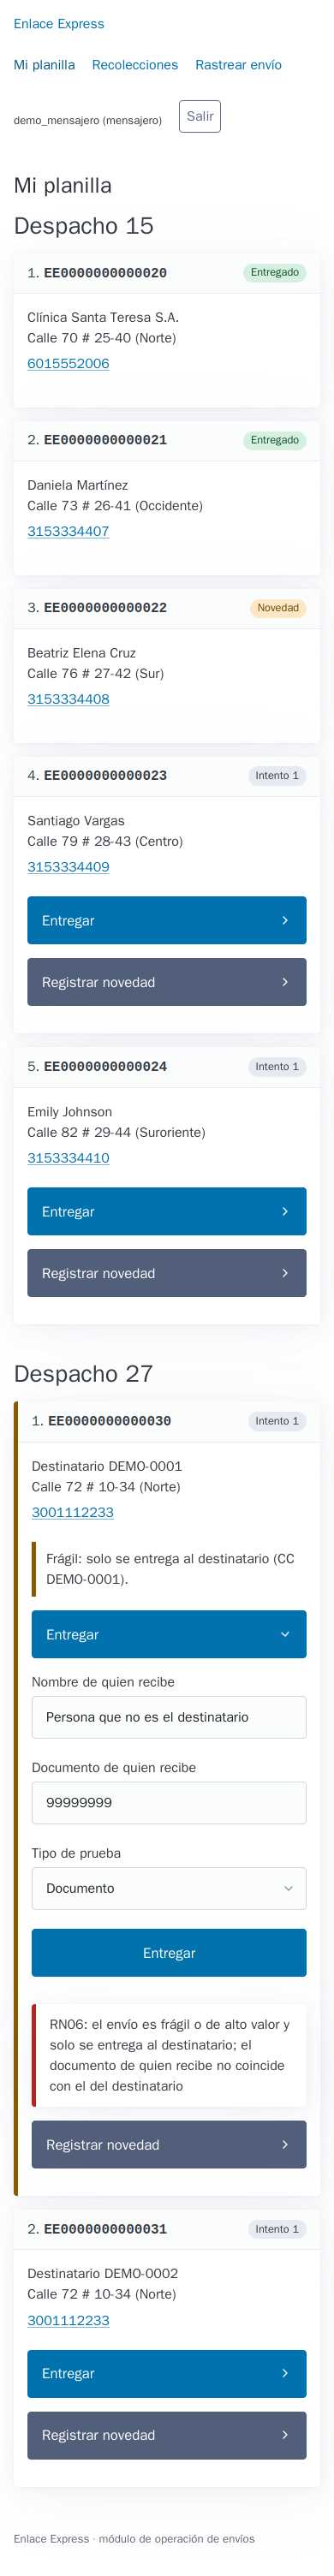
\includegraphics[trim=0 409 0 1590, clip, width=\linewidth]{figures/10_rechazo_rn06_movil.png}
\end{minipage}
\caption{Planilla del mensajero en el teléfono, con el envío frágil resaltado (izquierda), y rechazo RN06 al intentar entregarlo con el documento de otra persona (derecha).}
\label{fig:proto-movil}
\end{figure}

El cliente ve sus envíos y el recorrido completo de cada uno
(figura~\ref{fig:proto-cliente}), y la gerencia ve el tablero con el
cumplimiento por zona y los envíos por estado y, más abajo, las
reclamaciones pendientes (figura~\ref{fig:proto-tablero}).

\begin{figure}[htbp]
\centering
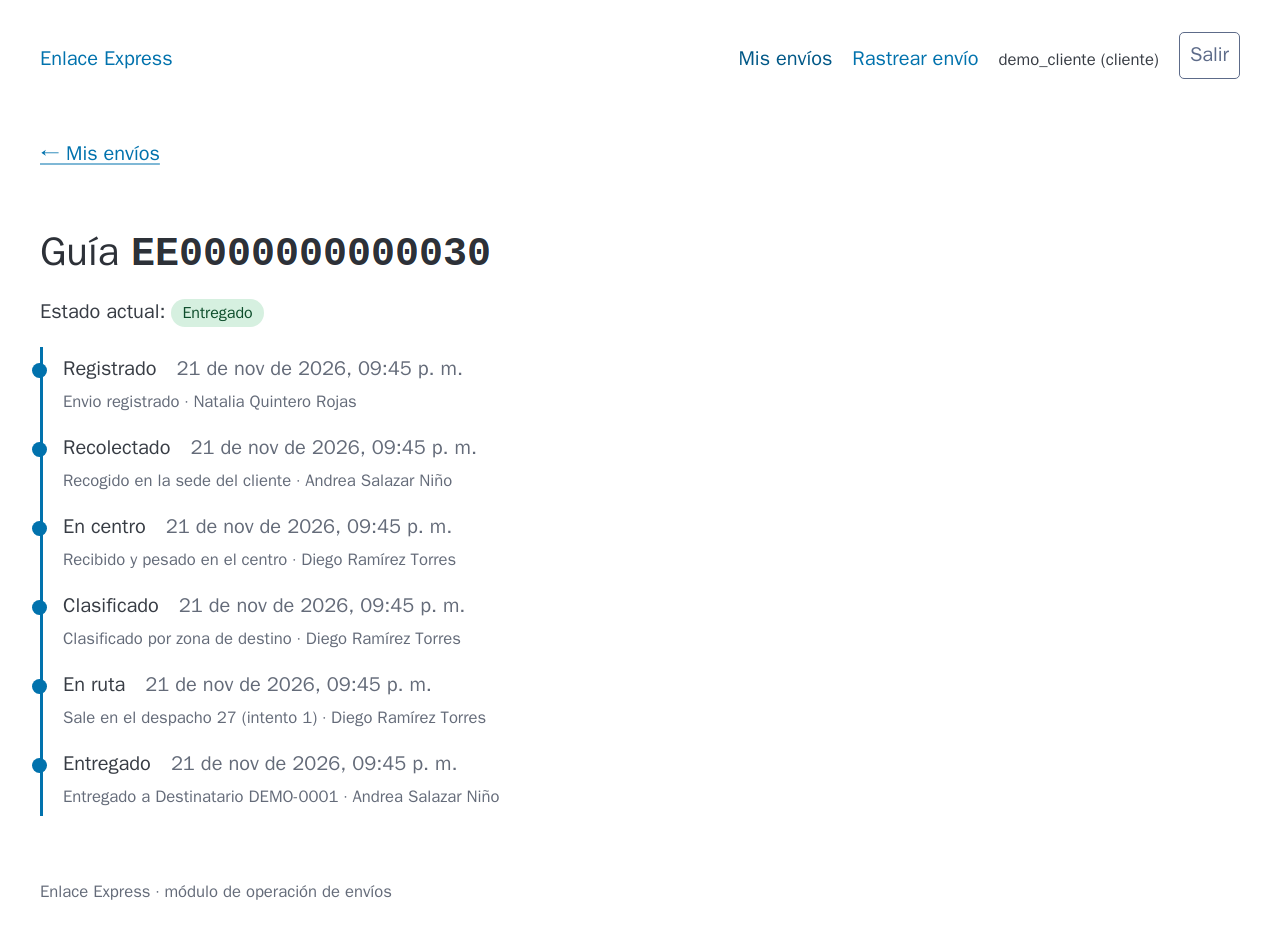
\includegraphics[width=0.75\linewidth]{figures/15_cliente_recorrido.png}
\caption{Recorrido de un envío entregado en el portal del cliente.}
\label{fig:proto-cliente}
\end{figure}

\begin{figure}[htbp]
\centering
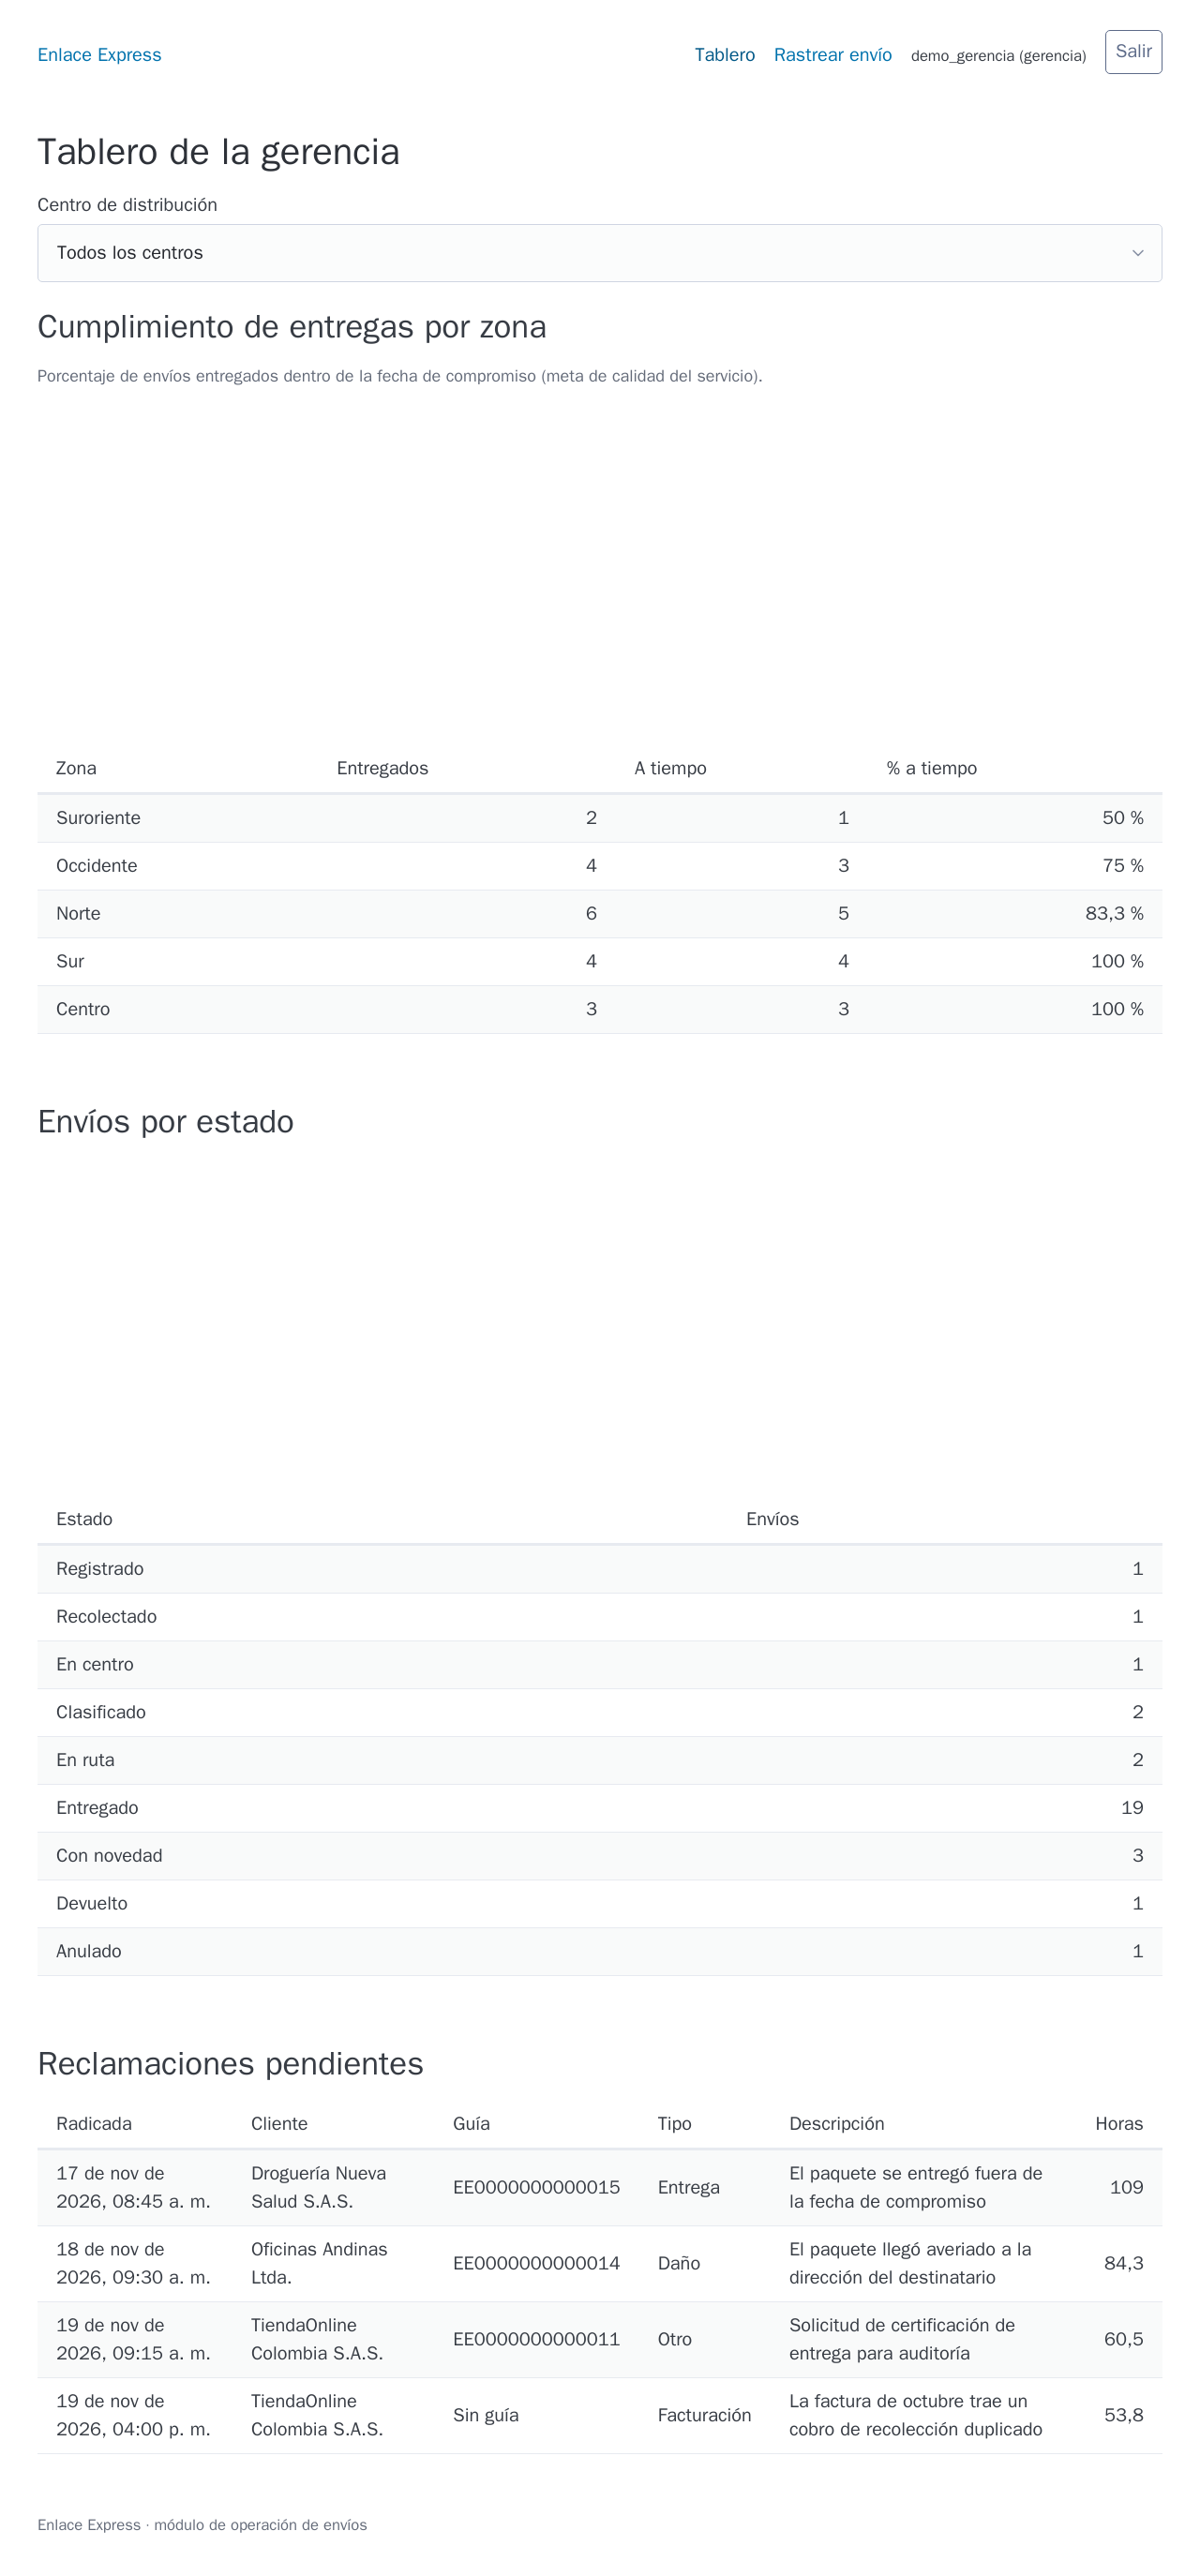
\includegraphics[trim=0 1138 0 0, clip, width=0.65\linewidth]{figures/16_tablero.png}
\caption{Tablero de la gerencia: cumplimiento de entregas por zona y envíos por estado.}
\label{fig:proto-tablero}
\end{figure}

La mesa de servicio también gestiona novedades y reclamaciones. En
\emph{Novedades} ve las novedades abiertas con los teléfonos del destinatario y
del cliente, decide si se reintenta o se devuelve, deja la solución y la
cierra. En \emph{Reclamaciones} radica la reclamación de un cliente, con
una guía opcional que debe ser de un envío de ese cliente (si no lo es, la
aplicación la rechaza), la responde y la cierra. La lista de pendientes marca
con las horas transcurridas las que superan la meta de cuatro horas de la
regla RN14 (figura~\ref{fig:proto-reclamaciones}). El personal del centro, por
su parte, administra los centros y sus zonas en \emph{Centros y zonas}: crea y
modifica, e inactiva un centro en lugar de borrarlo (RN16), y a un centro
inactivo no se le agregan zonas.

\begin{figure}[htbp]
\centering
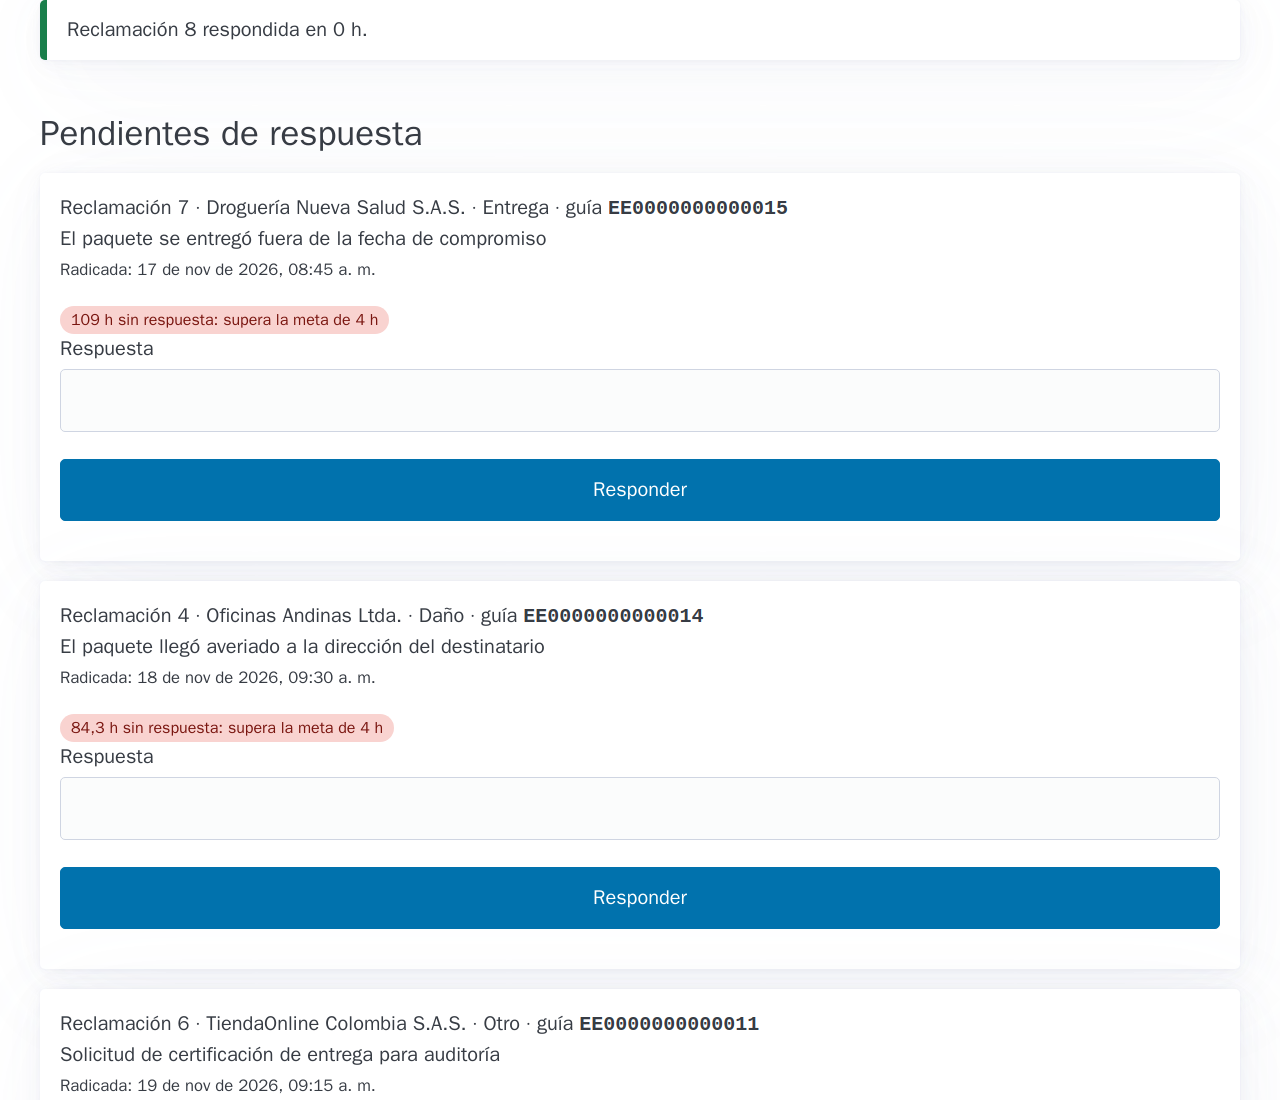
\includegraphics[width=0.7\linewidth]{figures/23_mesa_reclamacion_respondida.png}
\caption{Reclamaciones en la mesa de servicio: aviso de la respuesta registrada y pendientes con las horas transcurridas y la marca de la meta de 4 horas.}
\label{fig:proto-reclamaciones}
\end{figure}

El caso de rechazo sigue con el envío que tuvo novedad: el centro cierra el
despacho, el envío vuelve a la lista de envíos por despachar con un intento
previo y sale en un despacho nuevo; tras una segunda novedad y un tercer
despacho, en el intento 3 la planilla ya no ofrece entregar y solo permite
registrar la devolución (figura~\ref{fig:proto-tercer}), con la que el envío
queda devuelto. La mesa de servicio, por último, intenta anular un envío
ya entregado, y la transición bloqueada se ve en pantalla con el código RN12
(figura~\ref{fig:proto-rn12}).

\begin{figure}[htbp]
\centering
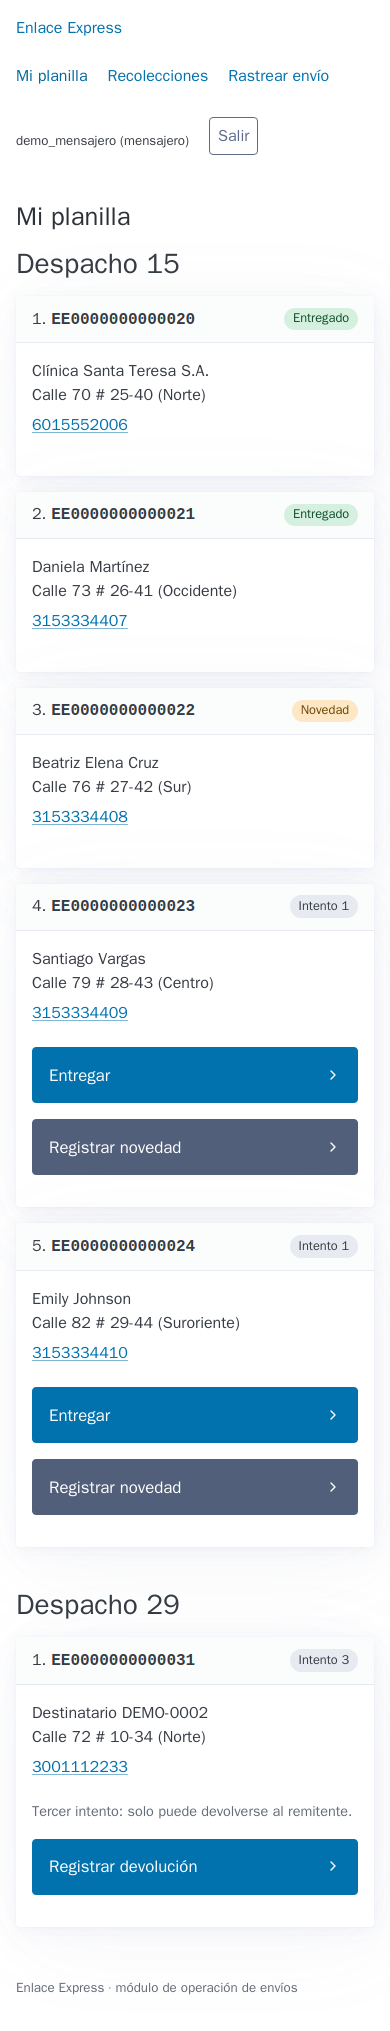
\includegraphics[trim=0 71 0 1560, clip, width=0.42\linewidth]{figures/18_mensajero_tercer_intento_movil.png}
\caption{Tercer intento en la planilla: solo se ofrece registrar la devolución.}
\label{fig:proto-tercer}
\end{figure}

\begin{figure}[htbp]
\centering
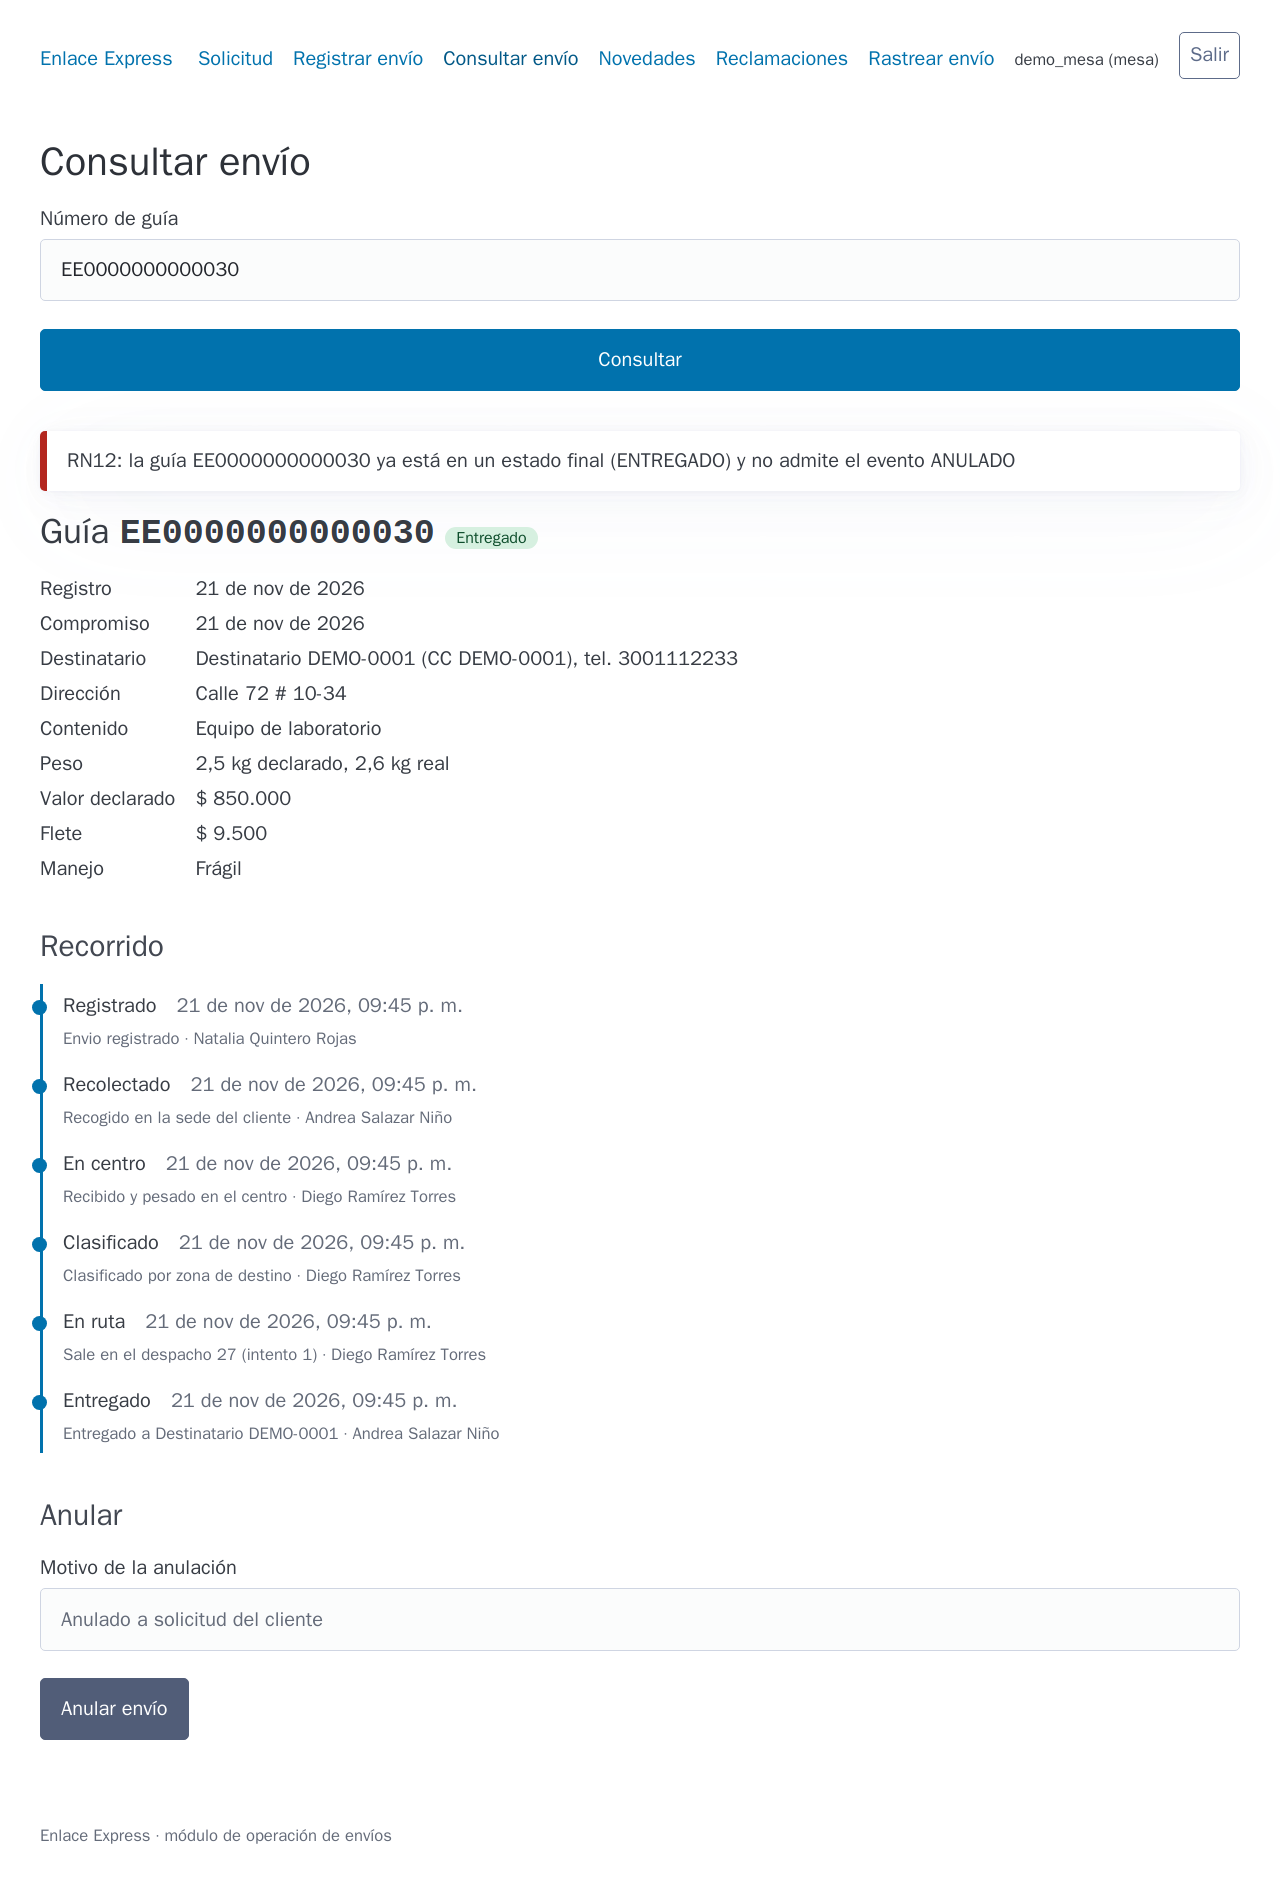
\includegraphics[trim=0 890 0 0, clip, width=0.75\linewidth]{figures/21_rechazo_rn12_anular_entregado.png}
\caption{Rechazo RN12 al intentar anular un envío ya entregado.}
\label{fig:proto-rn12}
\end{figure}

\textbf{Pruebas de la aplicación.} Hay tres niveles:

\begin{itemize}[itemsep=2pt]
  \item \textbf{Unitarias.} Las pruebas del dominio y de la infraestructura no
        usan la base de datos: 60 pruebas en 10 clases, que cubren las reglas
        del dominio (RN02, RN03, RN05, RN07, RN10, RN11, RN12, RN14 y RN15), el
        ciclo de vida del envío, la gestión de novedades y reclamaciones, los
        centros y las zonas, y la traducción de errores de Oracle.
  \item \textbf{De integración.} 39 pruebas en 8 clases que usan Oracle: los
        mapeadores y la unidad de trabajo contra la base (15) y la API por
        HTTP real con sesión y token CSRF (24), incluidos el flujo principal, los
        rechazos y la devolución en el tercer intento, los permisos por rol, el
        identificador de cliente, el rastreo público sin datos personales y el
        límite de consultas.
        Por defecto usan el Oracle del compose. Con la variable de entorno
        \texttt{ENLACE\_TESTCONTAINERS=true}, o con el perfil de Maven
        \texttt{testcontainers}, levantan en cambio un solo contenedor de
        Oracle, con la misma imagen, para toda la corrida: instalan el
        esquema con \texttt{database/install.sh}, generan sus contraseñas al azar y no
        dependen del compose ni del \texttt{.env}. Es el modo de la
        integración continua (subsección~\ref{sec:proto-despliegue}).
  \item \textbf{De punta a punta.} Un recorrido en un navegador sin
        cabeza (Chromium con Playwright) de 27 pasos con los usuarios de
        demostración, que da 27 OK y 0 fallas y guarda 25 capturas, de las
        que esta subsección usa once.
\end{itemize}

La tabla~\ref{tab:proto-pruebas} da el resultado de
\texttt{mvn verify} por clase: 99 pruebas, ninguna con falla. La
demostración se reconstruye con un solo comando,
\texttt{demo/start.sh}, que reinstala la base, compila la
aplicación, la levanta y crea un usuario de demostración por rol (gerencia,
centro, mesa, mensajero y cliente); la contraseña de esos usuarios sale de
una variable de entorno y no está en el repositorio ni en este documento.

% Fuente: docs/evidence/12_pruebas_backend.txt y docs/evidence/10_aplicacion/resumen.txt
{\singlespacing\small
\begin{longtable}{L{4.8cm} L{6.8cm} >{\raggedleft\arraybackslash}p{1.7cm}}
\caption{Pruebas automáticas de la aplicación, por clase.}
\label{tab:proto-pruebas}\\
\toprule
\textbf{Clase} & \textbf{Qué prueba} & \textbf{Pruebas} \\
\midrule
\endfirsthead
\toprule
\textbf{Clase} & \textbf{Qué prueba} & \textbf{Pruebas} \\
\midrule
\endhead
\bottomrule
\endfoot
ConversorTiposTest & Conversión de tipos entre Java y Oracle & 3 \\
TraductorErroresOracleTest & Conversión de errores de Oracle en excepciones del dominio & 11 \\
AsignacionDespachoTest & Intentos de entrega y sus resultados (RN05, RN07, RN08) & 8 \\
DespachoTest & Armado y cierre del despacho (RN10, RN11) & 6 \\
EnvioTest & Registro, clasificación, anulación y eventos del envío (RN02, RN03, RN05, RN12) & 8 \\
CicloDeVidaEnvioTest & Transiciones de estado (RN12) & 6 \\
SolicitudRecoleccionTest & Solicitud de recolección (RN15) & 4 \\
ReclamacionTest & Reclamaciones: radicar, responder (RN14), cerrar y la meta de 4 horas & 6 \\
NovedadTest & Gestión y cierre de la novedad & 3 \\
CentroZonaTest & Centros y zonas: validación, estado y zonas de centros inactivos & 5 \\
\midrule
\multicolumn{2}{l}{\textbf{Unitarias}} & \textbf{60} \\
\midrule
CatalogoEstadosIT & Los catálogos del dominio coinciden con los de la base & 2 \\
FlujoPrincipalIT & El flujo principal con los mapeadores contra Oracle & 2 \\
InfraestructuraJdbcIT & Cuentas de servicio, unidad de trabajo, identificador de cliente y traducción de errores & 11 \\
FlujoApiIT & Flujo principal por la API, rechazos y devolución en el tercer intento & 3 \\
GestionMesaCentroIT & Novedades, reclamaciones y centros y zonas por la API, con sus rechazos & 5 \\
OpenApiIT & La documentación OpenAPI y Swagger UI se entregan sin sesión y las rutas de los roles siguen protegidas & 3 \\
SaludIT & Chequeo de salud de la aplicación y la base & 1 \\
SeguridadIT & Registro, sesión, CSRF, roles, rastreo público y límite por dirección IP & 12 \\
\midrule
\multicolumn{2}{l}{\textbf{De integración}} & \textbf{39} \\
\midrule
\multicolumn{2}{l}{\textbf{Total}} & \textbf{99} \\
\end{longtable}
\par}


%-----------------------------------------------------------------------
\subsubsection{Extensiones fuera del módulo}
\label{sec:proto-extensiones}

El prototipo es el módulo de operación de envíos funcionando. Se permite
extenderlo fuera del módulo solo para probar un caso de uso completo o para
hacer una prueba real del sistema. Cada extensión se registra en
\texttt{docs/extensions.md} con lo que agrega, el caso de uso que permite
probar y por qué no está en el módulo; sus scripts van en una carpeta aparte,
\texttt{database/extensions}, y no modifican las 19 tablas del módulo. Se
hicieron dos extensiones, E1 y E2.

\textbf{E1. Usuarios de la aplicación y códigos de activación.} El módulo no
tiene credenciales: las cuentas de usuario y la autenticación no hacen
parte de la operación de envíos, y en una empresa real vendrían del
directorio de usuarios. Pero sin cuentas no se puede probar ningún caso
de uso que exija iniciar sesión (los de U1 a U4 y el seguimiento de U9 con
cuenta) ni la alta de cuentas del caso de uso de gestión de usuarios y
roles. Por eso se agregó E1, con los objetos de la
tabla~\ref{tab:proto-e1}.

{\singlespacing\small
\begin{longtable}{L{3.6cm} L{2.2cm} L{8.2cm}}
\caption{Objetos de la extensión E1.}
\label{tab:proto-e1}\\
\toprule
\textbf{Objeto} & \textbf{Tipo} & \textbf{Qué es} \\
\midrule
\endfirsthead
\toprule
\textbf{Objeto} & \textbf{Tipo} & \textbf{Qué es} \\
\midrule
\endhead
\bottomrule
\endfoot
USUARIO\_\allowbreak APLICACION & Tabla & Cuenta de acceso: nombre de usuario único, hash BCrypt de la contraseña, rol de la aplicación (GERENCIA, CENTRO, MESA, MENSAJERO o CLIENTE), vínculo con un empleado (una cuenta por empleado) o con un cliente (varias cuentas por empresa), estado y fechas de creación y de último ingreso. \\
CODIGO\_\allowbreak ACTIVACION & Tabla & Código de un solo uso y con vencimiento, emitido para un empleado o para un cliente. Solo se guarda su hash SHA-256; registra cuándo se usó y qué cuenta lo usó. \\
Cuatro índices & Índices & Sobre las claves foráneas, en TS\_ENLACE\_INDICES como los demás. \\
pkg\_codigos\_\allowbreak activacion & Paquete & Solo para el administrador de la base de datos: genera el código de un empleado activo (por documento) o de un cliente activo (por NIT), con vigencia de 72 horas por defecto. \\
pkg\_seguridad & Paquete & Lo usa la aplicación: registro de empleados y clientes con su código, datos para el inicio de sesión y registro del último ingreso. \\
\end{longtable}
\par}

Las dos tablas no se conceden a ningún rol: la única puerta es el paquete
\texttt{pkg\_seguridad}, con permiso de ejecución para el rol cliente. La
parte pública de la aplicación (inicio de sesión, registro y rastreo por
guía) trabaja antes de saber quién es el usuario, y usa la cuenta de
servicio de menor privilegio, \texttt{svc\_cliente}.

\textbf{Cómo se registra un usuario.} El administrador genera un código para
el empleado (con su documento) o para la empresa cliente (con su NIT) y se
lo entrega. La persona abre la aplicación y escribe su documento o el NIT
de su empresa, el código, un nombre de usuario y una contraseña. La
aplicación calcula el hash de la contraseña y llama a \texttt{pkg\_seguridad};
la base de datos nunca ve la contraseña, y del código solo guarda el hash, no el
código en claro, que se muestra una vez al generarlo. El código se usa una
sola vez.

\textbf{Reglas que aplica E1.}

\begin{itemize}[itemsep=2pt]
  \item El código es de un solo uso y vence. Se bloquea con
        \texttt{SELECT \ldots{} FOR UPDATE} al usarlo, para que dos
        registros simultáneos no lo usen dos veces.
  \item El empleado debe existir y estar ACTIVO, y el cliente debe estar
        ACTIVO.
  \item El rol se deriva del cargo y nunca lo elige el usuario: Gerente es
        GERENCIA, Auxiliar de centro es CENTRO, Agente de mesa de servicio
        es MESA y Mensajero, si tiene fila en MENSAJERO, es MENSAJERO. Otro
        cargo no tiene acceso.
  \item Un documento inexistente, un código ajeno, usado o vencido dan el
        mismo mensaje, para no revelar cuál dato falló.
  \item Una cuenta cuyo empleado se retira o cuyo cliente se inactiva queda
        INACTIVA de inmediato en el inicio de sesión.
  \item Los errores van en el rango ORA-20101 a ORA-20112, con mensajes que
        empiezan por \texttt{E1:}, fuera del rango de las reglas RN del
        módulo.
\end{itemize}

\textbf{Pruebas de E1.} El script
\texttt{database/tests/test-e1.sh} ejecuta 74 casos, todos con el
resultado previsto (tabla~\ref{tab:proto-pruebas-e1}). Incluyen, entre otros,
la reutilización de un código (ORA-20101), un código vencido o de otro
empleado, un empleado retirado, un nombre de usuario repetido (ORA-20102),
un cargo sin acceso (ORA-20103), una segunda cuenta para el mismo empleado
(ORA-20105) y que las otras cuatro cuentas de servicio no puedan leer ni
ejecutar nada de E1.

% Fuente: docs/evidence/09_extension_e1.txt
{\singlespacing\small
\begin{longtable}{L{9.0cm} >{\raggedleft\arraybackslash}p{1.6cm} >{\raggedleft\arraybackslash}p{1.8cm}}
\caption{Casos de prueba de la extensión E1.}
\label{tab:proto-pruebas-e1}\\
\toprule
\textbf{Parte} & \textbf{Casos} & \textbf{Fallas} \\
\midrule
\endfirsthead
\toprule
\textbf{Parte} & \textbf{Casos} & \textbf{Fallas} \\
\midrule
\endhead
\bottomrule
\endfoot
Lógica de los paquetes y restricciones de las tablas (propietario) & 48 & 0 \\
La aplicación con \texttt{svc\_cliente}: registro, inicio de sesión y permisos & 10 & 0 \\
Las otras cuatro cuentas de servicio no tienen acceso a E1 & 16 & 0 \\
\midrule
\textbf{Total} & \textbf{74} & \textbf{0} \\
\end{longtable}
\par}

{\sloppy
\textbf{E2. Vista de rastreo público.} El documento define el seguimiento
con la vista \texttt{v\_\allowbreak seguimiento\_\allowbreak envio}, para la mesa de servicio y
para el cliente con cuenta. Esa vista trae la observación y el responsable
de cada evento, que pueden contener nombres (por ejemplo, ``Entregado a
Recepción del edificio''), y no trae la zona. El rastreo público, que la
decisión de diseño pide sin cuenta y sin datos personales, necesita
la zona de destino, y la cuenta \texttt{svc\_\allowbreak cliente} no puede leer las tablas
ENVIO ni ZONA. En lugar de cambiar una de las siete vistas del módulo o
de ampliar los permisos del rol cliente, se agregó la vista
\texttt{v\_\allowbreak rastreo\_\allowbreak publico}: número de guía, identificador del evento
(solo para ordenar), fecha y hora, estado y zona de cada evento. Es de solo
lectura y se concede únicamente al rol cliente. No incluye la observación, el
responsable ni ningún dato del destinatario o del cliente.
\par}

Con E2 se prueba el seguimiento público de un envío sin cuenta: cualquier
persona con el número de guía ve estados, fechas y zona, sin nombres,
direcciones ni teléfonos. Como las guías son consecutivas y se podrían recorrer,
la aplicación limita además las consultas por dirección IP (30 por minuto por
defecto).

% Fuente: docs/evidence/03_prueba_permisos.txt (svc_cliente) y 01_verificacion_cifras.txt
Las pruebas de permisos de la subsección~\ref{sec:proto-bd} cubren E2: con
la cuenta \texttt{svc\_cliente}, la consulta de \texttt{v\_rastreo\_publico}
pasa, y leer las tablas ENVIO y ZONA se rechaza (ORA-00942). La
aplicación muestra el resultado en la captura del rastreo público de la
subsección~\ref{sec:proto-aplicacion}.

\textbf{Las cifras del módulo no cambian.} La verificación de cifras de
la tabla~\ref{tab:proto-cifras} cuenta los objetos del módulo por una lista
explícita, y con las extensiones instaladas sigue dando 19 tablas, 59
índices, 7 vistas, 6 disparadores y 1 procedimiento. Las extensiones
tienen sus propias filas, aparte: E1 agrega 2 tablas y ningún privilegio
concedido a los roles, y E2 agrega 1 vista; las tres dan OK
(tabla~\ref{tab:proto-cifras-ext}).

% Fuente: docs/evidence/01_verificacion_cifras.txt
{\singlespacing\small
\begin{longtable}{L{8.2cm} >{\raggedleft\arraybackslash}p{1.9cm} >{\raggedleft\arraybackslash}p{1.9cm} L{2.0cm}}
\caption{Cifras de las extensiones, aparte de las del módulo.}
\label{tab:proto-cifras-ext}\\
\toprule
\textbf{Cifra} & \textbf{Esperado} & \textbf{Obtenido} & \textbf{Resultado} \\
\midrule
\endfirsthead
\toprule
\textbf{Cifra} & \textbf{Esperado} & \textbf{Obtenido} & \textbf{Resultado} \\
\midrule
\endhead
\bottomrule
\endfoot
Extensión E1: tablas & 2 & 2 & OK \\
Extensión E1: privilegios concedidos a roles & 0 & 0 & OK \\
Extensión E2: vistas & 1 & 1 & OK \\
\end{longtable}
\par}


%-----------------------------------------------------------------------
\subsubsection{Concurrencia}
\label{sec:proto-concurrencia}

\textbf{El problema.} En la operación, dos usuarios pueden actuar al
mismo tiempo sobre el mismo envío o el mismo despacho. Por ejemplo, la mesa
de servicio anula un envío en el momento en que el centro lo incluye en un
despacho; o dos centros arman despachos que comparten un envío. Si cada
transacción lee el estado, decide y escribe sin coordinarse, las dos
pueden decidir con el mismo estado de partida y dejar el envío con eventos
que no siguen el ciclo de vida de la tabla~\ref{tab:transiciones}
(por ejemplo, EN\_RUTA después de ANULADO).

\textbf{La solución: bloqueo pesimista.} Toda transacción que cambia el
estado de un envío o de un despacho bloquea primero esa fila con
\texttt{SELECT \ldots{} FOR UPDATE}. Mientras una transacción tiene la
fila bloqueada, otra que quiera cambiarla espera; cuando la primera
confirma o deshace, la segunda sigue y, al leer, ve el estado que dejó la
primera. Así las reglas del dominio y los disparadores trabajan siempre
sobre el estado actual y la segunda transacción se rechaza, con el mensaje
de la regla correspondiente, si ya no es válida.

Se eligió el bloqueo pesimista en lugar del optimista por tres razones.
Las transacciones son cortas (cada operación toma una conexión al
empezar y la devuelve al terminar), de modo que el bloqueo dura milisegundos y nadie
espera mientras un usuario llena un formulario. Un conflicto sobre un mismo
envío es poco frecuente, pero sus consecuencias son costosas: eventos
fuera de orden o un envío entregado dos veces. Y el control optimista
exigiría una columna de versión en las tablas y repetir la operación
cuando alguien se anticipó, algo que el modelo no tiene y que complica la
aplicación sin beneficio para este volumen.

\textbf{Cómo lo aplican las transacciones y la aplicación.} Las
transacciones de la subsección~\ref{sec:proto-transacciones} empiezan con el
bloqueo de la fila que cambia. La aplicación hace lo mismo: cada caso de
uso abre una unidad de trabajo, que toma una conexión de la cuenta de
servicio del rol, sin confirmación automática; la transacción la maneja
la propia aplicación y no un marco externo. Cada operación bloquea,
antes de leer el estado y decidir, lo que muestra la
tabla~\ref{tab:proto-bloqueos}.

{\singlespacing\small
\begin{longtable}{L{5.0cm} L{9.0cm}}
\caption{Filas que bloquea cada operación de la aplicación.}
\label{tab:proto-bloqueos}\\
\toprule
\textbf{Operación} & \textbf{Filas bloqueadas, en orden} \\
\midrule
\endfirsthead
\toprule
\textbf{Operación} & \textbf{Filas bloqueadas, en orden} \\
\midrule
\endhead
\bottomrule
\endfoot
Registrar envío & La solicitud de recolección. \\
Anular un envío & El envío. \\
Recolectar & La solicitud y, uno por uno, sus envíos. \\
Recibir y clasificar & El envío. \\
Armar el despacho de entrega & Cada envío del despacho, en orden de número de guía. \\
Registrar entrega, novedad o devolución & El envío y la asignación. \\
Cerrar el despacho & El despacho. \\
\end{longtable}
\par}

\textbf{Orden de bloqueo.} Cuando una operación bloquea varias filas, dos
operaciones simultáneas podrían quedar esperándose una a la otra
(interbloqueo). Para evitarlo, al armar un despacho la aplicación elimina
las guías repetidas y las ordena por número de guía antes de bloquearlas, de
modo que dos despachos que compartan envíos los bloquean en el mismo
orden y uno simplemente espera al otro.

\textbf{Instantes distintos (C5).} El índice único sobre el número de guía
y la fecha y hora del evento impide que un envío tenga dos eventos en el
mismo instante. Cuando una transacción inserta varios eventos del mismo
envío, la aplicación asigna a cada uno un instante distinto, siempre
posterior al último evento de la guía; el tipo de dato guarda
microsegundos. Las transacciones de prueba hacen lo mismo con una función
que calcula ese instante:

\begin{lstlisting}[style=sqlpro]
FUNCTION instante(p_guia IN VARCHAR2) RETURN TIMESTAMP IS
    v_i TIMESTAMP;
BEGIN
    SELECT GREATEST(LOCALTIMESTAMP,
                    NVL(MAX(fecha_hora), LOCALTIMESTAMP) + INTERVAL '1' SECOND)
    INTO   v_i FROM evento_envio WHERE numero_guia = p_guia;
    RETURN v_i;
END instante;
\end{lstlisting}

\textbf{La prueba.} El script \texttt{database/transactions/concurrency.sh}
reproduce el conflicto con dos sesiones de verdad sobre el envío
EE0000000000028. La sesión A, con la cuenta del centro
(\texttt{svc\_centro}), bloquea la fila con \texttt{SELECT \ldots{} FOR UPDATE}
y no confirma. La sesión B, con la cuenta de la mesa (\texttt{svc\_mesa}),
intenta lo mismo con la opción \texttt{NOWAIT}, que en lugar de esperar
devuelve el error ORA-00054 (recurso ocupado), y reintenta cada segundo.
Se usa \texttt{NOWAIT} solo para que el conflicto quede a la vista sin dejar
una sesión colgada; la aplicación, en cambio, espera el bloqueo. Si Oracle
devuelve ORA-00054 a la aplicación, esta lo traduce a una respuesta de
conflicto. La tabla~\ref{tab:proto-concurrencia} muestra la línea de
tiempo: B recibe ORA-00054 en los seis intentos que hace mientras A tiene
la fila; cuando A deshace, B consigue el bloqueo en el intento 7.

% Fuente: docs/evidence/06_transacciones/concurrencia.txt
{\singlespacing\small
\begin{longtable}{L{2.4cm} L{1.4cm} L{9.6cm}}
\caption{Línea de tiempo de la prueba de concurrencia.}
\label{tab:proto-concurrencia}\\
\toprule
\textbf{Hora} & \textbf{Sesión} & \textbf{Hecho} \\
\midrule
\endfirsthead
\toprule
\textbf{Hora} & \textbf{Sesión} & \textbf{Hecho} \\
\midrule
\endhead
\bottomrule
\endfoot
16:59:34.534 & A & Obtiene el bloqueo sobre EE0000000000028, sin COMMIT. \\
16:59:35.037 & B & Intento 1 rechazado: ORA-00054, la fila está bloqueada por A. \\
16:59:36.038 & B & Intento 2 rechazado: ORA-00054. \\
16:59:37.038 & B & Intento 3 rechazado: ORA-00054. \\
16:59:38.039 & B & Intento 4 rechazado: ORA-00054. \\
16:59:39.039 & B & Intento 5 rechazado: ORA-00054. \\
16:59:40.040 & B & Intento 6 rechazado: ORA-00054. \\
16:59:40.537 & A & ROLLBACK, bloqueo liberado. \\
16:59:41.040 & B & Intento 7 consigue el bloqueo sobre EE0000000000028. \\
16:59:41.041 & B & ROLLBACK (la prueba no modifica datos). \\
\end{longtable}
\par}

\textbf{Las restricciones siguen siendo la garantía final.} El bloqueo
evita que dos transacciones decidan con el mismo estado, pero no es la
única defensa. Si dos transacciones llegaran a escribir a la vez lo mismo,
la base de datos las rechaza por sus restricciones: una segunda prueba de
entrega o una segunda novedad para el mismo intento viola una restricción
UNIQUE (ORA-00001, casos de T6 y T7), y dos eventos de una guía en el mismo
instante violan el índice único de guía y fecha y hora. Los disparadores
validan el ciclo de vida en la base aunque la aplicación se saltara el
dominio. Por eso las reglas de negocio no dependen de que todas las
aplicaciones bloqueen bien.


%-----------------------------------------------------------------------
\subsubsection{Despliegue y CI/CD}
\label{sec:proto-despliegue}
% Actualizar cuando se cree la máquina virtual y el dominio o se active el CD (los artefactos ya existen y se probaron en el equipo)

\textbf{Estado actual.} Hoy el prototipo corre en el equipo de desarrollo:
Oracle Database 23c Free en un contenedor Docker, definido en el archivo
\texttt{docker-compose.yml}, y la aplicación como un programa Java. Los
artefactos para publicarlo en un servidor existen y se probaron en el equipo
(más abajo), pero todavía no hay una máquina virtual ni un dominio. Todo se
reconstruye desde cero con tres comandos:

\begin{enumerate}[itemsep=2pt]
  \item \texttt{docker compose up -d} levanta la base de datos y espera a que
        esté lista.
  \item \texttt{database/install.sh} reinstala el esquema, los datos y las
        extensiones, y verifica las cifras del documento. Como alternativa,
        \texttt{demo/start.sh} hace además la aplicación: la
        compila, la levanta y crea los usuarios de demostración.
  \item \texttt{database/generate-evidence.sh} repite las pruebas, las consultas, las
        transacciones y los informes y regenera todas las evidencias de
        \texttt{docs/evidence/}.
\end{enumerate}

Las contraseñas no están en el repositorio: salen de un archivo \texttt{.env}
que no se versiona, del que solo se guarda una plantilla. El
contenedor usa la zona horaria America/Bogota, igual que la aplicación.

\textbf{Integración continua.} {\sloppy El flujo de GitHub Actions es el archivo
\texttt{ci.yml} de la carpeta \texttt{.github/workflows}. Se ejecuta en cada cambio a la rama
principal y en cada solicitud de integración, en una máquina Ubuntu del
servicio, y tiene dos trabajos que corren en paralelo:\par}

\begin{itemize}[itemsep=2pt]
  \item \textbf{Compilar y probar.} Prepara Java 21 y Node 22, compila el
        frontend, y compila el backend y corre sus 99 pruebas con
        \texttt{mvn verify}. Las pruebas de integración usan Testcontainers:
        levantan un solo contenedor de Oracle con la misma imagen que usa el
        compose, instalan el esquema con \texttt{database/install.sh}, que verifica
        las cifras del documento en modo estricto, y apuntan la aplicación y las
        pruebas a ese contenedor. Si algo falla, guarda los informes de las
        pruebas.
  \item \textbf{Cifras del documento.} Instala el esquema en un Oracle
        desechable y falla si alguna de las cifras del documento (19 tablas, 59
        índices, 6 disparadores, etc.) no coincide.
\end{itemize}

El flujo no usa secretos: las contraseñas de Oracle se generan al azar en cada
corrida y viajan por variables de entorno. Las mismas pruebas pueden correrse
en el equipo, contra el Oracle del compose (modo normal) o con
Testcontainers, que no depende de él. Como el repositorio no tiene un
servidor remoto, el flujo no se ha ejecutado en GitHub: se validó su sintaxis
y se ejecutaron sus mismos pasos en el equipo con \texttt{ci/local.sh}, que
compila el frontend, corre \texttt{mvn verify} con Testcontainers y verifica las
cifras, de principio a fin, sin fallas y en unos dos minutos
(\texttt{docs/evidence/12\_pruebas\_backend.txt}).

\textbf{Artefactos de despliegue.} La carpeta \texttt{deploy/} reúne lo
necesario para publicar el prototipo según el diseño definido, y se probó en el
equipo:

\begin{itemize}[itemsep=2pt]
  \item \textbf{Imagen de la aplicación.} El \texttt{Dockerfile} es multietapa:
        compila el frontend (Node 22) y el backend (Maven con JDK 21) y deja un
        JRE 21 con versión fija, un usuario sin privilegios, la zona horaria
        America/Bogota y una comprobación de salud contra \texttt{/api/salud}.
        Las imágenes base son para x86 y ARM. Aquí se construyó para x86; la de
        ARM no se construyó porque el equipo no tiene el emulador QEMU, y la
        construirá el flujo de entrega continua.
  \item \textbf{Compose de producción.} Levanta Oracle 23c Free con un volumen
        con nombre y sin publicar su puerto, la aplicación y Caddy (con versión
        fija) como proxy inverso. Las contraseñas y el dominio salen de un
        archivo \texttt{.env}.
  \item \textbf{HTTPS.} Caddy obtiene y renueva el certificado del dominio
        configurado; con el dominio \texttt{localhost} usa su certificado
        interno, lo que permitió probarlo en el equipo. La aplicación va detrás
        del proxy con las cookies marcadas como seguras y con el límite de
        consultas del rastreo público calculado por la dirección IP que agrega
        el proxy.
  \item \textbf{Esquema.} Un script instala el esquema una sola vez y no hace
        nada si ya existe; un cambio de esquema se hace reinstalando con él.
  \item \textbf{Entrega continua.} El flujo de GitHub Actions \texttt{cd.yml}
        se ejecuta cuando la integración continua de la rama principal termina
        bien: construye la imagen para x86 y ARM, la publica en el registro de
        contenedores de GitHub y, si hay un servidor configurado con sus
        secretos, actualiza por SSH solo los contenedores de la aplicación. Como
        el repositorio no tiene un servidor remoto, el flujo no se ha ejecutado;
        solo se validó su sintaxis.
  \item \textbf{Respaldo.} Si no se consigue la máquina virtual, se presenta
        desde el equipo propio con Docker y un túnel de Cloudflare, que da
        HTTPS gratuito pero no tiene entrega continua; el procedimiento está
        explicado en \texttt{deploy/README.md}.
\end{itemize}

\textbf{Prueba en el equipo.} El script \texttt{deploy/test-local.sh}
construye la imagen, levanta el compose de producción con el dominio
\texttt{localhost}, instala el esquema, hace las comprobaciones de la
tabla~\ref{tab:proto-despliegue} con \texttt{curl} a través de Caddy y, al terminar,
baja el compose y borra sus volúmenes. Dio 21 de 21 comprobaciones correctas.
Entre ellas, que el límite de consultas cuenta la dirección IP real de cada
cliente y no la del proxy: desde el equipo, las primeras 30 consultas dan 200 y la
31 da 429, un encabezado \texttt{X-Forwarded-For} falso no evita el límite, y
otro cliente con otra dirección, desde otro contenedor, sigue consultando.

% Fuente: docs/evidence/14_despliegue_local.txt
{\singlespacing\small
\begin{longtable}{L{4.0cm} L{9.2cm}}
\caption{Comprobaciones de la prueba local del despliegue.}
\label{tab:proto-despliegue}\\
\toprule
\textbf{Aspecto} & \textbf{Comprobación (todas dieron OK)} \\
\midrule
\endfirsthead
\toprule
\textbf{Aspecto} & \textbf{Comprobación (todas dieron OK)} \\
\midrule
\endhead
\bottomrule
\endfoot
Imagen & Se construye; la aplicación corre sin privilegios, con la zona horaria America/Bogota. \\
Oracle & Está sano y no publica ningún puerto; la aplicación solo se alcanza por Caddy. \\
Esquema & Se instala con las cifras del documento en modo estricto y una segunda ejecución no lo reinstala. \\
HTTPS & \texttt{/api/salud} responde 200 por HTTPS, HTTP redirige a HTTPS, Caddy agrega Strict-Transport-Security y se sirve la aplicación web. \\
Rastreo público & La guía EE0000000000003 muestra su estado ENTREGADO sin sesión. \\
Rutas protegidas & \texttt{/api/mesa/clientes} da 401 sin sesión y 200 con la sesión de la mesa, creada con un código de activación. \\
Cookies & Las cookies \texttt{XSRF-TOKEN} y \texttt{JSESSIONID} salen con Secure, y la de sesión con HttpOnly. \\
Límite por IP & 30 consultas dan 200 y la 31 da 429; un \texttt{X-Forwarded-For} falso no evita el límite; otro cliente con otra IP no queda limitado. \\
\end{longtable}
\par}

\textbf{Lo que falta.} Quedan por hacer, y requieren las cuentas del autor,
crear la máquina virtual gratuita de Oracle Cloud (Ampere A1), el subdominio
de DuckDNS y los secretos del repositorio que usa la entrega continua. Los pasos
están en \texttt{deploy/README.md}.

Se descartaron otras opciones: Vercel, porque no aloja Oracle y su modelo de
funciones no encaja con una sesión guardada en el servidor; Render con el plan
gratuito, porque tiene 512 MB de memoria, se apaga tras 15 minutos sin
tráfico y no tiene Oracle; y Autonomous Database gratuita, porque no permite
crear espacios de tablas, lo que contradice el diseño físico del
capítulo~5.

